%\documentclass{article}
%
%\usepackage{fancyhdr}
%\usepackage{extramarks}
%\usepackage{amsmath}
%\usepackage{amsthm}
%\usepackage{amsfonts}
%\usepackage{tikz}
%\usepackage{enumerate}
%\usepackage{graphicx}
%\graphicspath{ {images/} }
%\usepackage[plain]{algorithm}
%\usepackage{algpseudocode}
%\usepackage[document]{ragged2e}
%\usepackage{textcomp}
%\usepackage{color}   %May be necessary if you want to color links
%\usepackage{import}
%\usepackage{hyperref}
%\hypersetup{
%    colorlinks=true, %set true if you want colored links
%    linktoc=all,     %set to all if you want both sections and subsections linked
%    linkcolor=black,  %choose some color if you want links to stand out
%}
%
%\usetikzlibrary{automata,positioning}
%
%
%% Basic Document Settings
%
%
%\topmargin=-0.45in
%\evensidemargin=0in
%\oddsidemargin=0in
%\textwidth=6.5in
%\textheight=9.0in
%\headsep=0.25in
%\setlength{\parskip}{1em}
%
%\linespread{1.1}
%
%\pagestyle{fancy}
%\lhead{\hmwkAuthorName}
%\lfoot{\lastxmark}
%\cfoot{\thepage}
%
%\renewcommand\headrulewidth{0.4pt}
%\renewcommand\footrulewidth{0.4pt}
%
%\setlength\parindent{0pt}
%
%
%\newcommand{\hmwkTitle}{Math Review Notes---Probability}
%\newcommand{\hmwkAuthorName}{\textbf{G. Faletto} }
%
%
%%%%%% Title Page
%
%
%\title{
%    \vspace{2in}
%    \textmd{\textbf{ \hmwkTitle}}\\
%}
%
%\author{Gregory Faletto}
%\date{}
%
%\renewcommand{\part}[1]{\textbf{\large Part \Alph{partCounter}}\stepcounter{partCounter}\\}
%
%
%%%%%% Various Helper Commands
%
%
%%%%%% Useful for algorithms
%\newcommand{\alg}[1]{\textsc{\bfseries \footnotesize #1}}
%
%%%%%% For derivatives
%\newcommand{\deriv}[2]{\frac{\mathrm{d} #1}{\mathrm{d} #2}}
%
%%%%%% For partial derivatives
%\newcommand{\pderiv}[2]{\frac{\partial #1}{\partial #2}}
%
%%%%%% Integral dx
%\newcommand{\dx}{\mathrm{d}x}
%
%%%%%% Alias for the Solution section header
%\newcommand{\solution}{\textbf{\large Solution}}
%
%%%%%% Probability commands: Expectation, Variance, Covariance, Bias
%\newcommand{\E}{\mathbb{E}}
%\newcommand{\Var}{\mathrm{Var}}
%\newcommand{\Cov}{\mathrm{Cov}}
%\newcommand{\Bias}{\mathrm{Bias}}
%\newcommand\indep{\protect\mathpalette{\protect\independenT}{\perp}}
%\def\independenT#1#2{\mathrel{\rlap{$#1#2$}\mkern2mu{#1#2}}}
%\DeclareMathOperator{\Tr}{Tr}
%
%\theoremstyle{definition}
%\newtheorem{theorem}{Theorem}
%\theoremstyle{definition}
%\newtheorem{proposition}[theorem]{Proposition}
%\theoremstyle{definition}
%\newtheorem{lemma}[theorem]{Lemma}
%\theoremstyle{definition}
%\newtheorem{corollary}{Corollary}[theorem]
%\theoremstyle{definition}
%\newtheorem{definition}{Definition}[section]
%\newtheorem*{remark}{Remark}
%\theoremstyle{definition}
%\newtheorem{exercise}{Exercise}
%\theoremstyle{definition}
%\newtheorem{example}{Example}[section]
%
%%%%%% Tilde
%\newcommand{\textapprox}{\raisebox{0.5ex}{\texttildelow}}
%
%\begin{document}
%
%\maketitle
%
%\pagebreak
%
%\tableofcontents
%
%\
%
%\
%
%\begin{center}
%Last updated \today
%\end{center}
%
%
%
%\newpage
%%
%%%
%%%
%%%
%%%
%%%
%%%
%%%
%%%
%%%%
%%%% Probability

\section{Probability}

These are my notes from taking Math 505A at USC taught by Sergey Lototsky, Math 541A at USC taught by Steven Heilman, ISE 620 at USC taught by Sheldon Ross (as well as the corresponding textbooks \textit{Introduction to Probability Models} and \textit{Stochastic Processes} by Sheldon Ross) and the textbook \textit{Probability and Random Processes} (Grimmett and Stirzaker) 3rd edition, Statistics 100B at UCLA taught by Nicolas Christou, as well as a few other sources I cite within the text.

\subsection{To Know for Math 505A Midterm 1 (Discrete Random Variables)}

\subsubsection{Definitions}

\begin{definition}The \textbf{probability mass function} of a discrete random variable \(X\) is the function \(f: \mathbb{R} \to [0,1]\) given by \(f(x) = \Pr(X = x)\). \end{definition}

\begin{definition}The \textbf{(cumulative) distribution function} of a discrete random variable \(F\) is given by \[F(x) = \sum_{i:x_i \leq x} f(x_i)\] \end{definition}

\begin{definition}The \textbf{joint probability mass function} \(f: \mathbb{R}^2 \to [0, 1]\) of two discrete random variables \(X\) and \(Y\) is given by

\[
f(x, y) = \Pr(X = x \cap Y = y)
\] \end{definition}

\begin{definition}The \textbf{joint distribution function} \(F: \mathbb{R}^2 \to [0, 1]\) is given by

\[
F(x, y) = \Pr(X \leq x \cap Y \leq y)
\]\end{definition}

\begin{definition}If \(\Pr(B) > 0\) then the \textbf{conditional probability} that \(A\) occurs given that \(B\) occurs is defined to be

\[
\Pr(A \mid B) = \frac{\Pr(A \cap B)}{\Pr(B)}
\]\end{definition}

\begin{definition}\textbf{(Independent sets.)} Let \(A_1, A_2, \ldots\) be subsets of a sample space \(\Omega\), and let \(\mathbb{P}\) be a probability law on \(\Omega\). We say that \(A_1, A_2, \ldots\) are \textbf{independent} if for any finite subset \(S\) of \(\{1, 2, \ldots\}\), we have

\[
\mathbb{P}\bigg( \bigcap_{i \in S} A_i \bigg) = \prod_{i \in S} \mathbb{P}(A_i)
\]

\end{definition}

\begin{definition} \textbf{(Notation.)} Let \(X: \Omega \to \mathbb{R}\) be a random variable. Let \(B \subseteq \mathbb{R}\). We define \(\{X \in B\} := \{\omega \in \Omega: X(\omega) \in B\}\).

\end{definition}

\begin{definition}\textbf{(Independence of random variables.)} Random variables \(X_1, X_2, \ldots\) are \textbf{independent} if for every \(B_1, B_2, \ldots \subseteq \mathbb{R}\), the events \(\{X_1 \in B_1\}, \{X_2 \in B_2\}, \ldots\) are independent; that is, 

\[
\mathbb{P} \bigg( \bigcap_{i=1}^n \{X_i \in B_i\} \bigg) = \prod_{i=1}^n \mathbb{P}(\{X_i \in B_i\})
\]
\end{definition}

\begin{remark}A more informal definition is as follows: Two random variables \(X\) and \(Y\) are \textbf{independent} if and only if \(\Pr(X \cap Y) = \Pr(X) \Pr(Y)\).\end{remark}

\begin{theorem} \textbf{(Law of total probability).} If \(X\) is a random variable and \(Y\) is a discrete random variable taking on values \(y_1, y_2, \ldots, y_n\), then \(\Pr(X) = \sum_i \Pr(X \mid Y = y_i) \cdot \Pr(Y = y_i)\). (Can be used to prove independence.)\end{theorem}

\begin{definition}Two random variables \(X\) and \(Y\) are \textbf{uncorrelated} if \(\E(XY) = \E(X) \E(Y)\).\end{definition} 

\begin{proposition}
\begin{enumerate}[(a)]
\item Two random variables are uncorrelated if and only if their covariance \(\Cov(X, Y) = \E \big[(X - \E(X))(Y - \E(Y))\big] = \E(XY) - \E(X)\E(Y)\)  equals 0. 
\item If \(X\) and \(Y\) are independent then they are uncorrelated.
\end{enumerate}
\end{proposition}

\begin{theorem} If \(X\) and \(Y\) are independent and \(g, h: \mathbb{R} \to \mathbb{R}\), then \(g(X)\) and \(h(Y)\) are also independent. \end{theorem}

\subsubsection{Conditioning}

\begin{definition}The \textbf{conditional distribution function} of \(Y\) given \(X = x\), written \(F_{Y\mid X}( \cdot \mid x)\), is defined by

\[
F_{Y\mid X}( y \mid x) = \Pr(Y \leq y \mid X = x)
\]
\end{definition}

\begin{definition}The \textbf{conditional probability mass function} of \(Y\) given \(X = x\), written \(f_{Y\mid X}( \cdot \mid x)\), is defined by

\[
f_{Y\mid X}( y \mid x) = \Pr(Y = y \mid X = x)
\]
\end{definition}

\begin{theorem}\textbf{Iterated expectations}: 

\begin{enumerate}[(i)]

\item \(\E\big[ \E(X \mid Y) \big] = \E(X)\) \textbf{(Law of Total Expectation)}

\item \(\E \big[ (X \mid Y) \mid Z \big] = \E(X \mid Y)\)

\item \( \E(E(XY \mid Y)) = \E(Y \E(X \mid Y))\)

\end{enumerate}
\end{theorem}

\begin{proof}(i) Discrete case:

\[
\E\big[ \E(X \mid Y) \big] = \sum_{y} \E(X \mid Y = y) \Pr(Y=y) =  \sum_{y} \sum_{x} x \Pr(X=x \mid Y=y) \Pr(Y=y) 
\]

\[
=  \sum_{y} \sum_{x} x \Pr(X=x \cap Y=y) =  \sum_{x}x \sum_{y}  \Pr(X=x \cap Y=y) = \sum_x x \Pr(X=x) = \E(X)
\]

Continuous case:

\[
\E\big[ \E(X \mid Y) \big]  = \int_{-\infty}^\infty \E(X \mid Y = y) f_Y(y) dy = \text{ (by definition 1.75) }  \int_{-\infty}^\infty \bigg( \int_{-\infty}^\infty x f_{X\mid Y}(x \mid y) dx \bigg)  f_Y(y) dy
\]

\[
\text{ (by Fubini's Theorem, Theorem \ref{ra.fubini}) }  \int_{-\infty}^\infty \bigg( \int_{-\infty}^\infty x f_{X\mid Y}(x \mid y)  f_Y(y) dy \bigg)  dx = \int_{-\infty}^\infty x f_X(x) dx = \E(X)
\]

\end{proof}

\begin{definition} \textbf{Conditional Variance:} \(\Var(X \mid Y) = \E\big[ (X - \E(X \mid Y))^2   \mid Y\big]\)
\end{definition}

%%%%%%%%%% Convolution %%%%%%%%%%

\subsubsection{Convolution}

\begin{theorem}\textbf{Sums of random variables.} If \(X\) and \(Y\) are independent then

\[
\Pr(X + Y = z) = f_{X +Y}(z) = \sum_x f_X(x) f_Y(z-x) = \sum_y f_X(z - y) f_Y(y)
\]

\begin{remark} \textbf{Convolution on the integers.} Let \(X\), \(Y\) be independent integer-valued random variables. Let \(t \in \mathbb{Z}\). 

\[
\Pr(X +Y = t) = \sum_{j, k \in \mathbb{Z}: j+k=t} \Pr(X=j, Y=k) = \sum_{j \in \mathbb{z}} \Pr(X=j, Y=t-j) = \sum_{j \in \mathbb{Z}} \Pr(X=j)\Pr(Y=t-j)
\]

\[
= \sum_{j \in \mathbb{Z}} p_X(j) p_Y(t-j)
\]

\end{remark}

\begin{definition} Let \(g, h: \mathbb{Z} \to \mathbb{R}\) be functions. The \textbf{convolution} of \(g\) and \(h\), denoted by \(g * h\), is a function \(g * h: \mathbb{Z} \to \mathbb{R}\) defined by

\[
(g *h)(t) = \sum_{j \in \mathbb{Z}} g(j) h(t-j) \ \ \ \forall t \in \mathbb{Z}
\]

\end{definition}

\begin{definition} \textbf{(Convolution on the real line.)} Let \(g, h: \mathbb{R} \to \mathbb{R}\) b functions. The \textbf{convolution} of \(g\) and \(h\), denoted by \(g * h\), is a function \(g*h:\mathbb{R} \to \mathbb{R}\) defined by

\[
(g*h)(t) = \int_{-\infty}^\infty g(x) h(t-x)dx , \ \ \ \forall t \in \mathbb{R}
\]

\end{definition}

\begin{proposition}\label{prob.conv.cont} Let \(X, Y\) be two continuous independent random variables such that \(\Pr(X +Y \leq t)\) is differentiable with respect to \(t \in \mathbb{R}\). Then

\[
f_{X+Y}(t) = (f_X * f_Y)(t) , \ \ \ \forall t \in \mathbb{R}
\]

\begin{proof}
\[
\Pr(X+Y \leq t) = \int_{\{(x,y) \in \mathbb{R}^2 : x+y \leq t\}} f_{X,Y}(x,y)dxdy = \int_{x=-\infty}^{x=\infty} \int_{y=-\infty}^{y=t-x} f_{X}(x) f_Y(y)dy dx
\]

Then, since \(\Pr(X+Y \leq t)\) is differentiable with respect to \(t\), we have by the Fundamental Theorem of Calculus

\[
f_{X+Y}(t) = \deriv{}{t} \Pr(X+Y \leq t) = \int_{x=-\infty}^{x=\infty} f_{X}(x) \deriv{}{t} \int_{y=-\infty}^{y=t-x}  f_Y(y)dy dx = \int_{x=-\infty}^{x=\infty} f_X(x) f_Y(t-x) dx
\]
\end{proof}

\end{proposition}

\begin{example}\label{prob.sums.standard.gaussians} Let \(X, Y\) be independent standard Gaussian random variables. Then by Proposition \ref{prob.conv.cont}, \(X+Y\) has density 

\[
f_{X+Y}(t) = \int_{\infty}^\infty f_X(x) f_Y(t-x) dx = \frac{1}{2\pi} \int_{-\infty}^\infty e^{-x^2/2} e^{-(t-x)^2/2} dx 
\]

\[
= \frac{1}{2\pi} \int_{-\infty}^\infty e^{-x^2+tx -t^2/2} dx = \frac{1}{2\pi} \int_{-\infty}^\infty e^{-(x-t/2)^2 - t^2/4-t^2/2} dx 
\]

\[
= e^{-t^2/4} \frac{1}{2\pi} \int_{-\infty}^\infty e^{-(x-t/2)^2}dx = \frac{1}{2\pi} e^{-t^2/4}\int_{-\infty}^\infty e^{-x^2}dx
\]

Let \(x = y/\sqrt{2}, dx=dy/\sqrt{2}\).

\[
=\frac{1}{2\pi} e^{-t^2/4} \int_{-\infty}^\infty e^{-y^2/2} \cdot \frac{1}{\sqrt{2}} dy = \frac{1}{\sqrt{2\pi}} \frac{1}{\sqrt{2}} e^{-t^2/4} \frac{1}{\sqrt{2 \pi}} \int_{-\infty}^\infty e^{-y^2/2} dy 
\]

\[
=  \frac{1}{\sqrt{2\pi}} \frac{1}{\sqrt{2}} e^{-t^2/4} \frac{1}{\sqrt{2 \pi}}
 \]
 
 which is the density for a Gaussian random variable distributed as \(\mathcal{N}(0,1)\).

\end{example}

\begin{definition} \textbf{(Convoluted cdfs; Ross's in-class definition from ISE 620.)} Suppose we have random variables \(X\) and \(Y\) with cdfs \(F_X\) and \(F_Y\) and pdfs \(f_X\) and \(f_Y\). Then

\[
(F_Y * F_X)(t) = \Pr(X+ Y \leq t) = \int_{-\infty}^\infty \Pr(X+Y \leq t \mid X=x) f_X(x) dx 
\]

\[
= \int_{-\infty}^\infty F_Y(t-x) f_X(x) dx 
\]

\end{definition}

%%%%%%%%%% Compound Random Variables %%%%%%%%%%

\subsubsection{Compound Random Variables}

\begin{definition}Let \(\{X_i\}\) be i.i.d. random variables. Let \(N\) be a random variable taking on positive integer values. Let

\[
S = \sum_{i=1}^N X_i
\]

Then \(S\) is a \textbf{compound random variable}.

\end{definition}

\begin{proposition}\label{prob.walds.eqn} \textbf{(Wald's Equation.)} Let \(\{X_i\}\) be i.i.d. random variables with mean \(\E(X)\). Let \(N\) be a random variable taking on positive integer values, and let \(S = \sum_{i=1}^N X_i\). Then \(\E(S) = \E(N) \E(X)\).

\begin{proof}

\[
\E(S \mid N) = \E \bigg( \sum_{i=1}^N X_i \bigg) = \sum_{i=1}^N \E(X_i) = N \E(X) 
\]

\[
\E(S) = \E(\E[S \mid N]) = \E(N \E(X)) = \E(N) \E(X)
\]

\end{proof}

\end{proposition}

\begin{proposition} Let \(\{X_i\}\) be i.i.d. random variables with mean \(\E(X)\). Let \(N\) be a random variable taking on positive integer values, and let \(S = \sum_{i=1}^N X_i\). Then \(\Cov(N, S) = \E(X) \Var(N)\).

\end{proposition}

\begin{proof} Let \(\E(X_i) = \E(X)\) for all \(i\). We will use the result from Wald's Equation (Proposition \ref{prob.walds.eqn}: \(E(S) = \E(X) \E(N)\)). We have

\begin{equation} \label{prob.pm.ch3.98.1}
\Cov(N, S) = \E(NS) - \E(N) \E(S) = \E[ \E(NS \mid N)] - \E(N) \E(N) \E(X)= \E[ N\E(S \mid N)] - \E(N)^2 \E(X)
\end{equation}

Note that 

\[
\E(S \mid N) = \E \bigg( \sum_{i=1}^N X_i \bigg) = \sum_{i=1}^N \E(X_i) = N \E(X) \implies \E[ N\E(S \mid N)] = \E(N^2 \E(X)) = \E(X) \E(N^2)
\]

Plugging this into (\ref{prob.pm.ch3.98.1}) yields

\[
\Cov(N, S) =  \E(X) \E(N^2)- \E(N)^2 \E(X)  = \E(X) \big[ \E(N^2) - \E(N)^2 \big] =  \E(X) \Var(N)
\]

\end{proof}

\begin{definition}[\textbf{Compound Poisson random variable}]Let \(N\) be a Poisson random variable. Let \(X_1, X_2, \ldots \) be independent and identically distributed random variables that are also independent of \(N\). Then

\[
S := \sum_{i=1}^N X_i
\]

is called a \textbf{compound Poisson random variable.}
\end{definition}

\begin{proposition}[\textbf{Variance of a compound Poisson random variable, from Ross \textit{Introduction to Probability Models}}]For a compound Poisson random variable \(S = \sum_{i=1}^N X_i\) having \(\E(N) = \lambda, \E(X_i) = \mu, \Var(X_i) = \sigma^2\), 

\[
\Var(S) = \lambda \sigma^2 + \lambda \mu^2 = \lambda \E(X^2).
\]

\end{proposition}

%%%%%%% Odds and Ends %%%%%%%%%%
\subsubsection{Odds and Ends}

\begin{proposition} \label{prob.inex} \textbf{Inclusion-Exclusion Principle:}
\begin{enumerate}[(a)]

\item \[
\Pr \bigg( \bigcup_{i=1}^n A_i \bigg) = \sum_{k=1}^n (-1)^{k+1} \bigg( \sum_{1 \leq i_1 < \ldots < i_k \leq m} \Pr \big(A_{i1} \cap \ldots \cap A_{ik} \big) \bigg)
\]

\item \[
\left| \bigcup_{i=1}^n A_i \right| = \sum_{k=1}^n (-1)^{k+1} \bigg( \sum_{1 \leq i_1 < \ldots < i_k \leq m} \left| A_{i1} \cap \ldots \cap A_{ik} \right| \bigg)
\]
\end{enumerate}

\end{proposition}

To prove this, we will first prove the Multi-Binomial Theorem.

\begin{lemma}\label{prob.m.bin.thm}\textbf{(Multi-Binomial Theorem)} 

\[
\prod_{i=1}^d (x_i + y_i)^{n_i} = \sum_{k_1=0}^{n_1} \sum_{k_2=0}^{n_2} \cdots \sum_{k_d=0}^{n_d} \binom{n_1}{k_1}x_1^{k_1}y_1^{n_1-k_1} \binom{n_2}{k_2}x_2^{k_2}y_2^{n_2-k_2} \cdots \binom{n_d}{k_d}x_d^{k_d}y_d^{n_d-k_d}
\]

\end{lemma}

\begin{proof}

\end{proof}

We are now ready to prove the Inclusion-Exclusion Principle.

\begin{proof}(Proof of (a).) Begin by noting that 

\begin{equation} \label{prob.541a.hw1.6}
\boldsymbol{1}_{\{\cup_{i=1}^n A_i\}} = 1 - \prod_{i=1}^n (1 - \boldsymbol{1}_{\{A_i\}})
\end{equation}

because the expression on the right will equal 1 if at least one term in the product equals 0 (that is, if \(\boldsymbol{1}_{\{A_i\}} = 1\) for some \(i \in 1, \ldots, n\)) and will equal 0 if every term in the product equals 1 (if \(\boldsymbol{1}_{\{A_i\}} = 0\) for every \(i \in 1, \ldots, n\)), which is exactly what we want. Expanding the right side of (\ref{prob.541a.hw1.6}) using the Multi-Binomial Theorem (Lemma \ref{prob.m.bin.thm}), we have

\[
= 1 - \prod_{i=1}^n (1 - \boldsymbol{1}_{\{A_i\}}) = 1 -  (1 - \boldsymbol{1}_{\{A_1\}}) (1 - \boldsymbol{1}_{\{A_2\}}) \cdots (1 - \boldsymbol{1}_{\{A_n\}})  
\]

\[
 = 1 - \bigg[ 1 + \sum_{k=1}^n (-1)^{k} \bigg( \sum_{1 \leq i_1 < \ldots < i_k \leq k} \boldsymbol{1}_{\{A_{i_1}\}}  \cdots \boldsymbol{1}_{\{A_{i_k}\}}\bigg) \bigg]  = -1 \cdot \sum_{k=1}^n (-1)^{k} \bigg( \sum_{1 \leq i_1 < \ldots < i_k \leq k} \boldsymbol{1}_{\{A_{i_1} \cap \ldots \cap A_{i_k}\}}\bigg) 
\] 

\[
= \sum_{k=1}^n (-1)^{k+1} \bigg( \sum_{1 \leq i_1 < \ldots < i_k \leq k} \boldsymbol{1}_{\{A_{i_1} \cap \ldots \cap A_{i_k}\}}\bigg)
\]

\begin{equation} \label{prob.541a.hw1.6.b}
\implies \boldsymbol{1}_{\{\cup_{i=1}^n A_i\}} = \sum_{k=1}^n (-1)^{k+1} \bigg( \sum_{1 \leq i_1 < \ldots < i_k \leq k} \boldsymbol{1}_{\{A_{i_1} \cap \ldots \cap A_{i_k}\}}\bigg)
\end{equation}

Taking expectations of both sides of (\ref{prob.541a.hw1.6.b}) yields

\[
\Pr(\cup_{i=1}^{n}A_{i}) = \E \bigg[ \sum_{k=1}^n (-1)^{k+1} \bigg( \sum_{1 \leq i_1 < \ldots < i_k \leq k} \boldsymbol{1}_{\{A_{i_1} \cap \ldots \cap A_{i_k}\}}\bigg)\bigg]
\]

\[
= \sum_{k=1}^n (-1)^{k+1} \bigg( \sum_{1 \leq i_1 < \ldots < i_k \leq k} \E [ \boldsymbol{1}_{\{A_{i_1} \cap \ldots \cap A_{i_k}\}} ] \bigg)
\]

\[
= \sum_{k=1}^n (-1)^{k+1} \bigg( \sum_{1 \leq i_1 < \ldots < i_k \leq k} \Pr \big(A_{i_1} \cap \ldots \cap A_{i_k} \big) \bigg)
\]

\end{proof}

\end{theorem}

\begin{proposition} \label{prob.ross1.6.1} \textbf{(Proposition 1.6.1 in Sheldon Ross \textit{A First Course in Probability}.)} There are \(\binom{n-1}{r-1}\) distinct positive integer-valued vectors \((x_1, x_2, \ldots, x_r), x_i > 0 \ \forall \ i\) satisfying the equation \(x_1 + x_2 + \ldots + x_r = n\).

\end{proposition}

\begin{proof} (Not rigorous, but a justification.) Imagine we have \(n\) indistinguishable objects to allocate to \(r\) people. We lay out the \(n\) objects and take \(r - 1\) sticks to place in the \(n - 1\) spaces between them. The first person gets all the objects to the left of the leftmost stick, the second person gets the objects between the leftmost and second leftmost stick, and so on, until the last person gets all the objects to the right of the rightmost stick. The constraint that \(x_i\) be positive is equivalent to saying that each person must receive at least one object. Therefore we must place each stick in a different place. There are \(\binom{n-1}{r-1}\) ways to do this. 

\end{proof}

\begin{proposition} \label{prob.ross1.6.2} \textbf{(Proposition 1.6.2 in Sheldon Ross \textit{A First Course in Probability}.)} There are \(\binom{n+r-1}{r-1}\) distinct nonnegative integer-valued vectors \((x_1, x_2, \ldots, x_r), x_i \geq 0 \ \forall \ i\) satisfying the equation \(x_1 + x_2 + \ldots + x_r = n\).

\end{proposition}

\begin{proof}We would like to solve the problem

\[
x_1  + x_2 + \ldots + x_r  = n , x_i  \geq 0 \ \forall i
\]

Note that we can transform this problem in the following way:

\[
x_1 + 1 + x_2 + 1 + \ldots + x_r + 1 = n + 1 \cdot r, x_i + 1 \geq 1 \ \forall i
\]

Letting \(y_i = x_i + 1\), we have the equivalent system

\[
y_1 + y_2 + \ldots + y_r = n + r, y_i \geq 1 \ \forall i
\]

Since \(y_i \geq 1 \iff y_i > 0\), by Proposition \ref{prob.ross1.6.1}, the number of distinct solutions to this equation is \(\binom{n+r-1}{r-1}  \).

\end{proof}

\begin{proposition}\label{prob.ross1.6.2general} More generally, if we desire solutions to \(x_1 + x_2 + \ldots + x_r = n\) such that  \(x_i \geq k \in \mathbb{N}\), then \(\binom{n + r\cdot(1-k)-1}{r-1} = \binom{n + r - 1 - rk}{r-1}\) solutions are possible.

\end{proposition}

\begin{proof}
We can construct a similar argument to that used in the proof of Proposition \ref{prob.ross1.6.2} by adding \(r \cdot(1-k) \) to each side of \(x_1 + x_2 + \ldots + x_r = n\):

\[
x_1 + 1 - k + x_2 + 1 - k + \ldots + x_r  + 1 - k= n + r\cdot(1-k), \ x_i \geq k \ \forall i
\]

Then substitute \(y_i = x_i + 1 - k\) to yield 

\[
y_1+ y_2 + \ldots + y_ r = n + r\cdot(1-k), \ y_i + k - 1\geq k \ \forall i
\]

then apply Proposition \ref{prob.ross1.6.1} noting that \(y_i + k - 1\geq k \iff y_i \geq 1 \iff x_i \geq k\) to yield the result.
\end{proof}

\begin{proposition}\label{prob.ross1.6.2.most.general} Even more generally, suppose we desire solutions to \(x_1 + x_2 + \ldots + x_r = n\) such that  \(x_1 \geq k_1 \in \mathbb{N}, x_2 \geq k_2 \in \mathbb{N}, \ldots, x_r \geq k_r \in \mathbb{N}\). Then 

\[
\binom{n +  \sum_{i=1}^r (1 - k_i )-1}{r-1} = \binom{n + r - 1 -  \sum_{i=1}^r  k_i}{r-1}
\] solutions are possible.

\begin{proof}
Very similar to the proof of Proposition \ref{prob.ross1.6.2general}. Add \(\sum_{i=1}^r (1 - k_i ) \) to each side of \(x_1 + x_2 + \ldots + x_r = n\):

\[
x_1 + 1 - k_1 + x_2 + 1 - k_2 + \ldots + x_r  + 1 - k_r = n + \sum_{i=1}^r (1 - k_i ), \ x_i \geq k_i \ \forall i
\]

Then substitute \(y_i = x_i + 1 - k_i\) to yield 

\[
y_1+ y_2 + \ldots + y_ r = n +  \sum_{i=1}^r (1 - k_i ), \ y_i + k_i - 1\geq k_i \ \forall i
\]

Finally, apply Proposition \ref{prob.ross1.6.1} noting that \(y_i + k_i - 1\geq k_i \iff y_i \geq 1 \iff x_i \geq k_i\) to yield the result.
\end{proof}

\end{proposition}

\begin{proposition}\label{prob.ross1.6.2.numer} Suppose we desire solutions to \(x_1 + x_2 + \ldots + x_r = n\) such that \(\tau \leq r\) of the \(\{x_i\}\) exceed some threshold \(k\). For example, if we have \(x_1 \geq k, x_2 \geq k, \ldots, x_\tau \geq k\), with \(x_{\tau + 1}, \ldots, x_r\) taking on arbitrary values, then the condition is satisfied. (The particular \(x_i\) that exceed \(k\) does not matter, as long as \(\tau\) of them exceed \(k\)). Then

\[
\binom{r}{\tau}\binom{n + r - 1 - k \tau}{r-1}
\] solutions are possible.

\begin{proof}
By Proposition \ref{prob.ross1.6.2.most.general}, the number of ways this condition can be met for a particular set of \(\tau\) variables \(x_i\) is \(\binom{n + r - 1 - k \tau}{r-1}\). Since there are \(\binom{r}{\tau}\) ways to choose which \(\tau\) variables will exceed \(k\), the result follows.
\end{proof}

\end{proposition}

%%%%%%%%%% Methods for Calculating Quantities %%%%%%%%%
\subsubsection{Methods for Calculating Quantities}

\begin{itemize}

\item Expectation

\begin{itemize}

\item \begin{definition}\label{prob.541a.exp.def} \textbf{(Math 541A definition 1.37.)} Let \(\Omega\) be a sample space, let \(\mathbb{P}\) be a probability law on \(\Omega\). Let \(X\) be a random variable on \(\Omega\). Assume that \(X\) takes on nonnegative values; that is, \(X: \Omega \to [0, \infty)\). We define the \textbf{expected value} of \(X\) by

\[
\E(X) = \int_0^\infty \mathbb{P}(X > t) dt
\]

In analytic notation, \(\E(X) = \int_{\Omega} X(\omega) d \mathbb{P}(\omega)\). More generally, if \(g: [0 \to \infty) \to [0 \to \infty)\) is a differentiable function such that \(g'\) is continuous and \(g(0)= 0\), we define

\[
\E(g(X)) = \int_0^\infty g'(t) \mathbb{P}(X > t) dt
\]

For a general random variable \(X\), if \(\E(\max \{X, 0\} < \infty)\) and if \(\E(\max \{-X, 0\}) < \infty\), we then define \(\E(X) = \E(\max \{X,0\}) - \E(\max\{-X,0\})\). Otherwise, we say that \(\E(X)\) is undefined.

\end{definition}

\begin{definition}\label{prob.def.power.exp} In the above, taking \(g(t)= t^n\) for any positive integer \(n\), for any \(t \geq 0\), we have

\[
\E(X^n) = \int_0^\infty nt^{n-1} \mathbb{P}(X > t) dt
\]

\end{definition}

\begin{remark} If we assume that the expected value and the integral on \(\mathbb{R}\) can be commuted, then the following derivation of the formula for \(\E(g(X))\) can be given. From the Fundamental Theorem of Calculus, we have

\[
g(X) = \int_0^X g'(t) dt = \int_0^\infty g'(t) \boldsymbol{1}_{\{X > t\}} dt
\]

where \(\boldsymbol{1}_{\{X > t\}}\) is an indicator variable. Therefore 

\[
\E(g(X)) = \int_0^\infty g'(t) \boldsymbol{1}_{\{X > t\}} dt = \int_0^\infty g'(t) \E(\boldsymbol{1}_{\{X > t\}}) = \int_0^\infty g'(t) \mathbb{P}(X > t) dt.
\]

\end{remark}

\item \begin{definition} \textbf{(Discrete random variables.)} \(\E(X) = \sum_x x \Pr(X = x)\) \end{definition}

\item \begin{theorem} 

\begin{enumerate}[(a)]

\item \(\E(aX + bY) = a \E(X) + b \E(Y)\) 

\item If \(X \geq 0\) then \(\E(X) \geq 0\)

\end{enumerate}
\end{theorem}

\item \begin{theorem} \label{prob.law.of.uncon} \textbf{Law of the Unconscious Statistician:} If \(X\) has mass function \(f\), and \(g: \mathbb{R} \to \mathbb{R}\), then 

\[
\E(g(X)) = \sum_x g(x) f(x)
\] \end{theorem}

\item \begin{theorem}Expectation is a linear operator: \( \E \big(\sum_i X_i \big) = \sum_i \E(X_i)\) \end{theorem}

\item \begin{theorem} \textbf{(Layer cake formulation.)} If \(N\) is a discrete random variable taking on non-negative values, then \(\E(N) = \sum_{i=1}^\infty \Pr(N \geq i)\).

\begin{proof} Let \(\boldsymbol{1}_{\{i \leq N\}}\) be an indicator variable. Then 

\[
N = \sum_{i=1}^\infty \boldsymbol{1}_{\{i \leq N\}}.
\]

Take expectations of both sides to yield the result.

\end{proof}

\begin{remark} Also note that we can derive this result from Definition \ref{prob.541a.exp.def}:

\[
\E(X) = \int_0^\infty \Pr(X > t) dt = \sum_{k=1}^\infty \int_{k-1}^k \Pr(X >t) dt = \sum_{k=1}^\infty \Pr(X \geq k) = \sum_{k=0}^\infty \Pr(X > k).
\]

Using Fubini's Theorem (Theorem \ref{ra.fubini}) to rearrange the sum, we can arrive at

\[
\E(X) = \sum_{k=0}^\infty \Pr(X > k) = \sum_{k=0}^\infty \sum_{j=k+1}^\infty \Pr(X=j) = \sum_{0 \leq k < j < infty} \Pr(X=j) 
\]

\[
= \sum_{j=0}^\infty \sum_{k=0}^j \mathbb{P}(X=j) = \sum_{j=0}^\infty j \Pr(X=j)
\]

which is the usual definition for a discrete random variable.

\end{remark}

\end{theorem}

\end{itemize}

\item Variance

\begin{itemize}

\item \begin{definition} \( \Var(X) = \E(X - \E(X))^2\) \end{definition}

\item \begin{proposition} \textbf{(Useful reformulation:)} \(\Var(X) = \E(X^2) - \E(X)^2\) \end{proposition}

\item \begin{theorem} \textbf{(Some useful results):} 


\begin{enumerate}[(a)]

\item \(\Var(aX) = a^2 \Var(X)\)

\item \(\Var(X + Y) = \Var(X) + \Var(Y) + 2 \Cov(X, Y)\)

\item \(\Var(aX \pm bY) = a^2\Var(X) + b^2\Var(Y) \pm 2ab \Cov(X, Y)\) 

\item \textbf{Variance-Covariance Expansion.}  \(\Var \bigg( \sum_{i=1}^n X_i \bigg) = \sum_{i=1}^n \Var(X_i) + 2 \sum_{1 \leq i < j \leq n} \Cov(X_i, X_j)\)

%\begin{proposition}Let \(X_1, \ldots, X_n\) be random variables. If \(\E \left|X_k \right|^2 < \infty\), then 
%
%\[
%\Var(X_1 + \ldots + X_n) = \sum_k \Var(X_k) + \sum_{k \neq m} \sum_m \Cov(X_k, X_m)
%\]
%\end{proposition}

\end{enumerate}
\end{theorem}

\item \begin{definition} Conditional variance: 

\[
\Var(X \mid Y) = \E \big[ (X - \E(X \mid Y))^2 \mid Y \big]
\] 
%= \E(X^2 \mid Z) - \E(X \mid Z)^2 

\end{definition}

\item \begin{theorem}\label{prob.ltv} \textbf{Law of Total Variance:} \( \Var(X) = \Var \big( \E(X \mid Y) \big) + \E \big( \Var(X \mid Y) \big) \)\end{theorem}

\begin{proof}

\begin{equation}\label{prob.ltv.proof.1}
\Var \big( \E(X \mid Y) \big) =\E[( \E(X \mid Y))^2]  - [\E( \E(X \mid Y))]^2 =  \E[( \E(X \mid Y))^2] - \E(X)^2
\end{equation}

\begin{equation}\label{prob.ltv.proof.2}
\Var(X \mid Y) = \E(X^2 \mid Y) - ( \E(X \mid Y))^2 \implies \E[\Var(X \mid Y)] = \E(X^2) - \E[( \E(X \mid Y))^2]
\end{equation}

Adding together (\ref{prob.ltv.proof.1}) and (\ref{prob.ltv.proof.2}) yields

\[
\Var \big( \E(X \mid Y) \big) + \E \big( \Var(X \mid Y) \big) = \E[( \E(X \mid Y))^2]  - \E(X)^2 +  \E(X^2) - \E[( \E(X \mid Y))^2] 
\]

\[
= \E(X^2) - \E(X)^2 = \Var(X)
\]

\end{proof}

\begin{corollary} \textbf{(Rao-Blackwell Theorem.)} \(\Var(X) \geq \Var(\E(X \mid Y))\)

\end{corollary}

\begin{proof} Follows immediately from Theorem \ref{prob.ltv} by noting that since the variance is nonnegative, \(\E \big( \Var(X \mid Y) \big)  \geq 0\).

\end{proof}

\item \begin{proposition}\label{prob.const.var}If \(c \in \mathbb{R}\), then \(\Var(c) = 0\).
\end{proposition}

\end{itemize}

\item Covariance

\begin{itemize}

\item \begin{definition} \( \Cov(X, Y ) = \E \big[ (X - \E(X))(Y - \E(Y))\big] \) \end{definition}

\item \begin{proposition} \textbf{(Useful reformulation):} \(\Cov(X, Y) = \E(XY) - \E(X)\E(Y)\) \end{proposition}

\item \begin{theorem} \textbf{(Some useful results):} 


\begin{enumerate}[(a)]

\item \(\Cov(aX, BY) = ab \Cov(X, Y)\)

\item \(\Cov(X, X) = \Var(X)\)

\item \(\Cov(aX + bY) = ac\Var(X) + bd\Var(Y) + (ad + bc)\Cov(X, Y)\)

\item \(\Cov(X_1 + X_2, Y) = \Cov(X_1, Y) + \Cov(X_2, Y)\)

\item \(\Cov\bigg( \sum_{i=1}^n X_i , Y\bigg) = \sum_{i=1}^n \Cov(X_i, Y)\)

\item \(\Cov\bigg( \sum_{i=1}^n X_i, \sum_{j=1}^m Y_j \bigg) = \sum_{i=1}^n \sum_{j=1}^m \Cov(X_i, Y_j)
\)

\end{enumerate}
\end{theorem}

\item \begin{definition} Conditional covariance: 

\[
\Cov(X, Y \mid Z) = \E(XY \mid Z) - \E(X \mid Z) \E(Y \mid Z) = \E \big[ (X - \E(X \mid Z))(Y - \E(Y \mid Z)) \mid Z\big]
\] \end{definition}

\item \begin{theorem} \textbf{Law of Total Covariance:}

\[
\Cov(X, Y) = \E\big(\Cov(X, Y \mid Z) \big) + \Cov \big(\E(X \mid Z), \E(Y \mid Z) \big)
\]
\end{theorem}

\end{itemize}

\end{itemize}

\subsubsection{Discrete Random Variable Distributions}

\textbf{Binomial}: \(\operatorname{Binomial}(n, p)\) (sum of \(n\) Bernoulli random variables)

\begin{itemize}

\item Mass function: \(\Pr(X = k) = \binom{n}{k}p^k(1-p)^{n-k}  \)

\item Distribution: \(\Pr(X \leq k) = \sum_{i=0}^k \binom{n}{i}p^i(1-p)^{n-i} \)

\item Expectation: \(\E(X) = np \)

\item Variance: \(\Var(X) = np(1-p) \)

\end{itemize}

\textbf{Multinomial}: 

\begin{definition}[\textbf{\(\operatorname{Multinomial}(n, p_1, p_2, \ldots, p_{r-1})\) distribution}]\label{prob.ross.multinomial.dist.def} Suppose that \(n\) independent trials, each of which results in either outcome \(1, 2, \ldots, r\) with respective probabilities \(p_1, p_2, \ldots, p_r\) (with \(\sum_{i} p_i = 1\)), are performed. Let \(N_i\) denote the number of trials resulting in outcome \(i\). Then the joint distribution of \(N_1, \ldots, N_r\) is called the \textbf{multinomial distribution.}

\end{definition}

\begin{itemize}

\item Mass function:

\[
\Pr(\boldsymbol{N} = \boldsymbol{\mathcal{N}}) = \binom{n}{\mathcal{N}_1, \mathcal{N}_2, \ldots, \mathcal{N}_r} \prod_{i=1}^r p_i^{\mathcal{N}_i} = \frac{n!}{\mathcal{N}_1! \mathcal{N}_2! \ldots \mathcal{N}_r!}\prod_{i=1}^r p_i^{\mathcal{N}_i} 
\]

\begin{proof}
For \(r=2\), we have the binomial distribution: \(\Pr(N_1 = x_1 = \binom{n}{x_1}p_1^{x_1}(1 - p_1)^{n-x_1}\); \(\Pr(N_2 = x_2 = \binom{n}{x_2}p_2^{x_2}(1 - p_2)^{n-x_2}\). But in the general case, it is still true that \(N_i\) is a binomial random variable for all \(i\). So in general we have \(\Pr(N_i = x_i) = \binom{n}{x_i} p_i^{x_i}(1-p_i)^{n_i -x_i}, \ \ i \ in \{1, 2, \ldots, r\}\).

\

We would like the distribution of the random vector \(\boldsymbol{N} = (N_1, \ldots, N_r)\). First consider the case where \(n=1\); that is, the Multinouli distribution. Note that in this case, we have \(\Pr(\boldsymbol{N} = \boldsymbol{\mathcal{N}}) = \prod_{i=1}^r p_i^{\mathcal{N}_i}\), where \(\mathcal{N}_i\) are the entries of the observed vector \(\boldsymbol{\mathcal{N}}\) (\(\mathcal{N}_i \in \{0, 1\}\).

\

Now consider an arbitrary \(n \in \mathbb{N}\). Then \(\boldsymbol{N}\) is the sum of \(n\) Multinouli random variables. Just as before, the probability of a particular \(\boldsymbol{\mathcal{N}}\) obtained in a particular ordering is \(\Pr(\boldsymbol{N} = \boldsymbol{\mathcal{N}}) = \prod_{i=1}^r p_i^{\mathcal{N}_i}\). However, we must also consider the number of possible orderings in which these successes could have occurred. This number of orderings is exactly equal to the multinomial coefficient,

\[
\binom{n}{\mathcal{N}_1, \mathcal{N}_2, \ldots, \mathcal{N}_r} = \frac{n!}{\mathcal{N}_1! \mathcal{N}_2! \ldots \mathcal{N}_r!}
\]

Therefore the joint probability mass function for \(\boldsymbol{N}\) is 

\[
\Pr(\boldsymbol{N} = \boldsymbol{\mathcal{N}}) = \binom{n}{\mathcal{N}_1, \mathcal{N}_2, \ldots, \mathcal{N}_r} \prod_{i=1}^r p_i^{\mathcal{N}_i} = \frac{n!}{\mathcal{N}_1! \mathcal{N}_2! \ldots \mathcal{N}_r!}\prod_{i=1}^r p_i^{\mathcal{N}_i} 
\]

\end{proof}

\item Distribution: \(\Pr(X \leq k) =  \)

\item Expectation: \(\E(X) =  \)

\item Variance: \(\Var(X) = \)

\end{itemize}

\begin{proposition} \(\Cov(N_i, N_j) =  -np_ip_j \).

\end{proposition}

\begin{proof} For a Multinoulli random variable, we have 

\[
\Cov(N_i, N_j) = \E(N_iN_j) - \E(N_i)\E(N_j) =  0- p_i p_j = \ldots = -p_ip_j
\]

(where \(\E(N_i)\E(N_j) =0\) because at least one of them must equal 0). Since a multinomial random variable is the sum of \(n\) independent Multinoulli random variables, in the general case we have

\[
\Cov(N_i, N_j) = -np_ip_j
\]

\end{proof}

\textbf{Poisson}:  \(\operatorname{Poisson}(\lambda)\): an approximation of the binomial distribution for n very large, p very small, \(np \to \lambda \in (0, \infty)\).

\begin{itemize}

\item Mass function: \[\Pr(X = k) =  \frac{e^{-\lambda}\lambda^k}{k!} \]

\item Distribution: \(\Pr(X \leq k) = \sum_{i=0}^k  \frac{e^{-\lambda}\lambda^i}{i!}  \)

\item Expectation: \(\E(X) = \lambda \) (derive from basic definitions)

\item Variance: \(\Var(X) = \lambda\)

\item Moment-generating function: \(M_X(t) = e^{\lambda(e^t-1)}\)

\end{itemize}

\begin{proposition}\label{prob.binom.to.poisson}Let \(X \sim \operatorname{Binomial}(n, p)\). Then

\[
\lim_{n \to \infty, \ p \to 0, \ np \to \lambda} X \sim \operatorname{Poisson}(np).
\]

\end{proposition}

\begin{proof}
\[
\lim_{n \to \infty, \ p \to 0, \ np \to \lambda} \binom{n}{k}p^k(1-p)^{n-k} = \lim_{n \to \infty, \ p \to 0, \ np \to \lambda} \frac{n!}{(n-k)!k!} p^k(1-p)^{n-k} 
\]

\[
= \frac{1}{k!} \cdot \lim_{n \to \infty, \ p \to 0, \ np \to \lambda}  (1-p)^{n-k} p^k \prod_{i=0}^{k-1} (n-i)  = \frac{1}{k!} \cdot \lim_{n \to \infty, \ p \to 0, \ np \to \lambda}  \bigg(1-\frac{np}{n} \bigg)^{n-k} p^k \prod_{i=0}^{k-1} (n-i) 
\]

Using \(\lim_{n \to \infty} (1 - \lambda/n)^n = \exp(\lambda) \), and letting \(\lambda =np\), we have

\[
= \frac{\exp(-np)(np)^k}{k!} = \boxed{\frac{\exp(-\lambda)\lambda^k}{k!} } \sim \operatorname{Poisson}(np)
\]
\end{proof}

\begin{proposition}\label{prob.poisson.to.normal}
Let \(X \sim \operatorname{Poisson}(\lambda)\). If \(\lambda\) is sufficiently large (say \(\lambda > 20\), then we can use the approximation

\[
X \sim \mathcal{N}(\lambda, \lambda)
\]

\end{proposition}

\begin{proof}
(Informal justification.) By Proposition \ref{prob.binom.to.poisson}, a Poisson distribution can be thought of as a close approximation of a binomial distribution. Since a binomial distribution can be approximated by a normal distribution for \(n\) large and \(np\) not too large, the same is true of a Poisson distribution.
\end{proof}

\textbf{Geometric}:  \(\operatorname{G}_1(p)\): the number of Bernoulli trials before the first success.

\begin{itemize}

\item Mass function: \(\Pr(X = k) = p(1-p)^{k-1} \)

\item Distribution: \(\Pr(X \leq k) = \sum_{i=1}^k p(1-p)^{k-1}  \)

\item Expectation: \(\E(X) = 1/p \)

\item Variance: \(\Var(X) = (1-p)/p^2\)

\end{itemize}


\textbf{Negative binomial}: \( \operatorname{NB}(r, p)\): The number of Bernoulli trials required for \(r\) successes. (Can be derived as the sum of \(r\) identically distributed geometric random variables.)

\begin{itemize}

\item Mass function: \(\Pr(X = k) =  \binom{k-1}{r-1} p^r (1-p)^{k-r}\)

\item Distribution: \(\Pr(X \leq k) = \sum_{i=r}^k \binom{i-1}{r-1} p^r (1-p)^{i-r} \)

\item Expectation: \(\E(X) = \frac{pr}{1-p}\)

\item Variance: \(\Var(X) =  \frac{pr}{(1-p)^2}\)

\end{itemize}


\textbf{Hypergeometric}: \( \operatorname{Hypergeometric}(N, M, K)\): When drawing a sample of size \(K\) from a group of \(N\) items, \(M\) of which are special, \(X\) is the number of special items retrieved.

\begin{itemize}

\item Mass function: \[\Pr(X = k) = \frac{\binom{M}{k} \binom{N-M}{K-k}}{\binom{N}{K}} \]

\item Distribution: \[\Pr(X \leq k) = \sum_{i=0}^k \frac{\binom{M}{i} \binom{N-M}{K-i}}{\binom{N}{K}}  \]

\item Expectation: \(\E(X) = \frac{MK}{N}\)

\begin{proof}Let \(Y_j\) be an indicator variable for special item \(j\) being selected. Note that \(X = \sum_{j=1}^M Y_j\) and that 

\[
\E(Y_j) =  \frac{\binom{1}{1} \binom{N-1}{K-1}}{\binom{N}{K}} = \frac{1 \cdot \frac{(N-1)!}{(N-K)!(K-1)!}}{\frac{N!}{(N-K)!K!}} = \frac{K}{N} ,
\]

so we have

\[
\E(X) = \E \bigg( \sum_{j=1}^M Y_j \bigg) = \sum_{j=1}^M  \E(Y_j ) = \frac{MK}{N}.
\]

Alternative proof:

Let \(Z_i\) be an indicator variable for the \(i\)th selected item to be special. Then \(X = \sum_{i=1}^K Z_i\) and \(\E(Z_i) = \frac{M}{N}\), so we have

\[
\E(X) = \E \bigg( \sum_{i=1}^K Z_i \bigg) = \sum_{i=1}^K  \E(Z_i) = \frac{MK}{N}.
\]

\item Variance: \(\Var(X) = \) (find by indicator method. Proof from notes, I think this may have errors:)

\

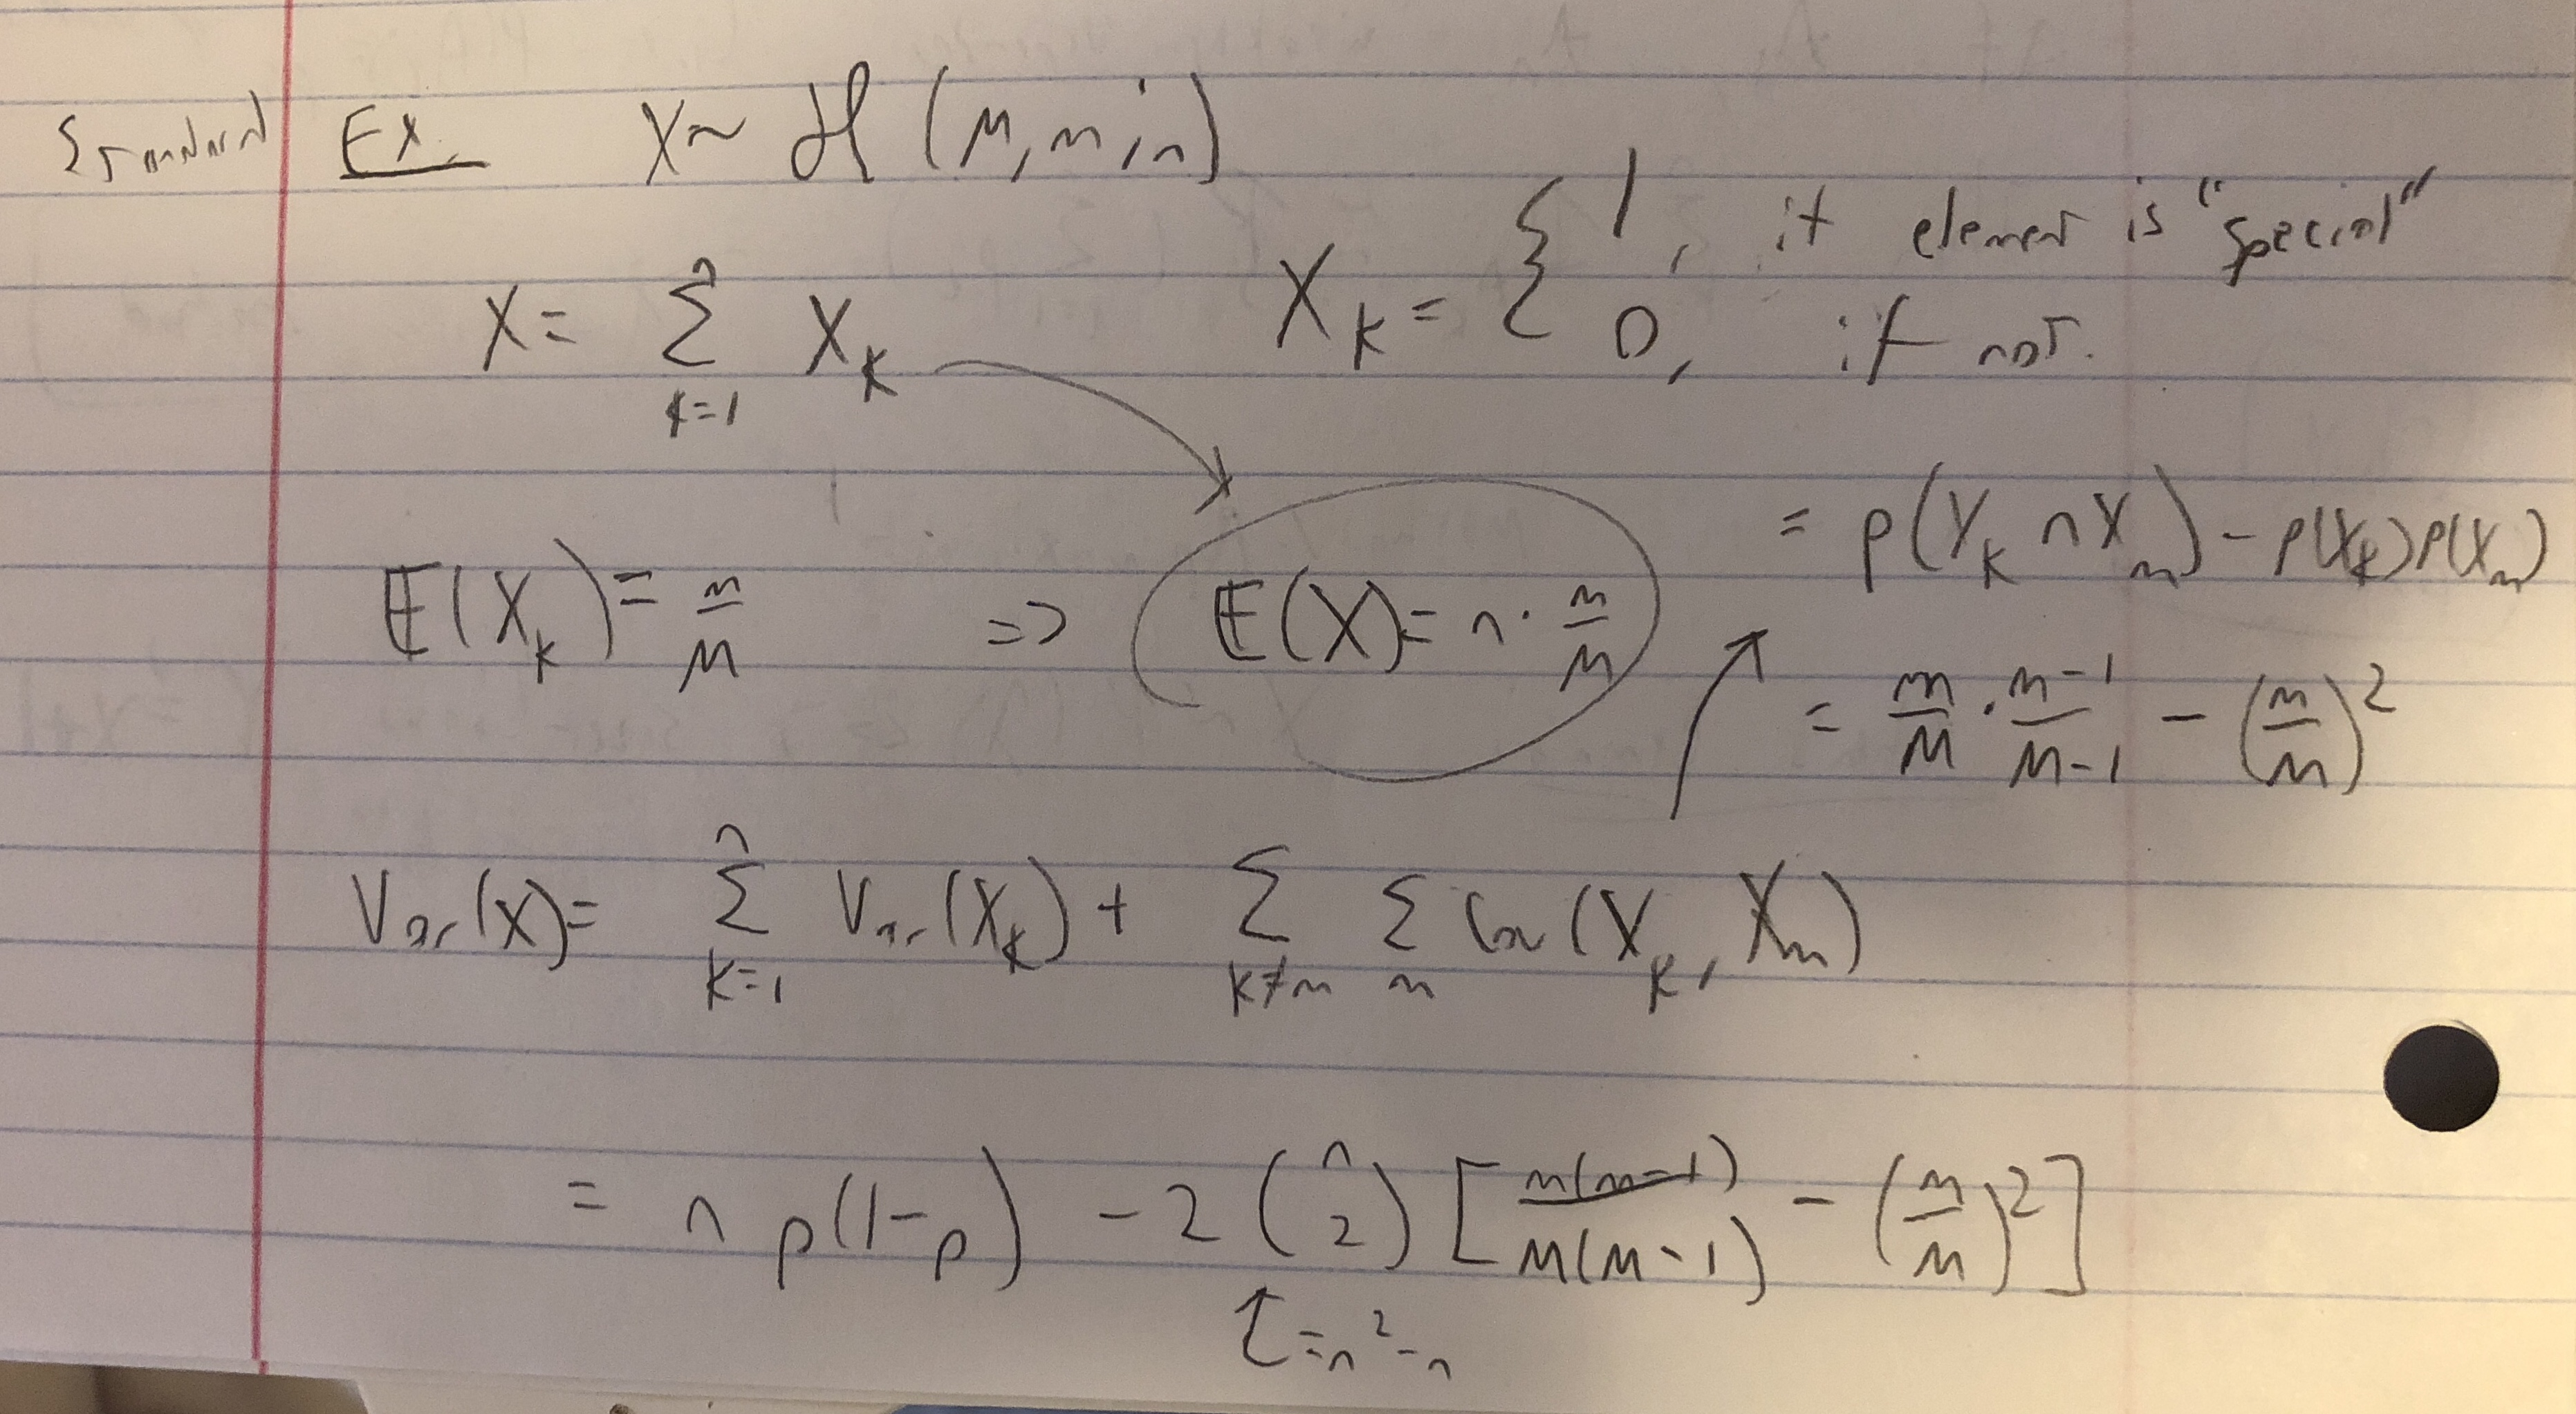
\includegraphics[scale=0.1]{prob_hypergeometric}
\end{proof}

\end{itemize}

\begin{proposition}Let \(X \sim \operatorname{Hypergeometric}(N, M, K)\). Then

\[
\lim_{M, N \to \infty, M/N \to p} \Pr(X=k) \sim \operatorname{Binomial}(K, p)
\]

\end{proposition}

\begin{proof}
\[
\lim_{M, N \to \infty, M/N \to p} p_k(M, N, K) = \lim_{M, N \to \infty, M/N \to p} \frac{\binom{M}{k} \binom{N-M}{K-k}}{\binom{N}{K}}
\]

\[
= \lim_{M, N \to \infty, M/N \to p} \frac{M!(N-M)!/[k!(M-k)!(K-k)!(N-M-K+k)!]}{N!/[K!(N-K)!]}
\]

\[
= \lim_{M, N \to \infty, M/N \to p} \frac{K!}{(K-k)!k!}\cdot \frac{M!(N-M)!(N-K)!}{N!(M-k)!(N-M-K+k)!}
\]

%Note that \( \frac{}{} = \frac{(N-x)!}{(N-x)!} \)

%Note that \((N-K)! = (N-k)!\)

\[
= \lim_{M, N \to \infty, M/N \to p} \binom{K}{k}\cdot \frac{M!/ (M-k)!}{N!/(N-k)!} \cdot \frac{ (N-M)!(N-K)!}{(N-k)! (N-M-(K-k))!}
\]

\[
= \binom{K}{k} \lim_{M, N \to \infty, M/N \to p} \frac{M!/ (M-k)!}{N!/(N-k)!} \cdot \frac{ (N-M)!/  (N-M-(K-k))!}{(N-K+(K-k))!/(N-K)!}
\]

\[
= \binom{K}{k} \lim_{M, N \to \infty, M/N \to p}\prod_{i=0}^{k-1} \frac{M-i}{N-i} \cdot \prod_{j=0}^{K-k-1} \frac{N-M-j}{N-K+1+j}
\]


\[
= \binom{K}{k} \bigg(\frac{M}{N} \bigg)^k \bigg(\frac{N - M}{N} \bigg)^{K-k}
\]

\[
= \binom{K}{k} \bigg(\frac{M}{N} \bigg)^k \bigg(1 - \frac{M}{N} \bigg)^{K-k}=  \binom{K}{k}p^k(1-p)^{K-k} 
\]
\end{proof}


\subsubsection{Indicator Method}

\begin{proposition} If \(\boldsymbol{1}_{A_k}\) is an indicator then

\begin{enumerate}[(a)]

\item

\[
\Cov(\boldsymbol{1}_{A_k}, \boldsymbol{1}_{A_m}) = \E(\boldsymbol{1}_{A_k} \boldsymbol{1}_{A_m}) - \E(\boldsymbol{1}_{A_k}) \E(\boldsymbol{1}_{A_m}) = \Pr(A_k \cap A_m) - \Pr(A_k) \Pr(A_m)
\]

\item

\[
\Var(\boldsymbol{1}_{A_k} ) = \E(\boldsymbol{1}_{A_k} ^2) = \E(\boldsymbol{1}_{A_k} )^2 = \Pr(A_k) - (\Pr(A_k))^2
\]

\end{enumerate}
\end{proposition}

\begin{theorem} \(X\) is independent of \(Y\) if and only if \(X\) is independent of \(\boldsymbol{1}_A\), \(A \in Y\). \end{theorem}

Example problems: 505A Homework 3 problem 9(a)

Worked examples in p. 56 - 59 of Grimmett and Stirzaker 3rd edition.

\subsubsection{Linear transformations of random variables}

\subsubsection{Poisson Paradigm (Poisson approximation for indicator method)}\label{prob.poisson.paradigm}

\begin{theorem} (Theorem 4.12.9, p. 129 of Grimmett and Stirzaker.) Let \(A_i\) be an event. If \(X = \sum_{i=1}^m \boldsymbol{1}_{A_i}\) where \(\boldsymbol{1}_{A_i}\) is an indicator variable for \(A_i\), and the \(A_i\) are only weakly dependent on each other, then 

\[
\text{As } m \to \infty, \ \ X \sim \operatorname{Poisson}(\E(X))
\]

More specifically, let \(B_i\) be \(n\) independent Bernoulli random variables with probabilities \(p_i\). If \(Y = \sum_{i=1}^n B_i\) then 

\[
\text{As } n \to \infty, \ \ Y \sim \operatorname{Poisson} \bigg(\E \bigg(\sum_i B_i \bigg) \bigg) = \operatorname{Poisson}\bigg(\sum_i \E B_i \bigg) = \operatorname{Poisson}\bigg(\sum_i p_i \bigg) 
\]

\end{theorem}

\begin{proof}
Full proof available in Grimmett and Stirzaker, section 4.12, page 129. A justification of the first claim is as follows: if the \(A_i\) are independent and \(\Pr(A_i) = p \ \forall i\), then \(X \sim \operatorname{Binomial}(m, p\)). Then by Proposition \ref{prob.binom.to.poisson}, the result follows. It turns out that this result holds up if the probabilities are not necessarily identical (but all small) and the variables are not necessarily independent (but only weakly dependent).
\end{proof}

\begin{solution} \textbf{Alternative Solution to Exercise \ref {prob.matching} (Matching Problem):} 

Let \(X\) be the number of matches. Let \(P_n = \Pr(X=0)\) given that there are \(n\) people. Let \(Y\) be an indicator variable for the first person who receives their sandwich receiving the correct one. Note that 
\[ P_n = \Pr(X=0) = \Pr(X=0 \mid Y =1) (1/n) + \Pr(X=0 \mid Y=0) (n-1)/n .
\]

Note that if the first person didn't match (\(Y=0\)), we have \(n-2\) people with their hats left, but one of the remaining \(n-1\) people can't get their sandwich because it was taken by the first person. Therefore

\[
\Pr(X=0 \mid Y=0) = \Pr(\{\text{the extra person selects the first person's hat, and the rest of the people pick the wrong hat}\}) 
\]

\[
+ \Pr(\{\text{the extra person does not select the first person's hat, and the rest of the people don't have any matches}\})
\]

\[
= \frac{1}{n-1} \cdot P_{n-2} + P_{n-1}
\]

This yields

\[
P_n = \frac{1}{n} P_{n-2} + \frac{n-1}{n} P_{n-1} \iff P_n - P_{n-1} = - \frac{1}{n}(P_{n-1} - P_{n-2})
\]

which is a recursive formula. Now we seek to find a closed form solution. We have

\[
P_3 - P_2 = - \frac{1}{3} (P_2 - P_1) = - \frac{1}{3!} \iff P_3 = P_2 - \frac{1}{3!} = \frac{1}{2!} - \frac{1}{3!}
\]

\[
P_4 - P_3 = - \frac{1}{4}(P_3 - P_2) = \frac{1}{4!} \iff P_4 = P_3 + \frac{1}{4!} = \frac{1}{2!} - \frac{1}{3!} + \frac{1}{4!}
\]

\[
\vdots
\]

\[
P_n = \frac{1}{2!} - \frac{1}{3!} + \frac{1}{4!} - \ldots + \frac{(-1)^n}{n!} = \sum_{k=0}^n \frac{(-1)^k}{k!} \rightarrow e^{-1} \text{ as } n \to \infty
\]

so we see that for large \(n\) we approximately have \(P_n \sim \operatorname{Poisson}(1)\).

\

Now we consider \(\Pr(X=k)\). Consider a set of \(k\) people who all have matches and no one else matches. The probability that everyone in a set of \(k\) people match is \((n-k)!/n!\). The probability that none of the other \(n-k\) people match is \(P_{n-k}\) per above. Since there are \(\binom{n}{k}\) ways to chose groups of \(k\) people, we have

\[
\Pr(X=k) = \binom{n}{k} \frac{(n-k)!}{n!} \cdot P_{n-k} = \frac{P_{n-k}}{k!} \xrightarrow{n \to \infty} \frac{e^{-1}1^k}{k!}
\]

so again we see that for large \(n\) we approximately have \(P_n \sim \operatorname{Poisson}(1)\).

\end{solution}

\subsubsection{Asymptotic Distributions}

\begin{proposition}
\[
e^x = \lim_{n \to \infty} \bigg( 1 + \frac{x}{n}\bigg)^n
\]
\end{proposition}

\begin{theorem} \label{prob.stirling} \textbf{Stirling's Formula}: 

\[
n! \approx n^ne^{-n} \sqrt{2\pi n}
\]
\end{theorem}

%%%%%%%% Example Problems That Will Likely Appear on Midterm (and Final) %%%%%%%%%%%%%
\subsection{Worked problems}

\subsubsection{Example Problems That Will Likely Appear on Midterm (and Final)}

\begin{enumerate}[(1)]

%%%%%% Midterm 1 Problem 1 %%%%%%%
\item 

\begin{enumerate}[(a)]

\item \textbf{Fall 2011 Problem 1 (same as HW1 problem 5; similar to HW3 problem 2(5).)} Let \(A\) and \(B\) be events such that \( 0 < \Pr(A) < 1\). Show that if \(\Pr(B \mid A) = \Pr(B \mid A^c)\), then \(A\) and \(B\) are independent.

\item Let \(X\) and \(Y\) be two discrete random variables, each taking only two possible values. Show that if \(\E(XY) = \E(X) \E(Y)\) then \(X\) and \(Y\) are independent.

%Show that if the events \(A\) and \(B\) are uncorrelated (\(E(AB) = \E(A)\E(B))\), then they are independent.

\end{enumerate}

\textbf{Solution.}

\begin{enumerate}[(a)]

% 1(a) solution
\item  \(A\) and \(B\) are independent if and only if 

\[
\Pr(A \cap B) = \Pr(A)\cdot\Pr(B)
\]

We know that \[ \Pr(B) = \Pr(B|A)\cdot \Pr(A) + \Pr(B|A^c)\cdot\Pr(A^c)  \]

\[
= \Pr(B|A)\cdot \Pr(A) + \Pr(B|A)\cdot (1 - \Pr(A)) = \Pr(B|A)\cdot \Pr(A) + \Pr(B|A) - \Pr(B|A)\cdot \Pr(A) 
\]

\[
= \Pr(B|A)
\]

Also, we know that since \(\Pr(A) \neq 0\),

\[
\Pr(B|A) = \frac{\Pr(A \cap B)}{\Pr(A)} 
\]

Per above \(\Pr(B|A) = \Pr(B)\), so we have

\[
\Pr(B) = \frac{\Pr(A \cap B)}{\Pr(A)} 
\]

\[
\Pr(A \cap B)= \Pr(A) \cdot \Pr(B)
\]

which is what we were trying to prove. So the answer is \(\boxed{\text{true.}}\)

% 1(b) solution
\item Without loss of generality, let \(X\) and \(Y\) have mass functions

\[
X = \begin{cases}
x_1 & \text{with probability } \Pr(A) \\
x_2 & \text{with probability } \Pr(A^c)
\end{cases} 
\]

\[
Y = \begin{cases}
y_1 & \text{with probability } \Pr(B) \\
y_2 & \text{with probability } \Pr(B^c)
\end{cases} 
\]

Then \(X \indep Y \iff \Pr(A \cap B) = \Pr(A) \Pr(B)\). Let \(\alpha = X - x_2\), \(\beta = Y - y_2\); that is,

\[
\alpha = \begin{cases}
x_1 - x_2 & \text{with probability } \Pr(A) \\
0 & \text{with probability } \Pr(A^c)
\end{cases} 
\]

\[
\beta = \begin{cases}
y_1 - y_2 & \text{with probability } \Pr(B) \\
0 & \text{with probability } \Pr(B^c)
\end{cases} 
\]

Then we have

\begin{itemize}

\item \(\E(\alpha) = (x_1 - x_2) \Pr(A)\)

\item \(\E(\beta) = (y_1 - y_2) \Pr(B)\)

\item \(\E(\alpha \beta) = (x_1 - x_2)(y_1 - y_2) \Pr(A \cap B)\)

\end{itemize}

which we can use to obtain

%\begin{itemize}
%
%\item 

\[
\E(XY) = \E \big[(\alpha + x_2)(\beta + y_2) \big] = \E(\alpha \beta) + y_2 \E(\alpha) + x_2 \E(\beta) + x_2 y_2 
\]

\begin{equation}\label{prob.mid1.b.first}
= (x_1 - x_2)(y_1 - y_2) \Pr(A \cap B) + y_2(x_1 - x_2) \Pr(A) + x_2(y_1 - y_2) \Pr(B) + x_2 y_2
\end{equation}

%\item 

\[
\E(X) \E(Y) = \E(\alpha + x_2) \E(\beta + y_2) = \big[x_2 + (x_1 - x_2) \Pr(A) \big] \big[y_2 + (y_1 - y_2) \Pr(B) \big]
\]

\begin{equation}\label{prob.mid1.b.second}
= x_2 y_2 + x_2(y_1 - y_2)\Pr(B) + y_2(x_1 -x_2) \Pr(A) + (x_1 - x_2)(y_1 - y_2) \Pr(A)\Pr(B)
\end{equation}

%\end{itemize} 

Using \(\E(XY) = \E(X) \E(Y)\), we set (\ref{prob.mid1.b.first}) and (\ref{prob.mid1.b.second}) equal to each other. Canceling terms appearing in both yields

\[
(x_1 - x_2)(y_1 - y_2) \Pr(A \cap B) = (x_1 - x_2)(y_1 - y_2) \Pr(A)\Pr(B) \iff \Pr(A \cap B) = \Pr(A)\Pr(B)
\]

which proves the independence of \(X\) and \(Y\) if \(\E(XY) = \E(X) \E(Y)\).


\end{enumerate}

%\textbf{Fall 2009 Problem 4 (Very similar).} Let \(X\) and \(Y\) be two random variables, both taking only two values. Show that if they are uncorrelated, then they are independent.
%
%\textbf{Solution.} Let \(X\) and \(Y\) have the following pmfs: \(\Pr(X = a) = p, \Pr(X = b) = 1-p; \ \ \ \Pr(Y = c) = q, \Pr(Y = d) = 1  -q \). Suppose \(X\) and \(Y\) are uncorrelated; that is, \(\E(XY) = \E(X)\E(Y)\). Then \(X\) and \(Y\) are independent if \(\Pr(X \cap Y) = \Pr(X) \Pr(Y)\). Since these random variables take on only two values each, this can also be expressed as \( \Pr(X = a \cap Y = c) = \Pr(X = a) \Pr(Y = c)\). 
%
%Begin by defining new variables \(\alpha = X - b\) and \(\beta = Y - d\). Then we have
%
%\[
%\E(\alpha \beta) = \E( (X - b)(Y - d)) = \E(XY) - b \E(Y) -d \E(X) + bd
%\]
%
%\[
%\E(\alpha) \E(\beta) = \E(X-b) \E(Y - d) = \E(X)\E(Y) -b \E(Y) -d \E(X) + bd
%\]
%
%Since by assumption \(\E(XY) = \E(X)\E(Y)\), this yields \(\E(\alpha \beta)  = \E(\alpha) \E(\beta) \). But \(\E(\alpha) = p(a-b) = (a - b) \Pr(X = a)\), \(\E(\beta) = q(c-d) = (c -d) \Pr(Y = c)\), \(\E(\alpha \beta) = (a-b)(c-d)pq = (a - b)(c - d) \Pr(X = a \cap Y = c)\). Therefore
%
%\[
%\E(\alpha \beta)  = \E(\alpha) \E(\beta)  \iff  (a - b)(c - d) \Pr(X = a \cap Y = c) = (a - b) \Pr(X = a) (c -d) \Pr(Y = c)
%\]
%
%\[
%\iff \Pr(X = a \cap Y = c) = \Pr(X = a)  \Pr(Y = c)
%\]
%
%which proves the independence of \(X\) and \(Y\).


%\textbf{Independence Problem 09/24 (number 2 on some qual, likely to be problem 3 on the test)} 
%
%\textbf{Solution.} \(X\) is independent of \(Y\) if and only if \(X\) is independent of \(\boldsymbol{1}_A\), \(A \in Y\). 
%
%\[
%\implies \E(X \mid Y) = \E(X)
%\]
%
%\[
%\E( \E(X \mid Y) \boldsymbol{1}_A) = \E(X \boldsymbol{1}_A) = \E(X) \E(\boldsymbol{1}_A)
%\]
%
%where the last step follows by independence.


%%%%%%%%%%% Midterm 1 Problem 2
\item \textbf{Fall 2013 Qual Problem 1.} Consider a sequence of independent tosses of a pair of fair dice. Compute the probability that the sum 4 will occur before the sum 5.

\textbf{Solution.} Let \(Y_k\) be the outcome of the \(k\)th toss. Let \(X_{k1}\) be the number of the first die on the \(k\)th toss and \(X_{k2}\) be the outcome of the second die. Note that

\[
\Pr(Y_k = 4) = \Pr(X_{k1} = 1 \cap X_{k2} = 3) + \Pr(X_{k1} = 2 \cap X_{k2} = 2) + \Pr(X_{k1} = 3 \cap X_{k2} = 1) = 3 \cdot \frac{1}{36} = \frac{1}{12} 
\]

\[
\Pr(Y_k = 5) = \Pr(X_{k1} = 1 \cap X_{k2} = 4) + \Pr(X_{k1} = 2 \cap X_{k2} = 3) + \Pr(X_{k1} = 3 \cap X_{k2} = 2) 
\]

\[
+ \Pr(X_{k1} = 4 \cap X_{k2} = 1) = 4 \cdot \frac{1}{36} = \frac{1}{9} 
\]

Let \(A_k\) be the event that \(Y_k = 4\) and \(Y_j \neq 4 \text{ or }5 , \  j = 1, \ldots, k-1\). Note that all \(A_k\) are mutually exclusive and 

\[
\Pr(A_k) = \frac{1}{12}\cdot \bigg(1 - \frac{3 + 4}{36} \bigg)^{k-1} = \frac{1}{12} \cdot \bigg( \frac{29}{36} \bigg)^{k-1}.
\]

Then

\[
\Pr(\{\text{roll a 4 before a 5}\}) = \Pr\bigg( \bigcup_{k=1}^\infty A_k \bigg) = \sum_{k=1}^\infty \Pr(A_k) = \frac{1}{12}  \sum_{k=1}^\infty \bigg( \frac{29}{36} \bigg)^{k-1} = \frac{1/12}{1 - 29/36}
\]

\[
= \frac{3}{36 -29} = \boxed{ \frac{3}{7}}
\]

%%%%%%% Midterm 1 Problem 3

\item \textbf{Spring 2013 Problem 1, in notes from 09/21.} Let \(X\) and \(Y\) be random variables such that  \(\E(X \mid Y) = Y, \E(Y \mid X) = X, \E(X^2) < \infty, \E(Y^2) < \infty\). Show that \(\E(X-Y)^2 = 0 \) (or equivalently, show \(\Pr(X = Y) = 1\)).

\textbf{Solution.} 

\[
\E(X-Y)^2 = \E(X^2 - 2XY + Y^2) = \E(X^2) - 2 \E(XY) + \E(Y^2)
\]

\[
\E(XY) = \E( \E(XY\mid Y)) = \E(Y\E(X\mid Y)) = \E(Y \cdot Y) = \E(Y^2)
\]

Also,

\[
\E(XY) = \E(\E(XY \mid X)) = \E(X \E(Y \mid X)) = \E( X \cdot X) = \E(X^2)
\]

Therefore

\[
\E(X-Y)^2 =0
\]


%%%%%%% Midterm 1 Problem 4

\item \textbf{Fall 2016 Problem 4.} Consider a group of \(n \geq 4\) people, among whom are Alice, Bob, Charles, and Diana, standing in a row. Assume that all possible orderings of the \(n\) people are equally likely.

\begin{enumerate}[(a)]

\item Compute the probability that Charles stands somewhere between Alice and Bob. (Note: this does not mean that the three are necessarily adjacent; there can be other people between Alice and Bob.)

\item Compute the probability that Diana stands somewhere between Alice and Bob given that Charles stands somewhere between Alice and Bob.

\item Let \(X\) be the number of people who stand between Alice and Bob. Compute the expected value and the variance of \(X\). (Note: Alice and Bob themselves are not counted in this number.)

\end{enumerate}

%%%%%%% Midterm 1 Problem 4 Solution

\textbf{Solution.}

\begin{enumerate}[(a)]

% Midterm 1 Problem 4 part(a) Solution
\item For this part, \(n\) does not make a difference; all we need to know is the ordering of \(A\), \(B\), and \(C\). This is because conditional on a specific ordering of \(A, B,\) and \(C\), all arrangements of everyone else are equally likely; and conversely, the a particular ordering of \(A\), \(B\), and \(C\) is independent of which three particular slots are made available to them. Examining the permutations of \(A\), \(B\), and \(C\), two of them have \(C\) in the middle, so the answer is \(2/6 = \boxed{1/3}\).

% Midterm 1 Problem 4 part(b) Solution
\item Similarly, the answer is independent of \(n\), so we work with \(n=4\). All possible orderings with Charles between Alice and Bob are as follows:

\[
A C D B, \ A D C B, \ B C D A, \ B D C A, \ A C B D, \ B C A D, \ D A C B,  \ D B C A
\]

The first four of these have Diana between Alice and Bob, so the answer is \(4/8 = \boxed{1/2}\).

% Midterm 1 Problem 4 part(c) Solution
\item Let \(I_k\) be an indicator variable for the event that person \(k\) is between \(A\) and \(B\). By the result from part (a), \(\E(I_k) = 1/3\). Then we have

\[
\Var(I_k) = \E(I_k^2) - \E(I_k)^2 = 1^2 \cdot \Pr(I_k =1) - \frac{1}{9} = \frac{1}{3} - \frac{1}{9} = \frac{2}{9}
\] 

Noting that the four arrangements above with Charles and Diana in between Alice and Bob are the only ones where this will be the case of the \(4! = 24\) possible orderings, we have

\[
\E(I_k I_j) = \frac{4}{24} = \frac{1}{6}
\]

so

\[
\Cov(I_j, I_k) = \E(I_k I_j) - \E(I_i)\E(I_j) = \frac{1}{6} - \frac{1}{9} = \frac{1}{18}
\]

Therefore

\[
\E(X) = \E(\sum_{i=1}^{n-2} I_k) = \sum_{i=1}^{n-2} \frac{1}{3} = \frac{n-2}{3}
\]

\[
\Var(X) = \Var \bigg(\sum_{i=1}^{n-2} I_k \bigg) = \sum_{i=1}^{n-2} \Var(I_k) + 2 \sum_{1 \leq j < k \leq n-2} \Cov(I_j, I_k) = \frac{2(n-2)}{9} + \big[(n-2)^2 - (n-2)\big] \cdot \frac{1}{18} 
\]

\[
= \frac{4(n-2)}{18} + \frac{(n-2)(n-3)}{18} = \boxed{ \frac{(n-2)(n+1)}{18}}
\]


\end{enumerate}

%%%%%%% Midterm 1 Problem 5

\item \textbf{Spring 2015 Problem 2.} A deck of 52 cards is shuffled thoroughly. Someone goes through all 52 cards, scoring 1 point each time 2 cards of the same value are consecutive (that is, when two consecutive cards have the same rank but different suits). For example, the sequence 9H, 8H, 7D, 6C, 7S, 7H, 7C scores 2 points, one for the 7H following the 7S, one for the 7C following the 7H. Let \(X\) be the total score.

\begin{enumerate}[(a)]

\item Compute \(\E(X)\).

\item Compute \(\Pr(X = 39)\). (Note that there are 13 different ranks and you cannot score more than 3 per rank.)

\item In the line below, circle the number that you think is the closest to the value \(\Pr(X=0)\) and briefly explain your choice:

\[
\frac{1}{1000}, \ \ \frac{1}{500}, \ \ \frac{1}{100}, \ \ \frac{1}{50}, \ \ \frac{1}{20}, \ \ \frac{1}{10}, \ \ \frac{1}{5}, \ \ \frac{1}{2}
\]

\end{enumerate}

%%%%%%% Midterm 1 Problem 5 solution

\textbf{Solution.}

\begin{enumerate}[(a)]

% Problem 5(a) Solution
\item Start by assuming the permutation is cyclic (that is, after the last card you go back to the beginning). Let \(Y\) be the number of matches in this situation. Let \(A_i\) be the event that the \(i\)th card is followed by a match. Then \(\Pr(A_i) = 3/51 = 1/17\), so

\[
Y = \sum_{k=1}^{52} \boldsymbol{1}_{\{A_i\}} \implies \E(Y) = \sum_{i=1}^{52} \E(\boldsymbol{1}_{\{A_i\}}) = \sum_{i=1}^{52} \Pr(A_i) = 52 \cdot 1/17 = 52/17
\]

Note that \(\E(Y) = \E(X) + \E(\boldsymbol{1}_{\{A_i\}})\) because if the permutation is cyclic then you have one extra opportunity to mach at the end.

\[
\implies \E(X) = \frac{52}{17} - \frac{1}{17} = \frac{51}{17} = \boxed{3}
\]

% Problem 5(b) Solution
\item \(\Pr(X=39) = \Pr(\{\text{all possible matches occur}\})\), so in this event all cards of the same rank are clustered together. There are 13 clusters of 4 cards, so there are \(13!\) ways to order the clusters and \(4!\) ways to order the cards within each cluster. Therefore

\[
\boxed{
\Pr(X=39) = \frac{13! (4!)^{13}}{52!} }
\]

% Problem 5(c) Solution
\item Because \(A_i\) are only weakly dependent and \(\Pr(A_i)\) is small for all \(A_i\), we can use the Poisson approximation (see Section \ref{prob.poisson.paradigm}); that is, \(X \sim \operatorname{Poisson}(\E(X)) = \operatorname{Poisson}(3)\). Therefore

\[
\Pr(X=0) \approx \frac{e^{-3}\cdot3^0}{0!} = \frac{1}{e^3} \approx \frac{1}{2.8^3} \approx \boxed{\frac{1}{20}}
\]


\end{enumerate}

%%%%%

\end{enumerate}

%%%%%%%%%%% Problems we did in class that professor mentioned %%%%%%%%%%%%


\subsubsection{Problems we did in class that professor mentioned}

\textbf{(Fall 2014 Problem 1) (Variation of Midterm problem 1 above)} Let \(A\) and \(B\) be two events with \(0 < \Pr(A) < 1, \ 0 < \Pr(B) < 1\). Define the random variables \(\xi = \xi(\omega)\) and \(\eta = \eta(\omega)\) by

\[
\xi(\omega) = \begin{cases} 
      5 & \text{ if } \omega \in A \\
      -7 &  \text{ if } \omega \notin A 
   \end{cases}, \ \ \ \ \eta(\omega) = \begin{cases} 
      2 & \text{ if } \omega \in B \\
      3 &  \text{ if } \omega \notin B 
   \end{cases}
\]

True or false: the events \(A\) and \(B\) are independent if and only if the random variables \(\xi\) and \(\eta\) are uncorrelated?

\textbf{Solution.} (\(\implies\)) Suppose \(A\) and \(B\) are independent. Then \(\xi\) and \(\eta\) are uncorrelated if and only if \(\E(\xi \eta ) = \E(\xi) \E(\eta)\). We can write \(\xi = 5 \cdot \boldsymbol{1}_A - 7 \cdot \boldsymbol{1}_{A^c}\) and \(\eta = 2 \cdot \boldsymbol{1}_B + 3 \cdot \boldsymbol{1}_{B^c}\). So we have

\[
\xi \eta = (5 \cdot \boldsymbol{1}_A - 7 \cdot \boldsymbol{1}_{A^c})(2 \cdot \boldsymbol{1}_B + 3 \cdot \boldsymbol{1}_{B^c}) = 10 \cdot \boldsymbol{1}_{A \cap B} +15 \cdot \boldsymbol{1}_{A \cap B^c} - 14 \cdot \boldsymbol{1}_{A^c \cap B} - 21 \cdot \boldsymbol{1}_{A^c \cap B^c}
\]

\[
\implies \E(\xi \eta ) = 10 \Pr(A \cap B) +15\Pr(A \cap B^c) - 14 \Pr(A^c \cap B) - 21\Pr(A^c \cap B^c)
\]

Then

\[
\E(\xi) \E(\eta) = (5 \Pr(A) - 7 \Pr(A^c))(2 \Pr(B) + 3 \Pr(B^c)) 
\]

\[
= 10\Pr(A \cap B) + 15 \Pr(A \cap B^c) - 14 \Pr(A^c \cap B) - 21 \Pr(A^c \cap B^c) = \E(\xi \eta )
\]

where the second-to-last step follows from the independence of \(A\) and \(B\). Therefore \(\eta\) and \(\xi\) are uncorrelated.

(\(\impliedby\)) Now suppose \(\eta\) and \(\xi\) are uncorrelated. Then \(\xi\) and \(\eta\) are independent if and only if \(\Pr(\xi \cap \eta) = \Pr(\xi) \Pr(\eta)\). Define

\[
\alpha(\omega) =  \xi(\omega) + 7 = \begin{cases} 
      12 & \text{ if } \omega \in A \\
      0 &  \text{ if } \omega \notin A 
   \end{cases}, \ \ \ \ \beta(\omega) =  \eta(\omega) - 3 = \begin{cases} 
      -1 & \text{ if } \omega \in B \\
      0 &  \text{ if } \omega \notin B 
   \end{cases}
\]

Then we have

\[
(\alpha \beta)(\omega) = \begin{cases} 
      -12 & \text{ if } \omega \in A \cap B \\
      0 &  \text{ otherwise} 
   \end{cases}
\]

Then

\[
\E(\xi \eta) = \E\big[ (\alpha - 7)(\beta + 3)\big] = \E(\alpha \beta) + 3 \E(\alpha) - 7 \E(\beta) - 21
\]

\[
\E(\xi) \E(\eta) = (\E(\alpha) - 7) (\E(\beta) + 3) = \E(\alpha) \E(\beta) - 7 \E(\beta) + 3 \E(\alpha) - 21
\]

Since by assumption \( \E(\xi \eta)  = \E(\xi) \E(\eta) \), this yields \(\E(\alpha \beta) = \E(\alpha) \E(\beta) \). But

\[
\E(\alpha \beta) = -12 \Pr(A \cap B), \ \ \ \ \ \E(\alpha) \E(\beta) = 12 \Pr(A) (-1) \Pr(B) = -12\Pr(A)\Pr(B)
\]

Therefore \(\Pr(\xi \cap \eta) = \Pr(\xi) \Pr(\eta)\) and \(\xi\) and \(\eta\) are independent.

\begin{exercise}\label{prob.matching} \textbf{Example (Letter/envelope matching problem; sometimes referred to as Montmort's matching problem).} An assistant brings \(n\) sandwiches for \(n\) employees at a company. Each employee ordered a unique sandwich, but unfortunately the assistant forgot to ask that the sandwiches be labeled, so they are all indistinguishable, wrapped in the same paper. The assistant plans to distribute one sandwich to each employee and hope for the best. Let \(X\) be the number of sandwiches that are delivered to the correct person.

\begin{enumerate}[(a)]

\item What is the probability of at least one match; that is, \(\Pr(X \geq 1)\)?

\item What is the probability of \(r\) correct matches?

\item What \(\E(X)\)?

\item What is \(\Var(X)\)?

\end{enumerate}

\end{exercise}

%\textbf{Solution.} 
\begin{solution}

\begin{enumerate}[(a)]
% 2(a)
\item Let \(A_k\) be an indicator variable for the event that sandwich \(k\) is matched to the correct employee. Then

\[
\Pr(X \geq 1) = \Pr\bigg(\bigcup_{k=1}^n A_k \bigg) 
\]

Consider that if there are \(k\) correct matches, there are \(\binom{n}{k}\) sets of \(k\) sandwiches that could be correctly distributed. Also, the probability of a particular set of \(k\) sandwiches being correctly distributed is \((n-k)!/n!\). So we have

\[
\Pr(X = k) = \binom{n}{k} \frac{(n-k)!}{n!} 
\]

Therefore by the Inclusion-Exclusion Principle (Proposition \ref{prob.inex}),

\[
\Pr\bigg(\bigcup_{k=1}^n A_k \bigg)  = \sum_{k=1}^n (-1)^{k-1} \Pr(X=k) = \sum_{k=1}^n (-1)^{k-1} \binom{n}{k} \frac{(n-k)!}{n!}  = \sum_{k=1}^n (-1)^{k-1} \frac{n!}{(n-k)!k!} \frac{(n-k)!}{n!}  
\]

\[
=\sum_{k=1}^n \frac{(-1)^{k-1}}{k!} = \frac{(-1)^{0}}{0!}  -\sum_{k=0}^n \frac{(-1)^{k}}{k!}  = \boxed{1 - \sum_{k=0}^n \frac{(-1)^{k}}{k!}}
\]

As \(n \to \infty\), we have 

\[
1 - \sum_{k=0}^n \frac{(-1)^{k}}{k!} \to 1 - e^{-1} = \boxed{1 - \frac{1}{e}}
\]

%% 2 (b)
\item Clearly there is only one way to match all the sandwiches correctly, so \(\Pr(X = r \mid r = n) = 1/n!\). Also, note that it is impossible to match all but one sandwich, so \(\Pr(X = r \mid r = n -1) = 0\). Only the cases for \(r \leq n - 2\) are nontrivial. Using a similar argument as part (a), we see that for any set of \(m\) sandwiches, the probability that at least one was correctly distributed is 

\[
\Pr\bigg(\bigcup_{k=1}^m A_k \bigg)  = \sum_{k=1}^m (-1)^{k-1} \frac{(n-k)!}{n!}  
\]

and that the probability that \textit{any} set of \(m\) sandwiches contained at least one correct match is
\[
 \sum_{k=1}^m (-1)^{k-1} \binom{n}{k} \frac{(n-k)!}{n!}   = \sum_{k=1}^m (-1)^{k-1} \frac{n!}{(n-k)!k!} \frac{(n-k)!}{n!}  
\]

\[
=\sum_{k=1}^m \frac{(-1)^{k-1}}{k!} = 1 + \sum_{k=2}^m \frac{(-1)^{k-1}}{k!}   = 1 - \sum_{k=2}^m \frac{(-1)^{k}}{k!}
\]




%\[
%\sum_{k=1}^m \frac{(-1)^{k-1}}{k!} = 1 - \sum_{k=0}^m \frac{(-1)^{k}}{k!}
%\]

So for \(m \geq 2\), the probability of \textit{no} correct matches is \(\sum_{k=2}^m \frac{(-1)^{k}}{k!}\) if \(n \geq 2\), and of course \(0\) if \(n = 1\). Therefore the probability of \(r\) matches is the probability of any one set of \(r\) sandwiches all matching and none of the remaining \(n-r\) sandwiches matching times the number of sets of \(r\) sandwiches; that is,

\[
\Pr(X=r \mid r \leq n -2) = \binom{n}{r}  \cdot \frac{(n-r)!}{n!} \cdot \bigg( \sum_{k=2}^{n-r} \frac{(-1)^{k}}{k!} \bigg) = \frac{r!}{(n-r)!r!} \cdot \frac{(n-r)!}{n!} \sum_{k=2}^{n-r} \frac{(-1)^{k}}{k!}  
\]

\[
= \frac{1}{r!} \sum_{k=2}^{n-r} \frac{(-1)^{k}}{k!} 
\]

Therefore we have

\[
\boxed{
\Pr(X=r) = \begin{cases}
\frac{1}{r!} \sum_{k=2}^{n-r} \frac{(-1)^{k}}{k!}  & r \leq n-2 \\
0 & r = n -1 \\
\frac{1}{r!} & r=n
\end{cases}
}
\]

%\[
%\sum_{k=0}^m \frac{(-1)^{k}}{k!}
%\]

% 2(c)
\item 

\[
\E(X) = \E \bigg( \sum_{k=1}^n A_k \bigg) = \sum_{k=1}^n \E(A_k) = \sum_{k=1}^n \Pr(A_k = 1) = n \cdot \frac{1}{n} = \boxed{1}
\]

% 2(d)
\item 

\[
\Var(X) = \E(X^2) - \E(X)^2 
\]

\[
\E(X^2) = \E \bigg(\sum_{k=1}^n A_k \bigg)^2 = \E \bigg(\sum_{k=1}^n A_k^2 + 2 \sum_{1 \leq i < j \leq n} A_i A_j\bigg) = \sum_{k=1}^n \E(A_k^2 ) + 2 \sum_{1 \leq i < j \leq n}  \E(A_i A_j )
\]

Because

\[
\E(A_k^2) = 1^2 \cdot \Pr(A_k = 1) = \frac{1}{n}
\]

\[
\E(A_i A_j) = \Pr(A_j = 1 \cap A_j = 1) = \frac{(n-2)!}{n!}  =  \frac{1}{n(n-1)} = \frac{1}{2} \cdot \binom{n}{2}^{-1}
\]

we have

\[
\E(X^2) = \sum_{k=1}^n \frac{1}{n} + 2 \sum_{1 \leq i < j \leq n}  \frac{1}{n(n-1)} = 1 + 2 \cdot \binom{n}{2} \cdot \frac{1}{2} \cdot \binom{n}{2}^{-1} = 2
\]

\[
\implies \Var(X) = \E(X^2) - \E(X)^2 = 2 - 1 = \boxed{1}
\]

\end{enumerate}

\end{solution}

\textbf{HW3 Problem 2(5).} Verify: \(\E(X \mid Y) = \E(X)\) if \(X\) and \(Y\) are independent.

\textbf{Solution.} \(X\) and \(Y\) are independent if and only if

\[
\Pr(X \cap Y) = \Pr(X)\cdot\Pr(Y) \iff \Pr(X = x \cap Y = y) = \Pr(X = x) \Pr(Y = y)
\]

\[
\iff \Pr(X = x \mid Y = y) \cdot \Pr(Y = y) =  \Pr(X = x) \Pr(Y = y) \iff \Pr(X = x \mid Y = y) = \Pr(X = x)
\]

\[
\implies E(X \mid Y) = \sum_x x \cdot \Pr(X = x \mid Y = y ) = \sum_x x \cdot \Pr(X = x ) = \E(X)
\]




\textbf{HW3 Problem 2 (parts 1 - 4).} Verify:

\begin{enumerate}[(1)]

\item \(\E(\E(X\mid Y)) = \E(X)\)

\item \( \E(g(Y) X \mid Y) = g(Y) \E(X \mid Y) \)

\item \(\Cov ( \E(X \mid Y), Y ) = \Cov(X , Y)\)

\item \(Y\) and \(X - \E(X \mid Y)\) are uncorrelated.

\end{enumerate}

\textbf{Solution.} \begin{enumerate}[(1)]

%1
\item 

\[
\E\big(\E(X\mid Y)\big) = \sum_y \E(X \mid Y) \Pr(Y = y) = \sum_y \bigg[ \sum_x x \cdot \Pr(X = x \mid Y = y) \Pr(Y = y) \bigg]
\]

\[
= \sum_y \bigg[ \sum_x x \cdot \Pr(X = x \cap Y = y) \bigg] = \sum_y \bigg[ \sum_x x \cdot \Pr(Y= y \mid X = x) \cdot \Pr(X = x) \bigg]
\]

\[
= \sum_x \bigg[ x \cdot \Pr(X = x) \cdot \sum_y \big( \Pr(Y= y \mid X = x) \big) \bigg] = \sum_x \bigg[ x \cdot \Pr(X = x) \cdot 1 \bigg]
\]

\[
= \E(X)
\]

%%2
\item 2
%
%%\textbf{double check?}
%
%\[
%\E(g(Y)X \mid Y) = \sum_{y} \sum_x g(y) \cdot x \cdot \Pr(g(Y) = g(y) \cap X = x \mid Y = y) 
%\]
%
%\[
%= \sum_{y} \sum_x g(y) \cdot x \cdot \Pr( X = x \mid Y = y) = \sum_{y}  g(y) \sum_x x \cdot \Pr( X = x \mid Y = y) 
%\]
%
%\[
%= \sum_{y}  g(y) \E(X \mid Y = y)
%\]
%
%
%\[
%= g(Y) \E(X \mid Y)
%\]

%3
\item 

\[
\Cov(\E(X \mid Y) , Y) = \E \bigg( \bigg[\E(X \mid Y) - \E \big(\E(X \mid Y) \big) \bigg] \bigg[Y - \E(Y) \bigg] \bigg)
\]

\[
= \E \bigg( \bigg[\E(X \mid Y) - \E (X) \bigg] \bigg[Y - \E(Y) \bigg] \bigg) = \E \bigg( \E(X \mid Y)Y  - \E (X) Y -  \E(X \mid Y)\E(Y) +  \E(X)\E(Y)  \bigg)
\]

\[
= \E \big( \E(X \mid Y)Y\big)  -  \E (X) \E( Y)  - \E(Y) \E \big( \E(X \mid Y) \big) +   \E(X)\E(Y) = \E \big( \E(X \mid Y)Y\big)  - \E(Y) \E(X)
\]

\[
= \E(XY) - \E(X) \E(Y) = \Cov(X, Y)
\]

%4
\item \(Y\) and \(X  - \E(X \mid Y)\) are uncorrelated if and only if \( \Cov \big(Y, X - \E(X \mid Y) \big) = 0 \iff \E(Y \cdot \big[ X - \E(X \mid Y)\big] ) - \E(Y) \E( X - \E(X \mid Y)) = 0 \).

\[
\E(Y \cdot \big[ X - \E(X \mid Y)\big] ) -  \E(Y) \E( X - \E(X \mid Y))= \E(Y X - Y \E(X \mid Y) ) -  \E(Y) \E( X) +  \E(Y) \E \big( \E(X \mid Y)) \big)
\]

\[
= \E(Y X) - \E\big( Y \E(X \mid Y) \big) -  \E(Y) \E( X)  + \E(Y) \E(X) = \E(YX) - \E(YX) = 0
\]

\end{enumerate}


\textbf{Spring 2018 Problem 2 (did not complete)}

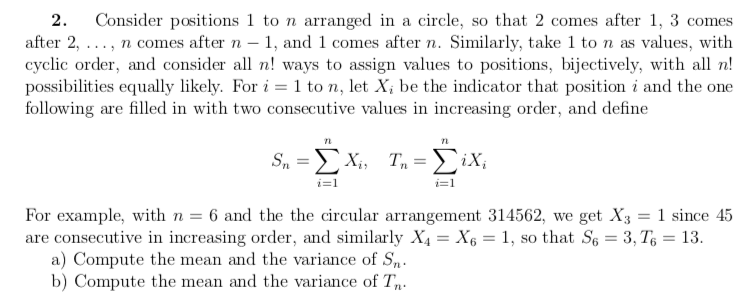
\includegraphics[scale=0.6]{prob_sp18p2}

\textbf{Fall 2008 Problem 2 (HW1 Problem 10).} Consider a lottery with \(n^2\), tickets, of which only \(n\) tickets win prizes. Let \(p_n\) be the probability that, out of \(n\) randomly selected tickets, at least one wins a prize. Compute \(\lim_{n \to \infty} p_n\).

\textbf{Solution.} There are \(\binom{n^2}{n}\) possible sets of \(n\) tickets. The number of these sets that do not contain at least one winner (that is, they only contain members of the \(n^2 - n\) losing tickets) is \(\binom{n^2 - n}{n}\). Therefore the probability of selecting a set of \(n\) tickets that contains at least one winner is

\[
p_n = 1 - \binom{n^2 - n}{n} \bigg/ \binom{n^2}{n} = 1 - \frac{(n^2 - n)!}{n!(n^2 - n - n)!} \bigg/ \frac{(n^2)!}{(n^2 - n)!n!} = 1 - \frac{(n^2 - n)!}{n!(n^2 - 2n)!} \cdot \frac{(n^2 - n)!n!}{(n^2)!}
\]

\[
 = 1 - \frac{(n^2 - n)!}{(n^2 - 2n)!} \cdot \frac{(n^2 - n)!}{(n^2)!} = 1 - \prod_{i=0}^{n-1}(n^2 - n - i)  \bigg/ \prod_{i=0}^{n-1}(n^2 - i) = 1 - \prod_{i=0}^{n-1} \frac{n^2 - n - i}{n^2 - i}
\]

\[
= 1 - \prod_{i=0}^{n-1}\bigg( \frac{n^2 - i}{n^2 - i} -\frac{n}{n^2 - i} \bigg) = 1 - \prod_{i=0}^{n-1}\bigg(1-\frac{n}{n^2 - i} \bigg)
\]

Therefore

\[
\lim_{n \to \infty} p_n = \lim_{n \to \infty} \bigg[ 1 - \prod_{i=0}^{n-1}\bigg(1-\frac{n}{n^2 - i} \bigg) \bigg] = 1 - \lim_{n \to \infty} \prod_{i=0}^{n}\bigg(1-\frac{n}{n^2 - i} \bigg) = 1 - \lim_{n \to \infty} \prod_{i=0}^{n}\bigg(1-\frac{n \cdot \frac{1}{n}}{\frac{n^2}{n} - \frac{i}{n}} \bigg)
\]

\[
= 1 - \lim_{n \to \infty} \prod_{i=0}^{n}\bigg(1-\frac{1}{n - \frac{i}{n}} \bigg) = 1 - \lim_{n \to \infty} \prod_{i=0}^{n}\bigg(1-\frac{1}{n} \bigg) = 1 - \lim_{n \to \infty}  \bigg(1 - \frac{1}{n} \bigg)^n = \boxed{1 - \exp(-1)}
\]

%
%
%
%
%
%
%
%
%
%
%%%%%%%%%%% Problems we did on homework %%%%%%%%%%%%%%%%%%%%%

\subsubsection{Problems we did on homework}

\textbf{Fall 2017 Problem 2 (Homework 3 Problem 6).} An urn contains \(2n\) balls, coming in pairs: two balls are labeled ``1", two balls are labeled ``2", ..., two balls are labeled ``\(n\)". A sample of size \(n\) is taken without replacement. Denote by \(N\) the number of pairs in the sample. Compute the expected value and the variance of \(N\). \textbf{You do not need to simplify the expression for the variance.}

\

%\textbf{From Fall 2017 qual, no solutions to quals that late. Not in solutions to past homeworks online. Seems kind of standard, like I might be able to google.}

%Each ball has one matching partner. Imagine we have \(n/2\) left balls and \(n/2\) right balls. We would like to know the probability 

\textbf{Solution.}  Let \(X_k\) be an indicator variable for both balls labeled \(k\) being in the sample. Note that

\[
\E(X_k) = \Pr(X_k = 1) = \frac{\binom{2n-2}{n-2}}{\binom{2n}{n}} = \left. \frac{(2n-2)!}{(n-2)!n!} \middle/ \frac{(2n)!}{n!n!}  \right. = \frac{(2n-2)!n!}{(2n)!(n-2)!} = \frac{n(n-1)}{2n(2n-1)} = \frac{n-1}{2(2n-1)}
\]

Now since \(N = \sum_{k=1}^n X_k\), we have

\[
\E(N) = \E \bigg( \sum_{k=1}^n X_k \bigg) = \sum_{k=1}^n \E(X_k) = \boxed{\frac{n(n-1)}{2(2n-1)} }
\]

To obtain the variance, note that

\[
\E(N^2) = \E \bigg( \sum_{k=1}^n X_k \bigg)^2 =  \E \bigg( \sum_{k=1}^n X_k^2 + 2\sum_{1 \leq i < j \leq n} X_i X_j \bigg)  = \sum_{k=1}^n \E(X_k^2)   + 2\sum_{1 \leq i < j \leq n} \E(X_i X_j)
\]

Because

\[
\E(X_k^2) = 1^2 \cdot \Pr(X_k = 1) = \E(X_k) = \frac{n-1}{2(2n-1)}
\]

\[
\E(X_i X_j) = \Pr(X_i = 1 \cap X_j = 1) = \frac{\binom{2n-4}{n-4}}{\binom{2n}{n}} = \left. \frac{(2n-4)!}{(n-4)!n!} \middle/ \frac{(2n)!}{n!n!}  \right. = \frac{(2n-4)!n!}{(2n)!(n-4)!} 
\]

\[
= \frac{n(n-1)(n-2)(n-3)}{2n(2n-1)(2n-2)(2n-3)} = \frac{(n-1)(n-2)(n-3)}{2(2n-1)(2n-2)(2n-3)}
\]

we have

\[
\E(N^2) = \sum_{k=1}^n  \frac{n-1}{2(2n-1)}  + 2\sum_{1 \leq i < j \leq n} \frac{(n-1)(n-2)(n-3)}{2(2n-1)(2n-2)(2n-3)} =  \frac{n(n-1)}{2(2n-1)} + 2 \binom{n}{2} \frac{(2n-4)!n!}{(2n)!(n-4)!}  
\]

\[
=\frac{n(n-1)}{2(2n-1)} + \frac{n!}{(n-2)!} \cdot \frac{(2n-4)!n!}{(2n)!(n-4)!} = \frac{n(n-1)}{2(2n-1)} + n(n-1) \cdot  \frac{(n-1)(n-2)(n-3)}{2(2n-1)(2n-2)(2n-3)}
\]

\[
 = \frac{n(n-1)}{2(2n-1)} + \frac{n(n-1)^2(n-2)(n-3)}{2(2n-1)(2n-2)(2n-3)}
\]

\[
\implies \Var(N) = \E(N^2) - \E(N)^2 = \boxed{ \frac{n(n-1)}{2(2n-1)} +  \frac{n(n-1)^2(n-2)(n-3)}{2(2n-1)(2n-2)(2n-3)} - \frac{n^2(n-1)^2}{4(2n-1)^2}}
\]



\textbf{Fall 2017 Problem 3 (HW3 Problem 8---almost full solution)}

Let \(U_1, U_2, \ldots\) be iid random variables, uniformly distributed on \([0, 1]\), and let \(N\) be a Poisson random variable with mean value equal to 1. Assume that \(N\) is independent of \(U_1, U_2, \ldots\) and define 

\[
Y = \begin{cases}
0 & \text{if } N = 0 \\
\underset{{1 \leq i \leq N}}\max U_i & \text{if } N > 0
\end{cases}
\]

Compute the expected value of \(Y\).

%\textbf{Some information in notes from 09/24. Also from Fall 2017 qual, no solutions to quals that late. Feel like might be in notes from 100B. Seems kind of standard, might be able to google.}

\

\textbf{Solution.} Since \(Y\) is a function of \(N\), let \(Y = y(N)\). By the Law of the Unconscious Statistician,

%\[
%\E(Y) = \E( y(N)) = \sum_{n=0}^\infty y(n) \cdot \Pr(N = n) = \sum_{n=1}^\infty \max_{1 \leq i \leq n} U_i \cdot \Pr(N = n) 
%\]

\[
\E(Y) = \E \big( \E( Y \mid N) \big) = \E \big( \E( \max_{1 \leq i \leq N} U_i \mid N = n ) \big) 
\]

Let \( Z_n = \max_{1 \leq i \leq n} U_i  \). The cdf of \(Z_n\) can be calculated as follows:

\[
\Pr(Z_n \leq x) = \Pr(  \max_{1 \leq i \leq n} U_i  \leq x) = \Pr(U_1 \leq x \cap U_2 \leq x \cap \ldots \cap U_n \leq x) = x^n
\]

for \(x \in [0, 1]\). Therefore the pdf of \(Z_n\) is its derivative, \(nx^{n-1}\). So we have

\[
 \E( \max_{1 \leq i \leq N} U_i \mid N = n ) = \E(Z_n) = \int_{0}^1 x n x^{n-1} dx = n \int_0^1 x^n dx = n \frac{x^{n+1}}{n+1} \bigg|_0^1 = \frac{n}{n+1}
\]

Plugging this into the expression for \(\E(Y)\) yields

\[
\E(Y) = \E \big( \E( Y \mid N) \big) = \sum_{n=0}^\infty \frac{n}{n+1} \Pr(N = n) = \sum_{n=1}^\infty \frac{n}{n+1} \frac{\exp(-1)1^n}{n!} 
\]

\[
=\frac{1}{e} \sum_{n=1}^\infty \frac{n + 1  - 1}{(n+1)!} =\frac{1}{e}\bigg(  \sum_{n=1}^\infty \frac{n + 1  }{(n+1)!} -  \sum_{n=1}^\infty \frac{ 1  }{(n+1)!}  \bigg) =\frac{1}{e}\bigg(  \sum_{n=1}^\infty \frac{1  }{n!} -  \sum_{m=2}^\infty \frac{ 1  }{m!}  \bigg) 
\]

\[
= \frac{1}{e} \big[e - 1 - (e - 1 - 1) \big]  = \boxed{\frac{1}{e}}
\]


%\textbf{Spring 2016 Problem 3 (HW3 Problem 5---currently incomplete)} Fix positive integers \(m \leq n\) with \(n > 4\). Suppose \(m\) people sit at a circular table with \(n\) seats, with all \(n\) arrangements equally likely. A seat is called isolated if it isoccupied and both adjacent seats are vacant. Find the mean and variance of the number of isolated seats.
%
%\textbf{Solution.} There are \(\binom{n}{m}\) possible seatings, although only \( \binom{n-1}{m}\) of these are unique up to rotation. Let \(X\) be the number of isolated seats. Clearly if \(m \in \{0,  n-1, n\}\), there can't be any isolated seats, so in these cases, \(\E(X \mid m \in \{0, n-1, n\}) = 0, \ \Var(X  \mid m \in \{0, n-1, n\}) = 0\). Similarly, if \(m = 1\), there must be one isolated seat, so \(E(X \mid m = 1) = 1, \ \Var(X \mid m = 1) = 0\). 
%
%\
%
%Let \(A_i\) be the event that \(i\) people are seated next to at least one more person. If \(m = 2\), \(X = 2\) unless both people are sitting next to each other, in which case we have \(X = 0\). Up to rotation, there are only two ways that these two people can be seated next to each other. So we have
%
% \[
%\E(X \mid m = 2) = 2 \Pr( A_i = 2) = 2 = \frac{2}{\binom{n-1}{2}} = \frac{4(n-3)!}{(n-1)!} = \frac{4}{(n-1)(n-2)} 
%\]

\textbf{Fall 2013 Problem 3/Spring 2011 Problem 2 (HW3 Problem 9; coupon collector problem)} Only parts I didn't do:  Let \(D\) be the event that no box receives more than 1 ball. Fix \(a \in (0,1)\). If both \(n, d \to \infty\) together, what relation must they satisfy in order to have \(\Pr(D) \to a\)?

\textbf{HW3 Problem 9.} Consider \(n\) (different) balls placed at random in \(m\) boxes so that each of \(m^n\) configurations is equally likely.

\begin{enumerate}[(a)]

\item Compute the expected value and the variance of the number of empty boxes.

\item Show that if \(\lim_{m, n \to \infty} m \exp(-n/m) = \lambda \in (0, \infty)\) , then, in the same limit, the number of empty boxes has Poisson distribution with parameter \(\lambda\). 
\item For \(k \geq 1\) such that \(k + 3 \leq m\), define the event \(A_k\) that the boxes \(k, k+1, k+2, k+3\) are empty. Assuming that \(m > 8\), compute \(\Pr(A_1 \cup A_3 \cup A_5)\). How will the answer change if \(m = 8\)?

\item Now imagine that the balls are dropped one-by-one (with each ball equally likely to go into any of the \(m\) boxes, independent of all other balls), and denote by \(N_m\) the minimal number of balls required to fill all the boxes. Compute \(\E(N_m), \Var(N_m)\) and \[ \lim_{m \to \infty} \Pr \bigg( \frac{N_m - m \log m}{m} \leq x \bigg) \]

\item Suppose we instead place an unlimited number of balls into the \(m\) boxes until we have \(k\) consecutive balls land in the same box (it doesn't matter which box). What is the expected number of balls we will drop until this happens?

\end{enumerate}

\textbf{Solution.} \begin{enumerate}[(a)]

% 9a
\item Let \(A_i\) be the event that the \(i\)th box is empty. Let \(\boldsymbol{1}_{A_i}\) be the indicator for \(A_i\). Then \(X = \sum_{i=1}^m \boldsymbol{1}_{A_i}\). 


\[
\E(X) = \E \bigg(\sum_{i=1}^m \boldsymbol{1}_{A_i} \bigg) = \sum_{i=1}^m \bigg( \E \boldsymbol{1}_{A_i} \bigg)  =  \sum_{i=1}^m \Pr(A_i) = \sum_{i=1}^m \bigg( \frac{m-1}{m} \bigg)^n = \boxed{ \frac{(m-1)^n}{m^{n-1}}} 
\]

\[
\Var(X) = \Var \bigg(\sum_{i=1}^m \boldsymbol{1}_{A_i} \bigg) =\sum_{i=1}^m \Var( \boldsymbol{1}_{A_i})  +2\sum_{1 \leq i < j \leq m} \Cov(\boldsymbol{1}_{A_i}, \boldsymbol{1}_{A_j})
\]

\[
\Var(\boldsymbol{1}_{A_i}, \boldsymbol{1}_{A_j}) = \E (\boldsymbol{1}_{A_i} \boldsymbol{1}_{A_i}) - \E (\boldsymbol{1}_{A_i})^2  = \Pr(A_i \cap A_i) - \Pr(A_i)^2 = \bigg( \frac{m-1}{m} \bigg)^n - \bigg( \frac{m-1}{m} \bigg)^{2n} 
\]

\[
\Cov(\boldsymbol{1}_{A_i}, \boldsymbol{1}_{A_j}) = \E (\boldsymbol{1}_{A_i} \boldsymbol{1}_{A_j}) - \E (\boldsymbol{1}_{A_i}) \E( \boldsymbol{1}_{A_j}) = \Pr(A_i \cap A_j) - \Pr(A_i)\Pr(A_j) = \bigg( \frac{m-2}{m} \bigg)^n - \bigg( \frac{m-1}{m} \bigg)^{2n} 
\]

\[
\implies \Var(X) = m \cdot \bigg[  \bigg( \frac{m-1}{m} \bigg)^n - \bigg( \frac{m-1}{m} \bigg)^{2n}  \bigg] + \frac{m!}{(m-2)!} \bigg[\bigg( \frac{m-2}{m} \bigg)^n - \bigg( \frac{m-1}{m} \bigg)^{2n}  \bigg]
\]

\[
= \frac{(m-1)^n}{m^{n-1}} -  \frac{(m-1)^{2n}}{m^{2n-1}} +  (m^2 -m )\bigg[\bigg( \frac{m-2}{m} \bigg)^n - \bigg( \frac{m-1}{m} \bigg)^{2n}  \bigg]
\]

\[
\boxed{
\Var(X) = \frac{(m-1)^n}{m^{n-1}} -  \frac{(m-1)^{2n}}{m^{2n-1}} +  (m - 1)\bigg[ \frac{(m-2)^n}{m^{n-1}}  -  \frac{(m-1)^{2n}}{m^{2n-1}}  \bigg]}
\]



%https://drive.google.com/file/d/0B1RIs0n1fB8Sb1hFTk9OTUptMms/view, page 21 of document

% \textbf{use indicator method, easy.}
%
%Let \(\boldsymbol{1}_{A_i}\) be the event that the \(i\)th box is empty. Then \(X = \sum_{i=1}^m X_{A_i}\). 

% \(X\) be the number of the \(m\) boxes that are nonempty (that is, the \(n\) balls are contained within \(X\) boxes). Then \(\Pr(X \leq k) = \sum_{i=1}^k G_1\big([N-(i-1)]/N \big)\).

% 9b
\item Note that 

\[
X = \sum_{i=1}^m \boldsymbol{1}_{A_i}
\]

and that the \(A_i\) are only weakly dependent on each other, especially as \(m\) and \(n\) increase. Therefore as \(m, n \to \infty\), the Poisson paradigm (see Section \ref{prob.poisson.paradigm}) suggests \(X \sim \operatorname{Poisson}(\E(X))\). We have

\[
\E(X) =  \frac{(m-1)^n}{m^{n-1}}
\]

so

\[
\lim_{n, m \to \infty} \E(X) = \lim_{n, m \to \infty} m \cdot \bigg( \frac{m-1}{m}\bigg)^n = \lim_{n, m \to \infty} m \cdot \bigg( 1 - \frac{1}{m}\bigg)^n = \lim_{n, m \to \infty} m \cdot \bigg[\bigg( 1 - \frac{1}{m}\bigg)^m\bigg]^{n/m}
\]

\[
\approx \lim_{n, m \to \infty} m \cdot \big[e^{-1}\big]^{n/m} = \lim_{n, m \to \infty} m e^{-n/m}
\]

% \textbf{hard, but in notes a little}

%Let \(X_{n, m}\) be the number of empty boxes.

%\[
%\Pr(X = 0) = \Pr \bigg[ \sum_{k=1}^n G_1 \bigg( \frac{n - (k-1)}{n} \bigg) \leq m \bigg]
%\]
%
%\[
%\Pr(X_{n,m} = 1) = \bigg( 1- 1/n\bigg)^m
%\]
%
%\[
%m \bigg[ \bigg(1 - \frac{1}{m} \bigg)^m \bigg]^{n/m} \approx \exp( 
%\]


Using

\[
\lim_{m, n \to \infty} m \exp(-n/m) = \lambda \in (0, \infty)
\]

we have \( \boxed{ X  \sim \operatorname{Poisson}(\lambda) \text{ as } m,n \to \infty }\).

% 9c
\item

% \textbf{solution available online (fall 2013 quals), link here.}

\[
\Pr(A_1 \cup A_3 \cup A_5) = \Pr(A_1) + \Pr(A_3) + \Pr(A_5) - \Pr(A_1 \cap A_3) - \Pr(A_1 \cap A_5) - \Pr( A_3 \cap A_5) + \Pr(A_1 \cap A_3 \cap A_5)
\]

We have

\[
\Pr(A_1) = \Pr(A_3) = \Pr(A_5) = \bigg(  \frac{m-4}{m} \bigg)^n
\]

\[
 \Pr(A_1 \cap A_3) = \Pr( A_3 \cap A_5) =  \bigg(  \frac{m-6}{m} \bigg)^n
\]

\[
\Pr(A_1 \cap A_5) = \Pr(A_1 \cap A_3 \cap A_5) = \bigg(  \frac{m-8}{m} \bigg)^n
\]

Therefore

\[
\Pr(A_1 \cup A_3 \cup A_5) = 3\bigg(  \frac{m-4}{m} \bigg)^n -  2 \bigg(  \frac{m-6}{m} \bigg)^n  = \boxed{ \frac{3(m-4)^n - 2(m-6)^n}{m^n}}
\]

% 9d
\item

% \textbf{some info in notes---"coupon collector problem," maybe use extreme value distribution.}

%https://en.wikipedia.org/wiki/Coupon_collector%27s_problem

\(N_m\) is the minimal number of balls required to fill all the boxes. Let \(T_i\) be the number of balls that have to be dropped to fill the \(i\)th box after \(i - 1\) boxes have been filled. The probability of filling a new box after \(i -1\) boxes have been filled is \( \frac{m - (i - 1)}{m}\). (Note that \(T_1\) should be identically 1 regardless of \(m \geq 1\); this checks out using this expression.) Therefore \(T_i\) has a geometric distribution with \(E(T_i) = \frac{m}{m - (i - 1)}\). Since \(N_m = \sum_{i=1}^m T_i\), we have


\[
\E(N_m) = \E \bigg(  \sum_{i=1}^m T_i   \bigg) =  \sum_{i=1}^m \E( T_i )  =  \sum_{i=1}^m \frac{m}{m - (i - 1)} = \boxed{m  \sum_{i=1}^m \frac{1}{i }}
\]

Because the \(T_i\) are independent, we have

\[
\Var(N_m) = \Var \bigg(  \sum_{i=1}^m T_i   \bigg) =  \sum_{i=1}^m \Var( T_i )  =  \sum_{i=1}^m \left. \bigg( 1 -  \frac{m - (i - 1)}{m} \bigg) \middle/ \bigg( \frac{m - (i - 1)}{m} \bigg)^2 \right.
\]

\[
=  \sum_{i=1}^m  \frac{  i - 1}{m} \cdot \bigg( \frac{m}{m - (i - 1)} \bigg)^2 = \boxed{  m\sum_{i=1}^m  \frac{ i - 1}{[m - (i - 1)]^2} }
\]

%\[
%\Var(N_m) = \Var \bigg(  \sum_{i=1}^m X_i   \bigg) =  \sum_{i=1}^m \Var( X_i )  =   \sum_{i=1}^m \E(X_i^2) - \E(X_i)^2
%\]

Finally, to find

\[
\lim_{m \to \infty} \Pr \bigg( \frac{N_m - m \log m}{m} \leq x \bigg) 
\]

begin by noting that we can also express \(N_m\) as 

\[
\Pr(N_m \leq k) = \Pr \big( X_{m, k} = 0 \big)
\]

where \(X_{m, k}\) is defined as \(X\) is in part (b) with \(k\) being the number of balls that have been dropped so far, \(k \in \mathbb{N} \geq m\). (For \(k < m\), \(\Pr(N_m \leq k) = 0\).)

\

Again, let \(A_{i,k}\) be the event that the \(i\)th box is empty after dropping \(k\) balls. Then because \(X_{m, k} = \sum_{i=1}^m \boldsymbol{1}_{A_{i,k}}\) and the \(A_{i,k}\) are only weakly dependent on each other (especially as \(m\) becomes large), the Poisson paradigm (see Section \ref{prob.poisson.paradigm}) again suggests that as \(m \to \infty\), \(X_{m, k} \sim \operatorname{Poisson}(\lambda_k)\) where \(\lambda_k = \E(X_{m,k})\) is defined as above. Therefore we have

\[
\lim_{m \to \infty} \Pr \bigg( \frac{N_m - m \log m}{m} \leq x \bigg) = \lim_{m \to \infty} \Pr \big( N_m \leq xm + m \log    m\big) = \lim_{m \to \infty} \Pr \big( X_{m, {xm + m \log    m}} 
\]

\[
= 0) \approx \frac{\exp(-\lambda_ {xm + m \log    m}) \cdot \lambda_ {xm + m \log    m}^0}{0!} = \exp \big(-\lambda_ {xm + m \log    m} \big)
\]



And we have

\[
\lambda_ {xm + m \log    m} = \lim_{m \to \infty} m \exp \bigg(-\frac{xm + m \log    m}{m} \bigg) = \lim_{m \to \infty} m \exp \big(-x -  \log    m\big)   = \lim_{m \to \infty} m/m \exp (-x ) 
\]



\[
 = \exp(-x)
\]

which yields

\[
\boxed{
\lim_{m \to \infty} \Pr \bigg( \frac{N_m - m \log m}{m} \leq x \bigg)  = \exp( \exp(-x))}
\]



%begin by noting that as \(m \to \infty\), the \(X_i\) become approximately i.i.d., which means that \\ \(N_m \sim \operatorname{Negative Binomial}(, ) \).

%\[
%\lim_{m \to \infty} \Pr \bigg( \frac{N_m - m \log m}{m} \leq x \bigg) = \lim_{m \to \infty} \Pr \bigg(  \frac{1}{m} \sum_{i=1}^m T_i   \leq x + \log m\bigg)
%\]

% Part (e) 
\item Let \(N = N_k\) be the number of balls that are dropped until \(k\) consecutive balls land in the same box, and likewise for \(N_{k-1}\). Suppose we have already observed \(k-1\) consecutive outcomes (of any kind) in \(N_{k-1} \) trials. Then we finish on the next term (by having another consecutive outcome) with probability \(1/m\). Otherwise we have a different outcome and then repeat the same process again. So we have

\[
\E(N_k \mid N_{k-1} ) = N_{k-1} + 1 \cdot \frac{1}{m} + \E(N_k) \cdot \bigg(1 - \frac{1}{m} \bigg)
\]

Therefore

\[
\E(N) = \E(N_k) = \E \big[ \E(N_k \mid N_{k-1} )\big] = \E(N_{k-1}) + \frac{1}{m} + \bigg(1 - \frac{1}{m} \bigg) \E(N_k)
\]

\[
\iff \frac{1}{m} \E(N_k) = \E(N_{k-1}) + \frac{1}{m} \iff \E(N_k) = m \E(N_{k-1}) + 1
\]

We have a recursive formula. Note that \(\E(N_1) = 1\) because the number of trials until there is 1 consecutive outcome of any kind is simply 1. We can then calculate as follows:

\[
\E(N_2) = m \E(N_{2-1}) + 1 = m + 1
\]

\[
\E(N_3) = m \E(N_{3-1}) + 1 = m(m + 1) + 1 = 1 + m + m^2
\]

\[
\E(N_4) = m \E(N_{4-1}) + 1 = m(1 + m + m^2) + 1 = 1 + m + m^2 + m^3
\]

\[
\vdots
\]

\[
\E(N_k) = \sum_{i=0}^{k-1} m^i = \frac{1 \cdot (1-m^{k})}{1 - m} = \boxed{\frac{m^k -1}{m-1}}
\]


\end{enumerate}


\textbf{Fall 2012 Problem 1 (HW2 Problem 10/HW 1 Problem 9)} Only part I didn't do: Find the mean and variance of \(S_n = X_1 + \ldots + X_n\), the total number of white balls added to the urn up to time \(n\).

\textbf{HW1 Problem 9.} An urn contains \(b\) black and \(w\) white balls. At each step, a ball is removed from the urn at random and then put back together with one more ball of the same color. Compute the probability \(p_n\) to get a black ball on step \(n, n \geq 1\).

\textbf{Solution.} \textbf{Step 1:}

\[
p_1 = \frac{b}{b+w}
\]

\

\textbf{Step 2:} We need to separately consider the cases where a black ball was selected on step 1 (with probability \(p_1\)) or a white ball (with probability \(1 - p_1\)).

\[
p_2 = p_1 \cdot \frac{b + 1}{b + w + 1} + (1 - p_1) \cdot \frac{b}{b + w + 1} = p_1 \bigg(\frac{b + 1}{b + w + 1} -  \frac{b}{b + w + 1} \bigg) + \frac{b}{b + w + 1}
\]

\[
= p_1\bigg( \frac{1}{b + w + 1} + \frac{1}{p_1}\frac{b}{b + w + 1} \bigg) = p_1\bigg( \frac{1}{b + w + 1} + \frac{b + w}{b}\frac{b}{b + w + 1} \bigg) 
\]

\[
= p_1 \bigg(\frac{b + w + 1}{b + w + 1} \bigg) = p_1
\]

%\frac{p_1 b + p_1 + b - p_1 b}{b + w + 1}

%\[
%= \frac{1}{b + w + 1} \bigg(\frac{b}{b+w} \cdot (b+1) + \frac{w}{b+w} \cdot b \bigg) = \frac{b(b + 1 +w)}{(b + w + 1)(b + w)}
%\]

\[
\implies p_2 = p_1 =  \frac{b}{b+w}
\]

\textbf{Step 3:} Regardless of the previous steps, there are now \(b + w + 2\) balls in the urn. Since we know that \(p_1 = p_2\), the probability that we have selected \(k\) black balls so far (and thus, the probability that there are currently \(b + k\) black balls in the urn) is given by

\[
\Pr(k \text{ balls chosen in first 2 rounds}) = \binom{2}{k}p_1^k(1 - p_1)^{2 - k} = \binom{2}{k} \bigg(\frac{b}{b+w} \bigg)^k \bigg(\frac{w}{b+w} \bigg)^{2 - k}
\]

\[
= \binom{2}{k}\frac{b^k w^{2-k}}{(b+w)^2} 
\]

for \(k \in \{0, 1, 2\}\). Given that we have selected \(k\) black balls so far, the probability of selecting a black ball this time is \(\frac{b + k}{b + w + 2}\). Therefore the probability of selecting a black ball this round is

\[
p_3 = \sum_{k=0}^2 \binom{2}{k}\frac{b^k w^{2-k}}{(b+w)^2} \frac{b + k}{b + w + 2} = \frac{1}{(b+w+2)(b+w)^2} \sum_{k=0}^2 \binom{2}{k} (b+k)b^kw^{2-k}
\]

\[
= \frac{1}{(b+w+2)(b+w)^2} \bigg( \binom{2}{0}bw^2 + \binom{2}{1}(b+1)bw + \binom{2}{2}(b+2)b^2 \bigg)
\]

\[
= \frac{bw^2 + 2(b+1)bw + (b+2)b^2}{(b+w+2)(b+w)^2} = \frac{b}{b+w} \bigg(\frac{w^2 + 2bw + 2w + b^2 + 2b}{b^2 + bw + 2b + wb + w^2 + 2w}\bigg)
\]

\[
=\frac{b}{b+w} \bigg( \frac{w^2 + 2bw + 2w + b^2 + 2b}{b^2 + 2bw + 2b + w^2 + 2w} \bigg) = \frac{b}{b+w} = p_1
\]

\

There seems to be a clear pattern here. Let's find the general formula by induction.

\

\textbf{Step \(n + 1\):} Assume that the probability of choosing a black ball on steps \(1, 2, \dots, n\) was \( \frac{b}{b+w}\) each time.

(a bunch of boring stuff, then it worked.)

\textbf{HW2 Problem 10.} Random variables \((X_1, \ldots, X_n)\) are called \textit{exchangeable} if \(\Pr(X_1 = x_1, \ldots, X_n = x_n) = \Pr(X_{\tau(1)} = x_1, \ldots, X_{\tau(n)} = x_n) \) for all real numbers \(x_1, \ldots, x_n\) and every permutation \(\tau\) of the set \(\{1, \ldots, n\}\). In the setting of Problem 9 from Homework 1, let \(X_k = 1\) if a white ball is drawn on step \(k\), and \(X_k =0\) otherwise. Show that the random variables \(X_1, \ldots, X_n\) are exchangeable for every \(n \geq 2\).

\textbf{Solution.} For \(n =2\): There are two cases which we must show are equal to show exchangeability:

\[
\Pr(X_1 = 0, X_2 = 1) = \Pr(X_1 = 1, X_2 = 0)
\]

First,

\[
\Pr(X_1 = 0, X_2 = 1) = \Pr(\text{black first}) \Pr(\text{white second} \mid \text{black first}) = \bigg( \frac{b}{b+w}\bigg) \bigg( \frac{w}{b+w+1}\bigg)
\]

\[
\bigg( \frac{w}{b+w}\bigg) \bigg( \frac{b}{b+w+1}\bigg)= \Pr(X_1 = 1, X_2 = 0)
\]

which proves exchangeability for \(n=2\). In the general case, we seek to show that \(X_1, \ldots, X_n\) are exchangeable. That is, in all \(n +1\) unordered sets \(\mathbb{X}_k = \{x_{1k}, x_{2k}, \ldots, x_{nk} \mid x_{ik} \in \{0, 1\}, \sum_i x_{ik} = k\}\), in all \(\binom{n}{k}\) permutations of \(\mathbb{X}_k\), 

\[
\Pr(\mathbb{X}_{kj} = \Pr(\mathbb{X}_{kj'}
\]

where \(j\) and \(j'\) denote different permutations of \(\mathbb{X}_k\). That is,

\[
\Pr(X_1 = x_{1k}, X_2 = x_{2k}, \ldots, X_n = x_{nk}) = \Pr(X_{j_1} = x_{1k}, X_{j_2} = x_{2k}, \ldots, X_{j_n} = x_{nk})
\]

where \(j_1, j_2, \ldots, j_n\) index the permuted variables. Consider \(\mathbb{X}_{kj^*}\) where all \(k\) white balls are chosen first and all \(n -k\) black balls are chosen last. We have

\[
\Pr(\mathbb{X}_{kj^*}) = \prod_{i=1}^k \bigg( \frac{w+i-1}{b+w+i-1}\bigg) \cdot \prod_{i=k+1}^n \bigg( \frac{b+i-k-1}{b+w+i-1} \bigg) 
\]

\[
= \prod_{i=1}^n \bigg( \frac{1}{b+w+i-1} \bigg) \cdot \bigg[ \prod_{i=1}^k (w+i-1) \prod_{i=k+1}^n (b+i-k-1) \bigg] = \prod_{i=1}^n \bigg( \frac{1}{b+w+i-1} \bigg) \cdot \bigg[ \prod_{i=1}^k (w+i-1) \prod_{i'=1}^{n-k} (b+i'-1) \bigg]
\]

It is easy to see that the leftmost product will always equal the product of the denominators, regardless of the permutation, since one ball is added to the urn after every draw. Similarly, regardless of permutation, the numerator of the probability of drawing the \(i\)th white ball will always equal \(w +i-1\), the number of white balls already in the urn. Likewise, the numerator of the probability of drawing the \(i'\)th black ball is always \(b +i'-1\). Because multiplication is commutative, all permutations of these numbers will have equal products. Therefore \( \Pr(\mathbb{X}_{kj^*})  = \Pr(\mathbb{X}_{kj}\) for all \(k\). That is, 

\[
\Pr(X_1 = x_1, \ldots, X_n = x_n) = \Pr(X_{\tau(1)} = x_1, \ldots, X_{\tau(n)} = x_n) 
\]

for all \((x_1, \ldots, x_n) \in \mathbb{R}^n\), all \(n \in \mathbb{Z} \) such that \(n \geq 2\), all permutations \(\tau\). 

\textbf{Homework 2 Problem 2.} Consider the function

\[
f(x) = \begin{cases}
C(2x - x^2) & 0 < x < 2 \\
0 & \text{otherwise}
\end{cases}
\]

\begin{enumerate}[(a)]

\item Could \(f\) be a distribution function? If so, determine \(C\).

\item Could \(f\) be a probability density function? If so, determine \(C\).

\end{enumerate}

\textbf{Solution.} 

\begin{enumerate}[(a)]

\item If \(f\) is a distribution function, \(\lim_{x \to -\infty} f(x) = 0\), \(\lim_{x \to \infty} f(x) = 1\), and \(f'(x) \geq 0 \ \forall \ x \in \mathbb{R}\). \(f\) clearly does not meet the second or third conditions and is therefore \boxed{\text{not a distribution function.}}

\item If \(f\) is a density function then \(\int_{-\infty}^{\infty} f(x) dx = 1\) and \(f(x) \geq 0 \ \forall x \in \mathbb{R}\). 

\[
\int_{-\infty}^{\infty} f(x) dx = \int_{0}^2 C(2x - x^2) dx = C \bigg[ x^2 - \frac{x^3}{3}\bigg]_0^2 = C \bigg( 4 - \frac{8}{3} - 0\bigg) = C \cdot \frac{4}{3} 
\]

\[
= 1 \iff C = \frac{3}{4}
\]

Next we check that \(f\) is always nonnegative. It equals zero except on \((0, 2)\). 

\[
\frac{3}{4}(2x -  x^2) \geq 0 \iff x(2 - x) \geq 0 \iff x \in (0, 2)
\]

Therefore \(f\) is nonnegative \(\forall x \in \mathbb{R}\), so \boxed{f \text{ is a probability density function if } C = \frac{3}{4}.}

\end{enumerate}

%%%%%%%%% Homework 1 Problem 8 %%%%%%%%%%%%

\textbf{HW1 Problem 8.} Two people, \(A\) and \(B\), are involved in a duel. The rules are simple: shoot at each other once; if at least one is hit, the duel is over, if both miss, repeat (go to the next round), and so on. Denote by \(p_A\) and \(p_B\) the probabilities that \(A\) hits \(B\) and \(B\) hits \(A\) with one shot, and assume that that hitting/missing is independent from round to round. Compute the probabilities of the following events: (a) the duel ends and \(A\) is not hit; (b) the duel ends and both are hit; (c) the duel ends after round number \(n\); (d) the duel ends after round number \(n\) GIVEN that \(A\) is not hit; (e) the duel ends after \(n\) rounds GIVEN that both are hit; (f) the duel goes on forever.

\textbf{Solution.} \begin{enumerate}[(a)]

% 8a
\item Let \(A_k\) denote the event that the duel is ended by \(A\) shooting \(B\) in the \(k\)th round (with neither person being shot in the first \(k - 1\) rounds). Note that \( \{A_k | k = 1, 2, \ldots\}\) are all mutually exclusive. Therefore the probability of the duel ending without \(A\) being hit is \(\sum_{k=1}^\infty A_k\). Because the probabilities in each round are constant and independent, 

\[
A_k = (1 - p_A)^{{k-1}}p_A(1 - p_B)^{k}
\]

So the probability that the duel ends and \(A\) is not hit is

\[
\sum_{k=1}^\infty A_k = \sum_{k=1}^\infty (1 - p_A)^{{k-1}}p_A(1 - p_B)^{k} = p_A (1 - p_B)\sum_{k=1}^\infty (1 - p_A)^{{k-1}}(1 - p_B)^{k-1} 
\]

This is an infinite geometric series. Since the ratio \((1 - p_A)(1 - p_B)\) has absolute value less than 1, the sum can be calculated.

\[
\sum_{k=1}^\infty A_k = p_A (1 - p_B) \cdot \frac{1}{1 - (1 - p_A)(1 - p_B)} = \frac{p_A (1 - p_B) }{p_A + p_B - p_Ap_B} = \boxed{\frac{p_A (1 - p_B) }{p_A(1 - p_B) + p_B}}
\]

% 8b
\item Similar to part (a). Let \(C_k\) denote the event that the duel is ended with both players being shot in the \(k\)th round (with neither person being shot in the first \(k - 1\) rounds). Again, \( \{C_k | k = 1, 2, \ldots\}\) are all mutually exclusive, so the probability of the duel ending in these circumstances is \(\sum_{k=1}^\infty C_k\). We have

\[
C_k = (1 - p_A)^{{k-1}}p_A(1 - p_B)^{k-1}p_B
\]

\[
\sum_{k=1}^\infty C_k = \sum_{k=1}^\infty (1 - p_A)^{{k-1}}p_A(1 - p_B)^{k-1}p_B = p_A p_B\sum_{k=1}^\infty (1 - p_A)^{{k-1}}(1 - p_B)^{k-1} 
\]

\[
= p_A p_B \cdot \frac{1}{1 - (1 - p_A)(1 - p_B)} = \boxed{ \frac{p_A p_B }{p_A + p_B - p_Ap_B} }
\]

Note that this value is less than the answer from part (a) if \(p_B < \frac{1}{2}\) and greater if \(p_B > \frac{1}{2}\)

% 8c
\item Let \(B_k\) denote the event that the duel is ended by \(B\) shooting \(A\) in the \(k\)th round (with neither person being shot in the first \(k - 1\) rounds), with

\[
B_k = (1 - p_A)^{{k}}p_B(1 - p_B)^{k-1}
\]

Let \(A_k\) and \(C_k\) be defined as above. Note that \(\{A_k | k = 1, 2, \ldots\} , \{B_k | k = 1, 2, \ldots\}, \{C_k | k = 1, 2, \ldots\}\) are all mutually exclusive, and that the event that the duel ends in round \(n\) is \(\{A_n \cup B_n \cup C_n\}\). So the probability of the duel ending in round \(n\) is

\[
\Pr(A_n \cup B_n \cup C_n) = \Pr(A_n) + \Pr(B_n) + \Pr(C_n) 
\]

\[
= (1 - p_A)^{n-1}p_A(1 - p_B)^{n} + (1 - p_A)^{{n}}p_B(1 - p_B)^{n-1} + (1 - p_A)^{{n-1}}p_A(1 - p_B)^{n-1}p_B
\]

\[
= (1 - p_A)^{n-1}(1 - p_B)^{n-1} \big[p_A(1 - p_B) + (1 - p_A)p_B + p_Ap_B \big]
\]

\[
= \boxed{(1 - p_A)^{n-1}(1 - p_B)^{n-1} (p_A + p_B - p_Ap_B )}
\]

% 8d
\item Let \(A_k\), \(B_k\), \(C_k\) be defined as above. The event that the duel ends at round \(n\) without \(A\) being hit is given by \(\{ A_n\} \). 

\[
\Pr(A_n) = \boxed{(1 - p_A)^{{n-1}}p_A(1 - p_B)^{n}}
\]

% 8e
\item Let \(A_k\), \(B_k\), \(C_k\) be defined as above. The event that the duel ends at round \(n\) with both players being hit is given by \(\{ C_n\} \). 

\[
\Pr(C_n) = \boxed{(1 - p_A)^{{n-1}}p_A(1 - p_B)^{n-1}p_B}
\]

% 8e
\item Let \(A_k\), \(B_k\), \(C_k\) be defined as above. The probability that the duel never ends is equal to 1 - the probability that the duel ends at some point, which is  \(\{A_k | k = 1, 2, \ldots\} \cup \{B_k | k = 1, 2, \ldots\} \cup \{C_k | k = 1, 2, \ldots\}\). Since all of these events are mutually exclusive, we have

\[
1 - \Pr(\{A_k | k = 1, 2, \ldots\} \cup \{B_k | k = 1, 2, \ldots\} \cup \{C_k | k = 1, 2, \ldots\}) = 1 - \sum_{k = 1}^\infty \big(A_k + B_k + C_k\big)
\]

\[
= 1 - \sum_{k=1}^\infty \big( (1 - p_A)^{{k-1}}p_A(1 - p_B)^{k} + (1 - p_A)^{{k}}p_B(1 - p_B)^{k-1} + (1 - p_A)^{{k-1}}p_A(1 - p_B)^{k-1}p_B \big)
\]

\[
= 1 -   \big[p_A(1 - p_B) + (1 - p_A)p_B + p_Ap_B \big] \sum_{k=1}^\infty (1 - p_A)^{k-1}(1 - p_B)^{k-1} 
\]

\[
=  1 -  \big[ p_A1 - p_A p_B) + p_B - p_A)p_B + p_Ap_B \big] \cdot \frac{1}{1 - (1 - p_A)(1 - p_B)}
\]

\[
=1 -  \frac{p_A - p_Ap_B + p_B - p_Ap_B + p_Ap_B}{p_A + p_B - p_Ap_B} = 1 -  \frac{p_A + p_B - p_Ap_B}{p_A + p_B - p_Ap_B} = \boxed{0}
\]

\end{enumerate}


%%%%%%%% Homework 1 Problem 1 %%%%%%%%%%

\textbf{Homework 1 Problem 1.} 

\begin{enumerate}[(I)]

\item Seven different gifts are distributed among 10 children. How many different outcomes are possible if every child can receive (a) at most one gift, (b) at most two gifts, (c) any number of gifts?

\item Answer the same questions if the gifts are identical (but the children are still different).

\end{enumerate}

\textbf{Solution.} 

\begin{enumerate}[(I)]

\item

\begin{enumerate}[(a)]

% 1 (I) (a)
\item \(\binom{10}{7}7! = \boxed{604,800}\)

% 1 (I) (b)
\item Clearly all outcomes that satisfy part (I)(a) also satisfy these conditions, so we start with \(\binom{10}{7}7! = 604,800\) possible outcomes. In addition, the following outcomes are possible:

\begin{enumerate}[(i)]

\item \textbf{A set of 6 children receive gifts; one child receives two gifts.} There are \(\binom{10}{6}\) ways to pick a group of 6 children to receive the gifts. Next, there are \(\binom{6}{1} = 6\) ways to choose which child receives two gifts. Finally, there are \(7!/2!\) unique ways to distribute the gifts among the children once a particular partition is chosen (since order matters for all of the gifts except for the two that are received by the same child). 

\item \textbf{A set of 5 children receive gifts; two children receive two gifts.} There are \(\binom{10}{5}\) ways to pick a group of 5 children to receive the gifts. Next, there are \(\binom{5}{2}\) ways to choose which of these children receive one gift and which receive two. Finally, there are \(7!/(2!2!)\) unique ways to distribute the gifts among the children once a particular partition is chosen (since order matters for all of the gifts except for the two batches of two gifts that are received by the same child). 

(Note that without the restriction that a child can receive at most two gifts, another possibility is that 1 child could receive 3 gifts, but that wouldn't work in this case.)

\item \textbf{A set of 4 children receive gifts; three children each receive two gifts.} There are \(\binom{10}{4}\) ways to pick a group of 4 children to receive the gifts. Next, there are \(\binom{4}{3} = 4\) ways to choose which of these children receive one gift and which receive two. Finally, there are \(7!/(2!2!2!)\) unique ways to distribute the gifts among the children once a particular partition is chosen (since order matters for all of the gifts except for the three batches of two gifts that are received by the same child). 

(Again, there are other possibilities for 4 children to receive 7 gifts, but none that satisfy the condition that no child receives more than 2 gifts.)

\end{enumerate}

Clearly each of these outcomes are mutually exclusive. Therefore the answer is

\[
\binom{10}{7}7! + \binom{10}{6} \cdot \binom{6}{1} \cdot \frac{7!}{2!} + \binom{10}{5} \cdot \binom{5}{2} \cdot \frac{7!}{2!2!} + \binom{10}{4} \cdot \binom{4}{3} \cdot \frac{7!}{2!2!2!} 
\]

\[
= 7!\cdot \bigg(\frac{10!}{3!} + \frac{10!}{6!4!}\cdot6 \cdot \frac{1}{2} + \frac{10!}{5!5!} \cdot \frac{5!}{3!2!} \cdot \frac{1}{4} + \frac{10!}{4!6!} \cdot \frac{4!}{3!} \cdot \frac{1}{8}  \bigg) 
\]

\[
= 7!10!\cdot \bigg(\frac{1}{3!} + \frac{1}{6!4!}\cdot\frac{6}{2} + \frac{1}{5!} \cdot \frac{1}{3!2!} \cdot \frac{1}{4} + \frac{1}{6!3!\cdot8}  \bigg) 
\]

\[
= \boxed{7,484,400}
\]

\item \(10^7 = \boxed{10,000,000} \)

\end{enumerate}

\item

\begin{enumerate}[(a)]

\item \(\binom{10}{7} = \boxed{120}\)

\item 

Clearly all outcomes that satisfy part (I)(a) also satisfy these conditions, so we start with \(\binom{10}{7} = 120\) possible outcomes. In addition, the following outcomes are possible:

\begin{enumerate}[(i)]

\item A set of 6 children receive gifts; one child receives two gifts (6 distinct ways this could happen for each set of 6 children).

\item A set of 5 children receive gifts; two children receive two gifts (\(\binom{5}{2}\) distinct ways this could happen for each set of 5 children).

\item A set of 4 children receive gifts; three children each receive two gifts (4 distinct ways this could happen for each set of 4 children). 

\end{enumerate}

Clearly each of these outcomes are mutually exclusive. Therefore the answer is

\[
\binom{10}{7} + \binom{10}{6}\cdot \binom{6}{7 - 6} +  \binom{10}{5}\cdot \binom{5}{7 - 5} + \binom{10}{4}\cdot \binom{4}{7 - 4} = \boxed{4,740}
\]

\item By Proposition \ref{prob.ross1.6.2}, the number of nonnegative integer-valued vectors \((x_1, x_2, \ldots, x_r)\) satisfying the equation

\[
x_1 + x_2 + \ldots + x_r = n
\]

is equal to \(\binom{n + r - 1}{r - 1} = \binom{7 + 10 - 1}{10 - 1} = \boxed{11,440}\).

\end{enumerate}

\end{enumerate}

%%%%%%%%%% Homework 1 Problem 2 %%%%%%%%%%%%

\textbf{Homework 1 Problem 2.} 

\begin{enumerate}[(I)]

\item 20 different gifts are distributed among seven children. How many different outcomes are possible if every child can receive (a) at least one gift, (b) at least two gifts, (c) any number of gifts?

\item Answer the same questions if the gifts are identical (but the children are still different).

\item Now try to generalize problems (1) and (2).

\end{enumerate}

\textbf{Solution.} 

\begin{enumerate}[(I)]

\item

\begin{enumerate}[(a)]

%2  I(a)
\item

% Imagine instead that we assign children to gifts. First we choose 7 children to assign to the first 7 gifts; order matters since the gifts (and children) are distinct. Therefore there are \(\nPr{20}{7} = 390,700,800\) ways to do this. The remaining 13 gifts can be distributed arbitrarily among the 7 children. There are \(7^{13} = 96,889,010,407\) ways to do this. Therefore the total number of possible distributions is \(\boxed{\nPr{20}{7} \cdot 7^{13} = 390,700,800 \cdot 96,889,010,407 \approx 3.785 \cdot 10^{19}}\).

%Imagine instead that we assign children to gifts. First we choose 7 gifts to assign to each child; there are \(\binom{20}{7}\) such unordered groups. There are \(7!\) allocations of each of these groups of gifts. The remaining 13 gifts can be distributed arbitrarily among the 7 children. For each grouping of 7 original gifts, there are \(7^{20 - 7} = 96,889,010,407\) ways to allocate the remaining \(20 - 7\) gifts. Therefore the total number of possible distributions is 
%
%\[
%\binom{20}{7} \cdot 7! \cdot 7^{13} = 77,520 \cdot 5,040 \cdot 96,889,010,407 \approx \boxed{3.785 \cdot 10^{19}}
%\]

There are \(7^{20}\) possible allocations of gifts if we have no restrictions. If one child doesn't get a gift, there are \(\binom{7}{1}\) ways to choose which child that is and \(6^{20}\) subsequent allocations of gifts. Likewise, there are \(\binom{7}{2} \cdot (7-2)^{20}\) ways to allocate the gifts if two children don't receive gifts,  \(\binom{7}{3} \cdot (7-3)^{20}\) ways if three children don't receive gifts, \(\binom{7}{4} \cdot (7-4)^{20}\) ways if four children don't receive gifts, \(\binom{7}{5} \cdot (7-5)^{20}\) ways if five children don't receive gifts, and \(\binom{7}{6} \cdot (7-6)^{20}\) ways if six children don't receive gifts. 

Let \(A_i\) denote the number of allocations in which \(i\) children do not receive gifts. In order to make the calculation, we must use the Inclusion-Exclusion principle (Proposition \ref{prob.inex}) (because, for example, some of the allocations in which three children don't receive gifts include allocations where four or more children don't receive gifts, and we don't want to double-count). Therefore the number of ways that at least one child can not receive a gift (i.e. the complement of every child receiving at least one gift) is

\[
\left| \bigcup_{i=1}^6 A_i \right| =\sum_{i=1}^6  \left| A_i \right|  -  \sum_{1 \leq i < j \leq 6} \left|A_i \cap A_j \right| +  \sum_{1 \leq i < j < k \leq 6} \left|A_i \cap A_j \cap A_k \right|  -  \ldots 
\]

\[
+  (-1)^{6 - 1} \left| A_1 \cap A_2 \cap A_3 \cap \dots \cap A_6 \right| 
\]

Fortunately, these allocations are nested in the sense that all the allocations where e.g. 5 children do not receive gifts are a subset of all the allocations where 4 children do not receive gifts; that is

\[
A_6 \subset A_5 \subset A_4 \subset A_3 \subset A_2 \subset A_1
\]

which implies e.g.

\[
A_1 \cap A_2 \cap A_3 \cap \dots \cap A_6 = A_6, 
\]

\[
 \sum_{1 \leq i < j \leq 6}  \left| A_i \cap A_j \right|  = 5 |A_6| + 4 |A_5| +3 |A_4| + 2 |A_3| + |A_2|
\]

So we have

\[
\left| \bigcup_{i=1}^6 A_i \right| = |A_6| + |A_5| + |A_4| +| A_3| + |A_2| + |A_1| - (5 |A_6| + 4 |A_5| +3 |A_4| + 2 |A_3| + |A_2|)   
\]

\[
+ (4 |A_6| + 3 |A_5| +2 |A_4| +  |A_3| ) - (3 |A_6| + 2 |A_5| + |A_4| )  +  \ldots - \left|   A_6 \right| 
\]

\[
=|A_1| - |A_2| + |A_3| - |A_4| + |A_5| - |A_6|
\]

\[
= \binom{7}{1}\cdot 6^{20} - \binom{7}{2} \cdot (7-2)^{20} + \binom{7}{3} \cdot (7-3)^{20} - \binom{7}{4} \cdot (7-4)^{20} 
\]

\[
+ \binom{7}{5} \cdot (7-5)^{20}  - \binom{7}{6} \cdot (7-6)^{20} 
\]

The final answer is 

\[
7^{20} - \left| \bigcup_{i=1}^6 A_i \right| = 7^{20} - \binom{7}{1}\cdot 6^{20} + \binom{7}{2} \cdot (7-2)^{20} - \binom{7}{3} \cdot (7-3)^{20} + \binom{7}{4} \cdot (7-4)^{20} 
\]

\[
- \binom{7}{5} \cdot (7-5)^{20}  + \binom{7}{6} \cdot (7-6)^{20} \approx \boxed{5.616 \cdot 10^{16}}
\]

%2  I(b)
\item Similar to above, but more complicated. The complement of every child receiving at least two gifts is that at least one child doesn't receive a gift (same as above) or at least one child only receives one gift. So we start from the baseline answer above, and subtract out all the possible allocations in which at least one child receives one gift.

If one child only receives one gift (and the rest receive more than one), there are \(\binom{7}{1}\) ways to choose which child that is, \(\binom{20}{1}\) ways to choose which gift that child receives, and \(6^{20 - 1}\) allocations of the remaining gifts. If two children receive only one gift, there are \(\binom{7}{2}\) ways to choose which children those are, \(\binom{20}{2} \cdot 2!\) ways to choose which gifts those children get and distribute them among those children, and \( (7-2)^{20 - 2}\) ways to allocate the remaining gifts. Likewise, if three children receive only one gift there are \(\binom{7}{3} \binom{20}{3} \cdot 3!  \cdot (7-3)^{20-3}\) ways to allocate the gifts, \(\binom{7}{4} \binom{20}{4}  \cdot 4!\cdot (7-4)^{20 - 4}\) ways if four children receive only one gift, \(\binom{7}{5} \binom{20}{5} \cdot 5! \cdot (7-5)^{20 - 5}\) ways if five children receive only one gift, and \(\binom{7}{6} \binom{20}{6} \cdot 6!  (7-6)^{20-6}\) ways if six children don't receive gifts.

Let \(B_j\) be the event that \(j\) children receive only one gift. Note that \(B_1 \cap A_i \) is nonempty \( \forall i < 7 - 1 \),  \(B_2 \cap A_i \) is nonempty \( \forall i < 7 - 2 \), and in general, \(B_j \cap A_i \) is nonempty \( \forall i < 7 - j, j \in \{1, 2, \ldots, 6\} \).



Applying the Inclusion-Exclusion Principle (Proposition \ref{prob.inex}) in a similar way as in part (I)(a), the answer is

\[\boxed{
7^{20} - \left| \bigcup_{i=1}^6 A_i \right| - \left| \bigcup_{j=1}^6 B_j \right| + \sum_{i \in \{1, \ldots, 6\}, j \in \{1, \ldots, 6\}} \left| A_i \bigcap B_j \right| }
\]

Per part (I)(a), the first two terms approximately equal \(5.616 \cdot 10^ 16\). Clearly

\[
\bigcup_{i \in \{1, \ldots, 6\}, j \in \{1, \ldots, 6\}}  \bigg( A_i \bigcap B_j \bigg) \subset  \bigcup_{j=1}^6 B_j 
\]

which implies

\[
 - \left| \bigcup_{j=1}^6 B_j \right| + \left| A_i \bigcap_{i \in \{1, \ldots, 6\}, j \in \{1, \ldots, 6\}} B_j \right|  < 0
\]

so the answer to this part will be less than \(5.616 \cdot 10^ 16\), which makes sense. 

Calculating  \( \left| \bigcup_{j=1}^6 B_j \right|  \) is not too difficult using Inclusion-Exclusion:

\[
 \left| \bigcup_{j=1}^6 B_j \right| =\sum_{j=1}^6  \left| B_j \right|  -  \sum_{1 \leq j < k \leq 6} \left|B_j \cap B_k \right| +  \sum_{1 \leq j < k < \ell \leq 6} \left|B_j \cap B_k \cap B_{\ell} \right|  -  \ldots 
\]

\[
+  (-1)^{6 - 1} \left| B_1 \cap B_2 \cap B_3 \cap \dots \cap B_6 \right| 
\]

where since 

\[
B_6 \subset B_5 \subset B_4 \subset B_3 \subset B_2 \subset B_1
\]

which implies e.g.

\[
B_1 \cap B_2 \cap B_3 \cap \dots \cap B_6 = B_6, 
\]

\[
\sum_{1 \leq j < k \leq 6}  \left|  B_j \cap B_j \right|  = 5 |B_6| + 4 |B_5| +3 |B_4| + 2 |B_3| + |B_2|
\]

we have

\[
\left| \bigcup_{j=1}^6 B_j \right| = |B_6| + |B_5| + |B_4| +| B_3| + |B_2| + |B_1| - (5 |B_6| + 4 |B_5| +3 |B_4| + 2 |B_3| + |B_2|)   
\]

\[
+ (4 |B_6| + 3 |B_5| +2 |B_4| +  |B_3| ) - (3 |B_6| + 2 |B_5| + |B_4| )  +  \ldots - \left|   B_6 \right| 
\]

\[
=|B_1| - |B_2| + |B_3| - |B_4| + |B_5| - |B_6|
\]

\[
= \binom{7}{1}\binom{20}{1} \cdot (7 -1)^{20 -1} - \binom{7}{2}\binom{20}{2}\cdot 2! \cdot (7 - 2)^{20 -2} + \binom{7}{3} \binom{20}{3} \cdot 3!  \cdot (7-3)^{20-3} - \binom{7}{4} \binom{20}{4}  \cdot 4!\cdot (7-4)^{20 - 4}
\]

\[
+ \binom{7}{5} \binom{20}{5} \cdot 5! \cdot (7-5)^{20 - 5}  - \binom{7}{6} \binom{20}{6} \cdot 6!  (7-6)^{20-6}
\]

\[
\boxed{
\approx 5.846 \cdot 10^{16}}
\]

However, calculating 

\[
 \sum_{i \in \{1, \ldots, 6\}, j \in \{1, \ldots, 6\}} \left| A_i \bigcap B_j \right|
\] 

is very difficult because, for example, \(B_2 \cap A_ 3\) is nonempty but \(B_2 \not\subset A_3\) and \(A_3 \not\subset B_2\).

%
%\[
%7^{20} - \binom{7}{1}\cdot 6^{20} + \binom{7}{2} \cdot (7-2)^{20} - \binom{7}{3} \cdot (7-3)^{20} + \binom{7}{4} \cdot (7-4)^{20} - \binom{7}{5} \cdot (7-5)^{20} 
%\]
%
%\[
% + \binom{7}{6} \cdot (7-6)^{20}  - \bigg[ \binom{7}{1}\binom{20}{1}\cdot1! \cdot (7 - 1)^{20-1} - \binom{7}{2}\binom{20}{2}\cdot2! \cdot (7 - 2)^{20-2} + \binom{7}{3} \binom{20}{3} \cdot 3!  \cdot (7-3)^{20-3}
%\]
%
%\[
% - \binom{7}{4} \binom{20}{4}  \cdot 4!\cdot (7-4)^{20 - 4} + \binom{7}{5} \binom{20}{5} \cdot 5! \cdot (7-5)^{20 - 5} - \binom{7}{6} \binom{20}{6} \cdot 6!  (7-6)^{20-6} \bigg]
%\]
%
%\[
%\approx 5.616 \cdot 10^{16} - \binom{7}{1}\binom{20}{1}\cdot1! \cdot (7 - 1)^{20-1} + \binom{7}{2}\binom{20}{2}\cdot2! \cdot (7 - 2)^{20-2} - \binom{7}{3} \binom{20}{3} \cdot 3!  \cdot (7-3)^{20-3}
%\]
%
%\[
% + \binom{7}{4} \binom{20}{4}  \cdot 4!\cdot (7-4)^{20 - 4} - \binom{7}{5} \binom{20}{5} \cdot 5! \cdot (7-5)^{20 - 5} + \binom{7}{6} \binom{20}{6} \cdot 6!  (7-6)^{20-6}
%\]

%Similarly to above, first we choose 7 children to assign to the first 7 gifts; order matters since the gifts (and children) are distinct. Therefore there are \(\nPr{20}{7} = 390,700,800\) ways to do this. We do this again with the next 7 gifts to guarantee that each child receives two gifts; there are \(\nPr{13}{7} = 1,716\) ways to do this.  The remaining 6 gifts can be distributed arbitrarily among the 7 children. There are \(7^6 = 117,649\) ways to do this. Therefore the total number of possible distributions is \(\boxed{\nPr{20}{7} \cdot \nPr{13}{7} \cdot 7^6 = 390,700,800 \cdot 1,716 \cdot 117,649 \approx 3.975 \cdot 10^{20}}\).

% 2  I(c)
\item \(\boxed{7^{20} \approx 7.979 \cdot 10^{16}} \)

\end{enumerate}

\item

\begin{enumerate}[(a)]

% 2 II(a)
\item 

%Imagine we lay out the 20 indistinguishable gifts and take 6 sticks to place in the 19 spaces between them. The first child gets all the gifts to the left of the leftmost stick, the second child gets the gifts between the leftmost and second leftmost stick, and so on, until the last child gets all the gifts to the right of the rightmost stick. Because each child must receive at least one gift, we must place each stick in a different space. There are \(\binom{19}{6} = \boxed{27,132}\) ways to do this. 

By Proposition \ref{prob.ross1.6.1}, there are \(\binom{19}{6} = \boxed{27,132}\) ways to do this. 


% 2 II(b)
\item Similar to Problem 1 part (II)(c), if the vector \((x_1, x_2, \ldots, x_{7})\) represents the number of gifts given to each child, we would like a solution such that

\[
x_1 + x_2 + \ldots + x_7 = 20, x_i \geq 2 \ \forall i
\]

By Proposition \ref{prob.ross1.6.2general}, the number of possible allocations under these conditions, is \(\binom{20 + 7\cdot(1-2)-1}{7-1} = \binom{12}{6} = \boxed{924} \).

%Note that we can transform this problem in the following way:
%
%\[
%x_1 - 1 + x_2 - 1 + \ldots + x_7 - 1 = 20 - 1 \cdot 7, x_i - 1 \geq 1 \ \forall i
%\]
%
%Letting \(y_i = x_i - 1\), we have the equivalent system
%
%\[
%y_1 + y_2 + \ldots + y_7 = 13, y_i \geq 1 \ \forall i
%\]
%
%By Proposition \ref{prob.ross1.6.1} (and because of the same logic as used in part (a)), the number of distinct solutions to this equation, and therefore the number of possible allocations under these conditions, is \(\binom{12}{6} = \boxed{924} \).

% 2 II(c)
\item By Proposition \ref{prob.ross1.6.2}, the number of nonnegative integer-valued vectors \((x_1, x_2, \ldots, x_r)\) satisfying the equation

\[
x_1 + x_2 + \ldots + x_r = n
\]

is equal to \(\binom{n + r - 1}{r - 1}\). In distributing 20 identical gifts to 7 different children, we can imagine the vector \((x_1, x_2, \ldots, x_{10})\) represents the number of gifts given to each child (where \(x_i\) is a nonnegative integer for all \(i\)). So we have \(n = 20\) and \(r = 7\). Therefore the number of possible allocations is 

\[
\binom{20 + 7 - 1}{7 - 1} = \boxed{165,765,600}
\]

\end{enumerate}

\item Generalization of 1(I): If there are \(g\) distinguishable gifts and \(c \geq g\) children, the number of distinct allocations if each child can receive

\begin{enumerate}[(a)]

\item at most one gift is \( \binom{c}{g}g!\).

\item at most two gifts is 

\[ 
\sum_{i=c - g + 1}^{g}  \binom{c}{i} \cdot \binom{i}{g - i} \cdot \frac{g!}{(2!)^{g - i}}
\]

%\[ 
%\sum_{i=c - g + 1}^{g}  \nPr{c}{i} \cdot \nPr{i}{g - i} = \sum_{i=c - g + 1}^{g}  \binom{c}{i} i! \binom{i}{g-i}(g-i)!
%\] 

\item any number of gifts is \(c^g\).

\end{enumerate}

Generalization of 1(II): If there are \(g\) identical gifts and \(c \geq g\) children, the number of distinct allocations if each child can receive

\begin{enumerate}[(a)]

\item at most one gift is \(\binom{c}{g}\).

\item at most two gifts is 

\[ 
\sum_{i=c - g + 1}^{g}  \binom{c}{i} \cdot \binom{i}{g - i} 
\]

%= \sum_{i=c - g + 1}^{g}  \frac{c!}{(c-i)!i!} \cdot \frac{i!}{[i - (g - i)]!(g - i)!} = \sum_{i=c - g + 1}^{g}  \frac{c!}{(c-i)!(2i - g)!(g - i)!}   \] 

\item any number of gifts is \(\binom{g + c - 1}{c - 1}\)

\end{enumerate}

Generalization of 2(I): If there are \(g\) distinguishable gifts and \(c \leq g\) children, the number of distinct allocations if each child must receive

\begin{enumerate}[(a)]

\item at least one gift is 

\[
c^g - \sum_{i = 1}^{c - 1} (-1)^{i+1} \binom{c}{i}\cdot(c - i)^g
\]

\item at least two gifts is

\[
c^g - \sum_{i = 1}^{c - 1} (-1)^{i+1} \binom{c}{i}\cdot(c - i)^g - \sum_{i = 1}^{c - 1} (-1)^{i+1} \binom{c}{i} \binom{g}{i} \cdot i! \cdot(c - i)^{g-i} 
\]

\item any number of gifts is \(c^g\)

\end{enumerate}

Generalization of 2(II): If there are \(g\) identical gifts and \(c \leq g\) children, the number of distinct allocations if each child must receive

\begin{enumerate}[(a)]

\item at least one gift is \[\binom{g - 1}{c - 1}\]

\item at least two gifts is \[\binom{g - c - 1}{c - 1}\]

\item any number of gifts is \[\binom{g + c - 1}{c - 1}\]

\end{enumerate}

\end{enumerate}

\textbf{Homework 1 Problem 4.} You have \(\$20\)K to invest, and have a choice of stocks, bonds, mutual funds, or a CD. Investments must be made in multiples of \(\$1\)K, and there are minimal amounts to be invested: \(\$2\)K in stocks, \(\$2\)K in bonds, \(\$3\)K in mutual funds, and \(\$4\)K in the CD. Count the number of choices in each situation: (a) You want to invest in all four, (b) you want to invest in at least three out of four.

\textbf{Solution.} 

\begin{enumerate}[(a)]

% 4a
\item If the vector \((x_{S}, x_{B}, x_{MF}, x_{CD})\) represents the amount of money (in thousands of dollars) invested in each instrument, we would like a solution such that

\[
x_{S} + x_{B} + x_{MF} + x_{CD} = 20\] where \[x_{S} \geq 2, x_{B} \geq 2, x_{MF} \geq 3,  x_{CD} \geq 4
\]

In a way similar to the proof for Proposition \ref{prob.ross1.6.2general}, note that we can transform this problem in the following way:

\[
x_{S} - 1 +  x_{B} - 1 + x_{MF} - 2 + x_{CD} - 3 = 20 -  (1 + 1 + 2 + 3)\] where \[ x_{S} - 1 \geq 1,  x_{B} - 1 \geq 1, x_{MF} - 2 \geq 1,  x_{CD} - 3 \geq 1
\]

Letting \(y_{S} =  x_{S} - 1, y_{B} =  x_{B} - 1, y_{MF} = x_{MF} - 2, y_{CD} =x_{CD} - 3  \), we have the equivalent system

\[
y_{S} + y_{B} + y_{MF} + y_{CD} = 13, y \geq 1 \ \forall y
\]

By Proposition \ref{prob.ross1.6.1}, the number of distinct solutions to this equation, and therefore the number of possible allocations under these conditions, is \(\binom{13 - 1}{4 - 1} = \boxed{220} \).

%4b
\item Enumerate the \(\binom{4}{3} = 4\) possibilities.

\begin{enumerate}[(i)]

\item \textbf{Invest in stocks, bonds, and mutual funds.}

\[
x_{S} + x_{B} + x_{MF} = 202\] where \[x_{S} \geq 2, x_{B} \geq 2, x_{MF} \geq 3
\]

Note that we can transform this problem in the following way:

\[
x_{S} - 1 +  x_{B} - 1 + x_{MF} - 2= 20 -  (1 + 1 + 2)\] where \[ x_{S} - 1 \geq 1,  x_{B} - 1 \geq 1, x_{MF} - 2 \geq 1
\]

Letting \(y_{S} =  x_{S} - 1, y_{B} =  x_{B} - 1, y_{MF} = x_{MF} - 2 \), we have the equivalent system

\[
y_{S} + y_{B} + y_{MF} = 16, y \geq 1 \ \forall y
\]

Therefore the number of possible allocations under these conditions is \(\binom{16 - 1}{3 - 1} = \boxed{105} \).

\item \textbf{Invest in stocks, bonds, and CDs.}

\[
x_{S} + x_{B} + x_{CD} = 20\] where \[x_{S} \geq 2, x_{B} \geq 2, x_{CD} \geq 4
\]

Note that we can transform this problem in the following way:

\[
x_{S} - 1 +  x_{B} - 1 + x_{CD} - 3 = 20 -  (1 + 1 + 3)\] where \[ x_{S} - 1 \geq 1,  x_{B} - 1 \geq 1, x_{CD} - 3 \geq 1
\]

Letting \(y_{S} =  x_{S} - 1, y_{B} =  x_{B} - 1, y_{CD} =x_{CD} - 3  \), we have the equivalent system

\[
y_{S} + y_{B} + y_{CD} = 15, y \geq 1 \ \forall y
\]

Therefore the number of possible allocations under these conditions is \(\binom{15 - 1}{3 - 1} = \boxed{91} \).

\item \textbf{Invest in stocks, mutual funds, and CDs.}

\[
x_{S} + x_{MF} + x_{CD} = 2\] where \[x_{S} \geq 2, x_{MF} \geq 3,  x_{CD} \geq 4
\]

Note that we can transform this problem in the following way:

\[
x_{S} - 1 +  x_{MF} - 2 + x_{CD} - 3 = 20 -  (1 +  2 + 3)\] where \[ x_{S} - 1 \geq 1,  x_{MF} - 2 \geq 1,  x_{CD} - 3 \geq 1
\]

Letting \(y_{S} =  x_{S} - 1, y_{MF} = x_{MF} - 2, y_{CD} =x_{CD} - 3  \), we have the equivalent system

\[
y_{S} +y_{MF} + y_{CD} = 14, y \geq 1 \ \forall y
\]

Therefore the number of possible allocations under these conditions is \(\binom{14 - 1}{3 - 1} = \boxed{78} \).

\item \textbf{Invest in bonds, mutual funds, and CDs.}

\[
 x_{B} + x_{MF} + x_{CD} = 2\] where \[ x_{B} \geq 2, x_{MF} \geq 3,  x_{CD} \geq 4
\]

Note that we can transform this problem in the following way:

\[
 x_{B} - 1 + x_{MF} - 2 + x_{CD} - 3 = 20 -  ( 1 + 2 + 3)\] where \[  x_{B} - 1 \geq 1, x_{MF} - 2 \geq 1,  x_{CD} - 3 \geq 1
\]

Letting \( y_{B} =  x_{B} - 1, y_{MF} = x_{MF} - 2, y_{CD} =x_{CD} - 3  \), we have the equivalent system

\[
 y_{B} + y_{MF} + y_{CD} = 14, y \geq 1 \ \forall y
\]

therefore the number of possible allocations under these conditions is \(\binom{14 - 1}{3 - 1} = \boxed{78} \).

\item \textbf{Invest in all four:} per part 4(a), there are \(\boxed{220}\) ways to do this.

\end{enumerate}

Note that all of these possibilities are mutually exclusive. Therefore the total number is 

\[
\binom{16 - 1}{3 - 1} + \binom{15 - 1}{3 - 1} + \binom{14 - 1}{3 - 1} + \binom{14 - 1}{3 - 1} + \binom{13 - 1}{4 - 1} = 105 + 91 + 78 + 78 + 220 = \boxed{572}
\]

\end{enumerate}



%%%%%%%%%%%% To Know for Math 505A Midterm 2 %%%%%%%%%%%
%
%
%
%
%
%
%

\subsection{To Know for Math 505A Midterm 2}

%%%%%%%% Definitions 
\subsubsection{Definitions}

\begin{definition} A random variable \(X\) is \textbf{continuous} if its distribution function \(F(x) = \Pr(X \leq x)\) can be written as 

\[
F(x) = \int_{-\infty}^x f(u) du
\]

for some integrable \(f: \mathbb{R} \to [0, \infty)\). 
\end{definition}

\begin{definition} The function \(f\) is called the \textbf{(probability) density function} of the continuous random variable \(X\). \end{definition} 

\begin{proposition} If \(X\) has pdf \(f_X(x)\), then for \(\mu \in \mathbb{R}\), \(\sigma > 0\),

\[
h(x) = \frac{1}{\sigma} f_X \bigg( \frac{x - \mu}{\sigma} \bigg)
\]

is a pdf. In this setting \(\mu\) is sometimes called a ``location parameter" and \(\sigma\) is called a ``scale parameter."

\end{proposition} 

\begin{definition} The \textbf{joint distribution function} of \(X\) and \(Y\) is the function \(F: \mathbb{R}^2 \to [0, 1]\) given by

\[
F(x, y) = \Pr(X \leq x \cap Y \leq y)
\]

\end{definition}

\begin{definition}

The random variables \(X\) and \(Y\) are \textbf{jointly continuous} with \textbf{joint (probability) density function} \(f: \mathbb{R}^2 \to [0, \infty)\) if

\[
F(x, y) = \int_{v=-\infty}^y \int_{u=-\infty}^x f(u, v) du dv \text{ for each } x, y \in \mathbb{R}
\]

\end{definition}

\begin{definition} \label{prob.cont.indep} Two continuous random variables are \textbf{independent} if and only if \(\{X \leq x\}\) and \(\{Y \leq y\}\) are independent events for all \(x, y \in \mathbb{R}\). \end{definition}

Ways to show independence:

\begin{itemize}

\item Use Definition \ref{prob.cont.indep}: show that \(\Pr(X \leq x \cap Y \leq y) = \Pr(X \leq x) \Pr(Y \leq y)\) for all \(x, y \in \mathbb{R}\).

\item \begin{theorem}The random variables \(X\) and \(Y\) are independent if and only if  \(F(x, y) = F_X(x) F_Y(x)\) for all \(x, y \in \mathbb{R}\). \end{theorem}

\item \begin{proposition}For continuous random variables, the previous condition is equivalent to requiring \(f(x,y) = f_X(x) f_Y(y)\).\end{proposition}

\item \begin{theorem}\label{prob.bivariate.norm.indep} If two variables are bivariate normal, they are independent if and only if their covariance

\[
\Cov(X, Y) = \E(XY) - \E(X)\E(Y) = \int_{-\infty}^\infty \int_{-\infty}^\infty xy f(x, y) dx dy
\]

is equal to 0. \end{theorem}

\begin{theorem}\label{prob.change.vars} \textbf{(Change of variables.)} Let $X_{1},Y_{1}$ be random variables with joint PDF $f_{X_{1},Y_{1}}$.  Let $X_{2},Y_{2}$ be random variables with joint PDF $f_{X_{2},Y_{2}}$.  Let $T : \mathbb{R}^{2}\to\mathbb{R}^{2}$ and let $S : \mathbb{R}^{2}\to\mathbb{R}^{2}$ so that $ST(x,y)=(x,y)$ and $TS(x,y)=(x,y)$ for every $(x,y)\in\mathbb{R}^{2}$.  Let $J(x,y)$ denote the determinant of the Jacobian of $S$ at $(x,y)$.  Then
$$f_{X_{2},Y_{2}}(x,y)=f_{X_{1},Y_{1}}(S(x,y))\left|J(x,y)\right|.$$

%\
%
%\textbf{Resources available in group chat. Change of variables formula:}
%
%\begin{verbatim}
%http://tutorial.math.lamar.edu/Classes/CalcIII/ChangeOfVariables.aspx
%\end{verbatim}

\end{theorem}

\begin{proof} If the transformation from \(X_1, Y_1\) to \(X_2, Y_2\) is given by \(S(X_1, Y_1) = (X_2, Y_2)\), then the change of variables formula from calculus is as follows: 

\[
\int \int_{A} f_{X_1, Y_1} (x,y) dx dy = \int \int_{B} f_{X_1, Y_1} \big( S(x,y) \big) \left| J(x, y) \right| dx dy
\]

where \(A \subseteq \text{domain}(f_{X_1, Y_1}(\cdot))\), \(B\) is the transformation of the region \(A\) under \(S\), and \(|J(x,y)|\) is the Jacobian of \(S\) at \((x,y)\). It follows from the definition of joint pdfs that the integrand on the right is the joint pdf of \((X_2, Y_2)\); that is,

\[
f_{X_2, Y_2}(x,y) =  f_{X_1, Y_1} \big( S(x,y) \big) \left| J(x, y) \right| .
\]

\end{proof}






\item Characteristic functions: \begin{theorem}\(X\) and \(Y\) are independent if and only if \(\phi_{X,Y}(s,t) = \phi_X(s) \phi_Y(t)\).\end{theorem}

\end{itemize}

\begin{theorem} \textbf{(Theorem 4.2.3, Grimmett and Stirzaker.)} Let \(X\) and \(Y\) be random variables, and let \(g, h: \mathbb{R} \to \mathbb{R}\). If \(X\) and \(Y\) are independent, then so are \(g(X)\) and \(h(Y)\). \end{theorem}

\begin{definition}The \textbf{correlation coefficient} between random variables \(X\) and \(Y\) is given by

\[
\rho = \frac{\Cov(X,Y)}{\sqrt{\Var(X) \Var(Y)}}
\]
\end{definition}

\begin{theorem}The correlation coefficient satisfies \(|\rho| \leq 1\).\end{theorem}

\begin{proof}
Apply the Cauchy-Schwarz Inequality (Theorem \ref{asym.cauchy.schwarz})  to \(X - \E(X)\) and \(Y - \E(Y)\):

\[
\Cov(X,Y)^2 = \big(\E\big[\big(X - \E(X) \big) \big(Y - \E(Y) \big) \big]^2\big)^2 \leq \E \big[\big(X - \E(X) \big)^2 \big]\E \big[ \big(Y - \E(Y) \big) ^2\big] = \Var(X) \Var(Y) 
\]

\[
\iff \frac{\Cov(X,Y)^2}{\Var(X) \Var(Y) } \leq 1 \iff \rho^2 \leq 1 \iff |\rho| \leq 1
\]

\end{proof}

\begin{theorem} \textbf{(Stein identity.)}\label{prob.stein.id} Let $X$ be a standard Gaussian random variable, so that $X$ has density $x\to e^{-x^{2}/2}/\sqrt{2\pi}$, $\forall$ $x\in\mathbb{R}$.  Let $g : \mathbb{R}\to\mathbb{R}$ be a continuously differentiable function such that $g$ and $g'$ have polynomial volume growth.  That is, $\exists$ $a,b>0$ such that $|{g(x)}|,|g'(x)|\leq a(1+|x|)^{b}$, $\forall$ $x\in\mathbb{R}$. Then 
$$\E Xg(X)=\E g'(X).$$

\end{theorem}


\begin{proof}Examining the left side, we have

\[
\E(X g(X)) = \frac{1}{\sqrt{2 \pi}} \int_{-\infty}^\infty x g(x)  e^{-x^2/2} dx
\]

We will use integration by parts with \(u = g(x) \implies du = g'(x)dx, \ \ dv = xe^{-x^2/2} dx \implies v = -e^{-x^2/2}\) to yield the result:

\[
\E(X g(X)) = -g(x)e^{-x^2/2} + \int_{-\infty}^\infty g'(x) e^{-x^2/2} dx = \E(g'(X)).
\]

\end{proof}

\textbf{Example.} Using Theorem \ref{prob.stein.id}, recursively compute $\E X^{k}$ for any positive integer $k$. Alternatively, for any $t>0$, show that $\E e^{tX}=e^{t^{2}/2}$, i.e. compute the \textbf{moment generating function} of $X$.  Then, using $\frac{d^{k}}{dt^{k}}|_{t=0}\E e^{tX}=\E X^{k}$ and using the power series expansion of the exponential, compute $\E X^{k}$ directly from the identity $\E e^{tX}=e^{t^{2}/2}$.

\textbf{Solution.} We can use this result to recursively calculate \(\E(X^k)\) for any positive integer \(k\). Suppose we have \(\E(X^{k-1})\). Letting \(g(X) = X^{k-1} \implies g'(X) = (k-1)X^{k-2}\), we have 

\[
\E(X^k) = \E(X \cdot X^{k-1}) = \E(X g(X)) = \E(g'(X)) \iff \boxed{\E(X^k) = (k-1)\E(X^{k-2})}.
\]

Since \(X \sim \mathcal{N}(0,1)\), we have \(\E(X)=0, \ \ \E(X^2) = \Var(X) + \E(X)^2 = 1 + 0 = 1\). Therefore we have

\[
\E(X^k) = \begin{cases} \prod_{i=1}^{(k-1)/2} (k-(2i-1)) \E(X) & k \text{ is odd} \\
 \prod_{i=1}^{k/2} (k-(2i-1)) \E(X^2) & k \text{ is even} \end{cases}
\]

\[
\boxed{
\E(X^k) = \begin{cases} 0& k \text{ is odd} \\
 \prod_{i=1}^{k/2} (k-(2i-1))  & k \text{ is even} \end{cases}}
\]



\subsubsection{Probability-Generating Functions}

\begin{definition}

\[
G_X(s) = \E(s^X) 
\]

\end{definition}

\begin{theorem} \textbf{Some useful properties:}

\begin{enumerate}[(a)]

\item \(\E(X) = G_X'(1)\), \(\E[X(X-1)\cdots(X - k +1)] = G^{(k)}(1)\)

\item If \(X\) and \(Y\) are independent then \(G_{X +Y}(s) = G_X(s) G_Y(s)\).

\end{enumerate}
\end{theorem}

\subsubsection{Moment-Generating Functions}

\begin{definition}

\[
M_X(t) = \E(e^{tX}) 
\]

\end{definition}

\begin{theorem}[\textbf{Some useful properties}]\label{prob.mgf.props.thm}

\begin{enumerate}[(a)]

\item \(\E(X) = M_X'(0)\), \(\E(X^k) = M^{(k)}(0)\)

\item If \(X_1, X_2, \ldots, X_n\) are independent then \(M_{X_1 + ldots + X_n}(t) =\prod_{i=1}^n M_{X_i}(t)\).

\end{enumerate}
\end{theorem}

\begin{proof}

\begin{enumerate}[(a)]

\item

\item 

\[
M_{X_1 + X_2 + \ldots + X_n}(t)  = \E \exp \bigg(t \sum_{i=1}^n X_i \bigg) =  \E \prod_{i=1}^n e^{tX_i} =\prod_{i=1}^n   \E e^{tX_i} = \prod_{i=1}^n M_{X_i}(t).
\]

\end{enumerate}
\end{proof}

\subsubsection{Characteristic Functions}

\begin{definition}

\[
\phi_X(t) = \E(e^{itX}) 
\]

\end{definition}

\begin{proposition} \textbf{Necessary and sufficient conditions for a function to be a characteristic function:}

\begin{enumerate}[(a)]

\item \(\phi_X(0) = 1\)

\item \(\left| \phi(t)\right| \leq 1 \ \forall \ t\)

\item \(\phi\) is uniformly continuous on \(\mathbb{R}\)

\item \(\phi\) is positive semidefinite; that is,

\[
\sum_{i, j} \phi(t_j - t_k)z_j \overline{z}_k \geq 0 \text{ for all real } t_1, t_2, \ldots, t_n \text{ and complex } z_1, z_2, \ldots, z_n
\]

Or, equivalently, or every set of real numbers \(t_1, t_2, \ldots, t_n\), the matrix \(\phi(t_i - t_j), i, j \in \{1, 2, \ldots, n\}\) is Hermitian and nonnegative definite.

\end{enumerate}
\end{proposition}

\begin{remark} \textbf{Relationship between characteristic functions and probability and moment-generating functions:}

\[
\phi_X(t)  =M_X(it) = G_X(e^{it})
\]

\end{remark}

\begin{theorem}

\textbf{Some useful properties:}

\begin{enumerate}[(a)]

\item \(X \indep Y \implies \phi_{X + Y}(t) = \phi_X(t) \phi_Y(t)\)

\item \(Y = aX + b \implies \phi_Y(t) = e^{itb} \phi_X(at)\)

\item \(\phi_X^{(k)}(0) = i^k \E(X^k)\)

\item \(\phi_{X,Y}(s,t) = \E(e^{isX}e^{itY})\)

\item \(X \indep Y \iff \phi_{X,Y}(s,t) = \phi_X(s) \phi_Y(t)\)

\end{enumerate}

\end{theorem}

\begin{theorem}

\textbf{Other facts from notes on course website}

\begin{enumerate}[(a)]

\item If \(\phi(t)\) is even, \(\phi(0) = 1\), \(\phi\) is convex for \(t > 0\), and \(\lim_{t \to \infty} \phi(t) = 0\), then \(\phi\) is a characteristic function of an absolutely continuous random variable.

\item If \(\phi\) is a characteristic function and \(\phi(t) = 1 + o(t^2), t \to 0\), then \(\phi(t) = 1\) for all \(t\). The random variable with such a characteristic function must have zero mean and zero variance. In particular, if \(r > 2\), then \(\exp(-\left|t\right|^r)\) is not a characteristic function.

\item If \(\phi(t) = e^{p(t)}\) is a characteristic function and \(p = p(t)\) is a polynomial, then the degree of \(p\) is at most 2. For example, \(e^{t^2 - t^4}\) is not a characteristic function.

\item If \(\xi\) is absolutely continuous, then \(\lim_{\left|t \right| \to \infty} \left| \phi_{\xi}(t) \right| = 0\) (Riemann-Lebesgue).

\item If \(\int_{-\infty}^\infty \left| \phi_{\xi}(t) \right| dt < \infty\), then \(\xi\) is absolutely continuous with pdf 

\[
f(x) = \frac{1}{2\pi} \int_{-\infty}^\infty \exp(-itx) \phi(t) dt
\]

\end{enumerate}
\end{theorem}

\subsubsection{Continuous Random Variable Distributions}


%%%%%%%%% Uniform %%%%%%%%%%%%%%
\textbf{Uniform}: \(\operatorname{U}(a, b)\)

\begin{itemize}

\item Probability density function: 

\[
f(x) = \begin{cases}
\frac{1}{b-a} & a \leq x \leq b \\
0 & \text{ otherwise}
\end{cases}
\]

\item Cumulative distribution function: 

\[
F(x) = \Pr(X \leq x) = \begin{cases}
0 & x \leq a \\
\frac{x-a}{b-a} & a < x \leq b \\
1 & x > b
\end{cases}
\]

\item Probability-generating function:

\item Moment-generating function: 

\[
M_X(t) = \frac{1}{(b-a)t} \big[ \exp(bt) - \exp(at) \big]
\]

\begin{proof}
\[
M_X(t) = \E(\exp(tX)) = \int_a^b \frac{1}{b-a} \cdot \exp(tx) dx = \frac{1}{b-a} \bigg[ \frac{1}{t} \exp(tx) \bigg]_a^b =  \frac{1}{(b-a)t} \big[ \exp(bt) - \exp(at) \big]
\]
\end{proof}

\item Characteristic function:

\[
\frac{2}{(b-a)t} \sin \bigg( \frac{1}{2} (b-a)t \bigg) \exp \bigg(i(a+b) \frac{t}{2} \bigg)
\]

%\begin{proof}
%\[
%\E(e^{itX}) = \E( \cos(tX) + i \sin(tX) ) =  \int_a^b \cos(tx) \cdot \frac{1}{b-a} dx + \int_a^b i\sin(tx) \cdot \frac{1}{b-a} dx   
%\]
%
%\[
%=  \frac{1}{b-a} \bigg( \int_a^b \cos(tx) dx + i \int_a^b \sin(tx) dx  \bigg)
%\]
%\end{proof}

\item Expectation: \(\E(X) = (b-a)/2\)

\item Variance: \(\Var(X) = (b - a)^2/12 \)

\end{itemize}

\begin{proposition}\label{prob.log.unif.exp}If \(X \sim U(0, 1)\), then \(Y = - \log(X) \sim \operatorname{Exponential}(1)\). 
\end{proposition}

\begin{proof}
\[
\Pr(Y \leq y) = \Pr(- \log(X) \leq y) = \Pr( \log(X) \geq -y)  = \Pr(X \geq e^{-y}) = \int_{\exp(-y)}^\infty f_X(t) dt = \int_{\exp(-y)}^1 dt
\]

%Substituting \(t = e^{-u}\) (so that we have \(u = -\log(t)\), \(dt = -e^{-u} du\), we have

%\[
%\Pr(Y \leq y) =  -\int_{y}^{0}  e^{-u} du = \big[e^{-u} \big]_y^0 = 1 - e^{- y}
%\]

\[
= 1 - e^{- y}
\]
which is the cdf for an exponential distribution with mean 1.
\end{proof}

\textbf{Normal} (or \textbf{Gaussian}): \(\mathcal{N}(\mu, \sigma^2)\)

\begin{itemize}

\item Probability density function:

\[
f_X(x) = \frac{1}{\sqrt{2 \pi \sigma^2}} \exp \bigg( - \frac{(x-\mu)^2}{2 \sigma^2}\bigg)
\]

\item Cumulative distribution function: \(F(x) = \Pr(X \leq x) = \)

\item Probability-generating function:

\item Moment-generating function: \(M_X(t) = \exp (\mu t + \sigma^2 t^2/2) \)

\item Characteristic function: \(\phi(t) = \exp(i\mu t - (1/2) \sigma^2t^2)\). Standard normal: \(\phi(t) = \exp((-1/2)t^2)\).

\item Expectation: \(\E(X) = \mu\)

\item Variance: \(\Var(X) = \sigma^2 \)

\end{itemize}

\begin{theorem}\label{prob.thm.sums.gaussian} Let $X := \Omega\to\mathbb{R}^{n}$ be a random Gaussian variable with the \textbf{standard Gaussian distribution}:

$$\Pr(X\in A):=\int_{A}e^{-(x_{1}^{2}+\cdots+x_{n}^{2})/2}dx(2\pi)^{-n/2},\qquad\forall\, A\subset\mathbb{R}^{n}\,\,\mathrm{measurable}.$$

Let $v_1,\dots,v_m$ be vectors in $\mathbb{R}^{n}$.  Let $\langle\cdot, \cdot\rangle: \mathbb{R}^{n} \times \mathbb{R}^{n} \to\mathbb{R}$ be the standard inner product on $\mathbb{R}^{n}$, so that $\langle x,y\rangle:=\sum_{i=1}^{n}x_{i}y_{i}$ for any $x=(x_{1},\ldots,x_{n}),y=(y_{1},\ldots,y_{n})\in\mathbb{R}^{n}$.

Let $v\in\mathbb{R}^{n}$. Then $\langle X, v\rangle$ is a mean zero Gaussian with variance $\langle v,v\rangle$.

%The sums of two Gaussian random variables have a Gaussian distribution with mean equal to sums of means and variances equal to sums of variances.

 \end{theorem}
 
 \begin{remark} Similar to Exercise \ref{prob.sums.standard.gaussians}. You can then use an induction argument to prove the case for the sum of arbitrarily many Gaussian random variables.
\end{remark}

\begin{proof} Let \(X = (X_1, X_2, \ldots, X_n)\) and \(v = (v_1, v_2, \ldots, v_n)\). Then \(\langle X, v \rangle = \sum_{i=1}^n X_i v_i\). Let \(Y_i = v_i X_i\), so  \(\langle X, v \rangle = \sum_{i=1}^n Y_i\). Note that \(Y_i \sim \mathcal{N}(0, v_i^2)\). Recall that the moment-generating function of a Gaussian random variable is \(\E e^{tX} =   e^{\mu t + \sigma^2t^2/2}\), so we have \(M_{Y_i}(t) = \exp( v_i^2t^2/2)\).  Next we seek the distribution of \(\sum_{i=1}^n v_i X_i = \sum_{i=1}^n Y_i \). From Proposition 1.67, we have

\[
M_{Y_1 + Y_2 + \ldots + Y_n}(t)  = \E \exp \bigg(t \sum_{i=1}^n Y_i \bigg) =  \E \prod_{i=1}^n e^{tY_i} =\prod_{i=1}^n   \E e^{ty_i} = \prod_{i=1}^n M_{Y_i}(t).
\]

Then

\[
\prod_{i=1}^n M_{Y_i}(t) = \prod_{i=1}^n  \exp( v_i^2t^2/2)= \exp \bigg( \frac{t^2}{2} \sum_{i=1}^n v_i^2\bigg) = \exp \bigg( \frac{t^2}{2} \cdot \langle v, v \rangle \bigg)
\]

which is the same as the moment-generating function for a mean zero Gaussian random variable with variance \(\langle v, v \rangle\). By the provided uniqueness result from Problem 6 (``If $Y$ and $Z$ are two random variables whose MGFs coincide in a neighborhood of 0 ($\exists \delta>0$ for which $M_Y(u) =M_Z(u) < \infty$ for all $u\in[-\delta,\delta]$), then $Y$ and $Z$ have the same distribution."), the result follows. 

\end{proof}

\begin{proposition} Let \(X_1, X_2, \ldots , X_n\) be i.i.d. random sample from \(\mathcal{N}(\mu, \sigma)\). Then the sum of these \(n\) observations \(T = \sum_{i=1}^n X_i\) also follows the normal distribution. 

\end{proposition}

\begin{proof}

\[
T = \sum_{i=1}^n X_i = X_1 + X_2 + \ldots + X_n
\]

Since \(X_i\) is \(\mathcal{N}(\mu, \sigma)\), we have 

\[
M_{X_i}(t) = \exp\bigg(\mu t + \frac{t^2 \sigma^2}{2} \bigg)
\]

Since all observations are independent, we have

\[
M_T(t) = \prod_{i=1}^n M_{X_i}(t) = \bigg(\exp\bigg(\mu t + \frac{t^2 \sigma^2}{2} \bigg)\bigg)^n = \boxed{\exp\bigg(n \mu t + \frac{t^2 n \sigma^2}{2} \bigg)}
\]

which is the moment generating function for a normal distribution with mean \(n \mu\) and standard deviation \(\sigma \sqrt{n}\).

\end{proof}



\textbf{Lognormal}: If the random variable \(X\) follows the normal distribution with \(\mu = 0\), \(\sigma^2 = 1\) and \(Y = e^X\), then \(Y\) has a lognormal distribution.

\begin{itemize}

\item Probability density function:

\[
f_X(x) =\frac{1}{x \sqrt{2 \pi}} \exp\bigg(\frac{-1}{2}(\log(x))^2\bigg)
\]

\begin{proof}
\[
F_Y(y) = \Pr(Y \leq y) = \Pr(e^X \leq y) = \Pr(X \leq \log(y)) \implies F_Y(y) = F_X(\log(y))
\]

\[
\implies f_Y(y) = \deriv{}{y} F_X(\log(y)) = f_X(\log(y))\frac{1}{y}
\]

\[
f_X(x) = \frac{1}{\sqrt{2\pi}}e^{\frac{-1}{2}x^2} \implies
f_Y(y) = \frac{1}{y \sqrt{2 \pi}} \exp\bigg(\frac{-1}{2}(\log(y))^2\bigg)
\]
\end{proof}

\item Cumulative distribution function: \(F(x) = \Pr(X \leq x) = \)

\item Probability-generating function:

\item Moment-generating function: \(M_X(t) =\)

\item Characteristic function: \(\phi(t) = \).

\item Expectation: \(\E(X) = \)

\item Variance: \(\Var(X) = \)

\end{itemize}




\textbf{Gamma}: \(\Gamma(\alpha, \beta)\) 

%(\textbf{note: this parameterization is a little unusual; more commonly \(\beta\) is expressed as the reciprocal of how it appears here.})

\begin{itemize}

\item Probability density function: 

\[
f(x)  = \frac{1}{\beta^\alpha\Gamma(\alpha)} x^{\alpha - 1} e^{-x/\beta} = \frac{1}{\Gamma(\alpha, \beta)} x^{\alpha - 1} e^{-x/\beta}
\]

\item Cumulative distribution function: 

\[
F(x) = \Pr(X \leq x) =
\]

\item Probability-generating function:

\item Moment-generating function:

\[
\bigg( \frac{1/\beta}{1/\beta - t} \bigg)^{\alpha} = \bigg(\frac{1}{1- \beta t} \bigg)^{\alpha}
\]

\begin{proof}
\[
\E(e^{tX}) = \int_{\mathbb{R}} e^{tx} f(x) dx = \int_0^\infty e^{tx} \frac{1}{\beta^\alpha\Gamma(\alpha)} x^{\alpha - 1} e^{-x/\beta}  dx =  \frac{1}{\beta^\alpha\Gamma(\alpha)} \int_0^\infty x^{\alpha - 1} e^{-x(1/\beta - t)}  dx
\]

Using integration by parts, one can find the identity

\[
\int_0^\infty x^a e^{-b x} dx = \frac{\Gamma(a+1)}{b^{a + 1}}.
\]

Using this yields

\[
\E(e^{tX}) = \frac{1}{\beta^\alpha\Gamma(\alpha)}   \frac{\Gamma(\alpha)}{(1/\beta - t)^{\alpha}}  \boxed{ = \bigg(\frac{1/\beta}{1/\beta - t} \bigg)^{\alpha} = \bigg(\frac{1}{1- \beta t} \bigg)^{\alpha}}
\]
\end{proof}

\item Characteristic function:

\item Expectation: \(\E(X) = \alpha \beta \)

\item Variance: \(\Var(X) = \alpha \beta^2 \)

\end{itemize}

\begin{proposition}\label{prob.gammasum}Let \(X_i \sim \operatorname{Gamma}(\alpha_i, \beta)\) for \(i = 1, 2, \ldots, n\). Then 

\[
\sum_{i=1}^n X_i \sim \operatorname{Gamma} \bigg( \sum_{i=1}^n \alpha_i, \beta \bigg).
\] 
\end{proposition}

\begin{proof} Using the moment-generating function for a Gamma distribution as well as Theorem \ref{prob.mgf.props.thm}(b), we have
\[
M_{X_1 + \ldots + X_n}(t) = \prod_{i=1}^n M_{X_i}(t) = \prod_{i=1}^n \bigg(\frac{1}{1- \beta t} \bigg)^{\alpha_i} = \bigg(\frac{1}{1- \beta t} \bigg)^{\sum_{i=1}^n \alpha_i}
\]

which is the same as the moment-generating function for a \(\Gamma(\sum_{i=1}^n \alpha_i, \beta)\) distribution. By the provided uniqueness result (``If $Y$ and $Z$ are two random variables whose MGFs coincide in a neighborhood of 0 ($\exists \delta>0$ for which $M_Y(u) =M_Z(u) < \infty$ for all $u\in[-\delta,\delta]$), then $Y$ and $Z$ have the same distribution."), the result follows.
\end{proof}

\begin{proposition}\label{prob.gamma.to.normal}Let \(X \sim \operatorname{Gamma}(\alpha, \beta)\). Then as \(\beta \to \infty\), \(X \xrightarrow{d} \mathcal{N}(\alpha \beta, \alpha \beta^2)\). 

\end{proposition}

\begin{proof}See \url{http://www.math.wm.edu/~leemis/chart/UDR/PDFs/GammaNormal1.pdf}.
\end{proof}

\begin{proposition}[\textbf{Stats 100B homework problem}] The method of moments estimators for \(\alpha\) and \(\beta\) are 

\[
 \hat{\alpha}  = \frac{n \bar{x}^2}{\sum_{i=1}^n (X_i^2 - \bar{x}^2)}
 \]
 
\[
\hat{\beta} = \frac{1}{n\bar{x}}\sum_{i=1}^n (X_i^2 - \bar{x}^2)
\]

\end{proposition}

\begin{proof}
\[
\E(X) = \alpha \beta \implies \hat{\alpha} \hat{\beta} = \bar{x}
\]

\[
\hat{\alpha} = \frac{\bar{x}}{\hat{\beta}}
\]

\[
\Var(X) = \alpha \beta^2 = \E(X^2) - (\E(X))^2
\]

\[
\implies \hat{\alpha} \hat{\beta}^2 = \frac{1}{n}\sum_{i=1}^n X_i^2 - \bar{x}^2
\]

\[
\frac{\bar{x}}{\hat{\beta}} \hat{\beta}^2 = \frac{1}{n}\sum_{i=1}^n X_i^2 - \bar{x}^2
\]

\[
\bar{x}\hat{\beta} = \frac{1}{n}\sum_{i=1}^n X_i^2 - \bar{x}^2
\]

\[
\hat{\beta} = \frac{1}{n\bar{x}}\sum_{i=1}^n X_i^2 - \bar{x} = \frac{1}{n\bar{x}}\sum_{i=1}^n X_i^2 - \frac{n\bar{x}^2}{n\bar{x}} 
\]

%\[
%\hat{\beta} = \frac{1}{n\bar{x}}\sum_{i=1}^n (X_i^2 - \bar{x}^2) - \frac{1}{n\bar{x}}\sum_{i=1}^n 2\bar{x}X_i
%\]

\[
\hat{\beta} = \frac{1}{n\bar{x}}\sum_{i=1}^n (X_i^2 - \bar{x}^2)
\]

\[
\implies  \hat{\alpha} =  \frac{\bar{x}}{\hat{\beta}} = \frac{n \bar{x}^2}{\sum_{i=1}^n (X_i^2 - \bar{x}^2)}
\]
\end{proof}

\textbf{\(\chi_n^2\)}: special case of a gamma distribution: \(\Gamma(n/2, 2)\). Also the sum of \(n\) independent standard normally distributed variables.

\begin{itemize}

\item Probability density function: 

\[
f(x)  = \frac{1}{2^{n/2}\Gamma(n/2)} x^{n/2 - 1} e^{-x/2} = \frac{1}{\Gamma(n/2, 2)} x^{n/2 - 1} e^{-x/2}
\]

For \(\chi_1^2\): \(f(x) = \frac{1}{\sqrt{2\pi}} e^{-x/2}x^{-1/2} \). For \(\chi_2^2\): \(f(x) = \frac{1}{2}e^{-x^2}, x > 0\). 

\begin{proof} See notes from Math 541A. \end{proof}

\item Cumulative distribution function: \(F(x) = \Pr(X \leq x) = \)

\item Probability-generating function:

\item Moment-generating function:

\item Characteristic function:

\item Expectation: \(\E(X) = n/2 \cdot 2 = n \)

\item Variance: \(\Var(X) = n/2 \cdot 2^2 = 2n\)

\end{itemize}

%%%%%%%%%% Exponential %%%%%%%%%%%%%

\textbf{Exponential}: \label{prob.exp} (special case of a gamma distribution: \(\Gamma(1, \beta)\). Also a special case of a Weibull distribution with \(\beta = 1\).)

\begin{itemize}

\item Probability density function: \(f(x) = \frac{1}{\beta} \exp(-x/\beta) = \lambda e^{- \lambda x} \)

\item Cumulative distribution function: \(F(x) = \Pr(X \leq x) = 1 - e^{-\lambda x}\)

\item Probability-generating function:

\item Moment-generating function: \(\frac{\lambda}{\lambda - t}\)

\item Characteristic function:

\item Expectation: \(\E(X) = \beta = \lambda^{-1} \)

\begin{proof}

\[
 \E(X) = \int_0^\infty \overline{F}(t)dt = \int_0^\infty e^{-\lambda t} dt = \frac{1}{\lambda}
 \]

\end{proof}

\item Variance: \(\Var(X) = \beta^2 = \lambda^{-2}  \)

\begin{proof} See Definition \ref{prob.def.power.exp} above for the definition of \(E(X^n)\). Then using that:
\[
\E(X^2) = 2 \int_0^\infty t e^{-\lambda t} dt = \frac{2}{\lambda} \int_0^\infty \lambda t e^{-\lambda t} dt = \frac{2}{\lambda} \E(X) = \frac{2}{\lambda^2}
\]

Then use \(\Var(X) = \E(X^2) - \E(X)^2\) to yield the result. 
\end{proof}

\begin{remark} Note also the general case:

\[
\E(X^n) = n \int_0^\infty t^{n-1} \overline{F}(t) dt = n \int_0^\infty t^{n-1} e^{-\lambda t} dt = \frac{n}{\lambda} \E(X^{n-1})
\]

\end{remark}

For much more on exponential random variables, see Section \ref{prob.exp.rand.vars}.

\textbf{Cauchy}: 

\begin{itemize}

\item Probability density function: 

\[
f(x) = \frac{1}{\pi(1 + x^2)} \text{ (standard Cauchy) }, f(x) = \frac{1}{\pi \sigma (1 + (x - \mu)^2/\sigma^2)}  \text{ (general)}
\]

\item Cumulative distribution function: \(F(x) = \Pr(X \leq x) = \)

\item Probability-generating function:

\item Moment-generating function:

\item Characteristic function:

\item Expectation: does not exist

\item Variance: does not exist (Cauchy distribution has no moments.)

\end{itemize}

\textbf{Beta}: Recall:

\[
B(\alpha, \beta) = \frac{\Gamma(\alpha) \Gamma(\beta)}{\Gamma(\alpha + \beta)}
\]

\[
\implies \frac{B(\alpha + 1, \beta)}{B(\alpha, \beta)} = \frac{\Gamma(\alpha + 1) \Gamma(\beta)}{\Gamma(\alpha + 1 + \beta)} \frac{\Gamma(\alpha + \beta)}{\Gamma(\alpha)\Gamma(\beta)} = \frac{\alpha}{\alpha + \beta}
\]

\begin{itemize}

\item Probability density function: 
\[
f(x)= \frac{\Gamma(\alpha + \beta)}{\Gamma(\alpha) \Gamma(\beta)} (x)^{\alpha-1}(1-x))^{\beta - 1}
\]

\item Cumulative distribution function: \(F(x) = \Pr(X \leq x) = \)

\item Probability-generating function:

\item Moment-generating function:

\item Characteristic function:

\item Expectation: \(\E(X) = \frac{\alpha}{\alpha + \beta} \)

\item Variance: \(\Var(X) = \)

\end{itemize}

\textbf{\(t_n\)}:

\begin{itemize}

\item Probability density function: 

\[
f(x)  = \frac{\Gamma((n+1)/2)}{\sqrt{n \pi} \cdot \Gamma(n/2)} \bigg( 1 + \frac{x^2}{n} \bigg)^{-(n+1)/2}
\]

\item Cumulative distribution function: \(F(x) = \Pr(X \leq x) = \)

\item Probability-generating function: 

\item Moment-generating function:

\item Characteristic function:

\item Expectation: \(\E(X) = 0  \)

\item Variance: \(\Var(X) = n/(n-2)\)

\end{itemize}

\textbf{Snedecor's \(F\)-distribution}: 

\begin{itemize}

\item Probability density function: 

\[
f(x) =  \frac{t^{(p/2)-1}(p/q)^{p/2}\Gamma((p+q)/2)}{\Gamma(p/2)\Gamma(q/2)}\Big(1+t(p/q)\Big)^{-(p+q)/2},\qquad\forall\,t>0
\]

\[
= p^{p/2} q^{q/2}  \cdot  \frac{\Gamma([p+q]/2)  }{\Gamma(p/2)\Gamma(q/2) } \cdot  \frac{t^{p/2-1} }{  (pt+q)^{(p+q)/2} }
\]

\item Cumulative distribution function: \(F(x) =\)

\item Probability-generating function:

\item Moment-generating function:

\item Characteristic function:

\item Expectation: \(\E(X) = \)

\item Variance: \(\Var(X) = \)

\end{itemize}

\begin{proposition} Let $X$ be a chi squared random variables with $p$ degrees of freedom. Let $Y$ be a chi squared random variable with $q$ degrees of freedom, with $X$ and $Y$ independent. Then $(X/p)/(Y/q)$ is an \(F\)-distributed random variable with $p$ and $q$ degrees of freedom. \end{proposition}

\begin{proof}

Let \(c = p/2\), \(d = q/2\). Note that

\[
f_X(x) = \frac{1}{\Gamma(c)2^c}x^{c-1}e^{-x/2}, \ \ \ \ x > 0
\]

\[
f_Y(y) = \frac{1}{\Gamma(d)2^d}y^{d-1}e^{-y/2}, \ \ \ \ x > 0
\]

We first seek \(F_{X/Y}(t)\). Note that \( F_{X/Y}(t) = \Pr(X/Y \leq t) = \Pr(X \leq tY)\). Thinking about this graphically, we can calculate this as

\[
 \Pr(X \leq tY) = \int_0^\infty \int_0^{ty}  f_{X,Y}(x,y)    dx dy
\]

By assumption, \(X\) and \(Y\) are independent, so

\[
f_{X,Y}(x,y) = \frac{1}{\Gamma(c)\Gamma(d)2^{c+d}}x^{c-1}y^{d-1}e^{-x/2}e^{-y/2}
\]

Plugging this in we have

\[
 \Pr(X \leq tY) =   \frac{1}{\Gamma(c)\Gamma(d)2^{c+d}} \int_0^\infty \int_0^{ty}x^{c-1}y^{d-1}e^{-x/2}e^{-y/2}   dx dy
\]

\[
=   \frac{1}{\Gamma(c)\Gamma(d)2^{c+d}} \int_0^\infty \int_0^{ty}x^{c-1}e^{-x/2}  dx  \ y^{d-1} e^{-y/2}  dy
\]

Rather than solving this integral, we next differentiate with respect to \(t\):

\[
f_{X/Y}(t) = \deriv{}{t} F_{X/Y}(t) =    \frac{1}{\Gamma(c)\Gamma(d)2^{c+d}} \int_0^\infty y (ty)^{c-1}e^{-ty/2}    \ y^{d-1} e^{-y/2} dy 
\]

\begin{equation}\label{prob.541a.hw3.9a}
=    \frac{t^{c-1}}{\Gamma(c)\Gamma(d)2^{c+d}} \int_0^\infty  y^{c+d-1} e^{-y(t+1)/2} dy 
\end{equation}

Compare the integrand of (\ref{prob.541a.hw3.9a}) to the pdf of a Gamma distributed random variable

\[
f(x)  = \frac{1}{\beta^\alpha\Gamma(\alpha)} x^{\alpha - 1} e^{-x/\beta}
\]

to see that with some manipulations we can express the integrand of (\ref{prob.541a.hw3.9a}) as the pdf of a Gamma distributed random variable with parameters \(\alpha = c+d, \beta = 2/(t+1)\):

\[
f_{X/Y}(t)    =  \frac{t^{c-1}\Gamma(c+d)     }{ \Gamma(c) \Gamma(d)(t+1)^{c+d}     } \int_0^\infty \frac{1}{[2/(t+1)]^{c+d}\Gamma(c+d)} y^{c+d - 1} e^{-y(t+1)/2} dy
\]

Then the integral becomes 1, so we have

\[
f_{X/Y}(t)  =  \frac{t^{c-1}\Gamma(c+d)     }{ \Gamma(c) \Gamma(d)(t+1)^{c+d}     }
\]

Substitute back in \(c = p/2\), \(d = q/2\):

\[
f_{X/Y}(t)  =  \frac{\Gamma([p+q]/2)  }{\Gamma(p/2)\Gamma(q/2) } \cdot  \frac{t^{p/2-1}   }{  (t+1)^{(p+q)/2} }
\]

Now take into account the constants:

\[
f_{(X/p)/(Y/q)}(t) = \frac{p}{q} f_{X/Y}\bigg( \frac{p}{q} t \bigg) =   \frac{p}{q} \cdot  \frac{\Gamma([p+q]/2)  }{\Gamma(p/2)\Gamma(q/2) } \cdot  \frac{(pt/q)^{p/2-1}   }{  (pt/q+1)^{(p+q)/2} }
\]

\[
= \frac{t^{(p/2)-1}(p/q)^{p/2}\Gamma((p+q)/2)}{\Gamma(p/2)\Gamma(q/2)}\Big(1+t(p/q)\Big)^{-(p+q)/2}
\]
(or this can be expressed as)
\[
 =    \bigg( \frac{p}{q} \bigg)^{p/2} \cdot  \frac{\Gamma([p+q]/2)  }{\Gamma(p/2)\Gamma(q/2) } \cdot  \frac{t^{p/2-1}q^{(p+q)/2}   }{  (pt+q)^{(p+q)/2} }  =   p^{p/2} q^{q/2}  \cdot  \frac{\Gamma([p+q]/2)  }{\Gamma(p/2)\Gamma(q/2) } \cdot  \frac{t^{p/2-1} }{  (pt+q)^{(p+q)/2} }
 \]


\end{proof}



\textbf{Weibull}: 

\begin{itemize}

\item Probability density function: \(f(x) = \alpha\beta x^{\beta - 1} \exp(- \alpha x^\beta) \)

\item Cumulative distribution function: \(F(x) = \Pr(X \leq x) = 1 - \exp(-\alpha x^\beta) \)

\item Probability-generating function:

\item Moment-generating function:

\item Characteristic function:

\item Expectation: \(\E(X) = \)

\item Variance: \(\Var(X) = \)

\end{itemize}

\textbf{Pareto}: (parameters \(\alpha\), \(x_m\))

\begin{itemize}

\item Probability density function: \(f(x) = \alpha x_m^\alpha/x^{\alpha + 1} \text{ for } x \geq 1, 0 \text{ otherwise.} \)

\item Cumulative distribution function: \(F(x) = 1 - (x_m/x)^{\alpha} \text{ for } x \geq 1, 0 \text{ otherwise.}\)

\item Probability-generating function:

\item Moment-generating function:

\item Characteristic function:

\item Expectation: \(\E(X) = \alpha x_m/(\alpha -1) \text{ for } \alpha > 1, \infty \text{ otherwise.}\)

\item Variance: \(\Var(X) = \frac{x_m^2\alpha}{(\alpha-1)^2(\alpha - 2)}\) for \(\alpha > 2\), \(\infty\) otherwise.

\end{itemize}

\subsubsection{More on Exponential Random Variables}\label{prob.exp.rand.vars}

\begin{remark}
Recall Proposition \ref{prob.log.unif.exp}: If \(X \sim U(0, 1)\), then \(Y = - \log(X) \sim \operatorname{Exponential}(1)\). 
\end{remark}

\begin{proposition}\label{prob.exp.memoryless} Let \(X\) be a random variable. Then \(X\) is exponentially distributed if and only if \(X\) has the \textbf{memoryless} property; that is,

\[
\Pr(X > s + t \mid X > t) = \Pr(X > s) \ \ \forall \ s, t \geq 0
\]

or, equivalently,

\[
\Pr(X > s + t ) = \Pr(X > s)\Pr(X > t) \ \ \forall \ s, t \geq 0
\]

\end{proposition}

\begin{proof} See Ross \textit{Introduction to Probability Models} section 5.2.2.

\end{proof}

\begin{remark} Exponential distributions can be derived as follows: Let \(X\) be a nonnegative random variable with cdf \(F\) and pdf \(f\). Define the \textbf{failure} or \textbf{hazard rate}

\[
\lambda(t) = \frac{f(t)}{1 - F(t)}
\]

The intuition for the hazard rate is as follows: think of \(X\) as the lifetime and consider the probability that a unit with age \(t\) fails within some timespan \((t, t+h)\) with \(h\) small; that is, \(\Pr(t < X < t+h \mid X > t)\). Letting \(1 - F(t) = \overline{F}(t)\), we have

\[
\Pr(t < X < t+h \mid X > t) = \frac{\Pr(t < X < t + h)}{\Pr(X > t)} =  \frac{\int_t^{t+h}f(s)ds }{\overline{F}(t)} \approx \frac{f(t)}{\overline{F}(t)} \text{ for small h}
\]

If this quantity is constant at \(\lambda\) (i.e. the process is ``memoryless," see Proposition \ref{prob.exp.memoryless}), we have an exponential distribution:

\[
\lambda =  \frac{f(t)}{\overline{F}(t)} = \frac{\lambda e^{-\lambda t}}{e^{-\lambda t}}
\]

Indeed, a process is memoryless if and only if it is exponential. To see this, note that 

\[
\int_0^t \lambda(s) ds = \int_0 ^t \frac{f(s)}{1 - F(s)} ds 
\]

Letting \(u = 1 - F(s) \implies du = - f(s)ds\), we have

\[
=  \int_{u=1}^{u=\overline{F}(t)} - \frac{du}{u} ds  =   \int_{\overline{F}(t)}^{1}  \frac{du}{u} ds = \log(1) - \log(\overline{F}(t)) = - \log \overline{F}(t)
\]

\[
\implies \int_0^t \lambda(s) ds  = - \log \overline{F}(t) \implies \boxed{\overline{F}(t) = \exp \bigg( - \int_0^t \lambda(s) ds \bigg) }
\]

If the process is memoryless, we must have \(\lambda(s) = \lambda\) (constant). Then \(\overline{F}(t) = \exp(-\lambda t)\) and we have the exponential distribution. See the Weibull distribution below for a more general case.

\end{remark}

\begin{proposition} Let \(X\) be an exponential random variable. Then 

\begin{enumerate}[(a)]

\item  \(\E(X - s \mid X > s) = \E(X)\) 

\item \(\E(X - s ) = \Pr (X > s) \E(X)\) and



\end{enumerate}

\end{proposition}

\begin{proof} \begin{enumerate}[(a)]

\item By the memoryless property (Proposition \ref{prob.exp.memoryless}), \( \Pr(X > t + s \mid X > s) =  \Pr(X - s > t  \mid X > s) = \Pr(X > t) \). Then we have

\[
\E(X - s \mid X > s) = \int_0^\infty \Pr(X - s > t  \mid X > s) dt = \int_0^\infty \Pr(X > t)  dt = \E(X)
\]

\item By the memoryless property (Proposition \ref{prob.exp.memoryless}), \( \Pr(X > t + s ) =  \Pr(X - s > t ) = \Pr(X > t) \Pr( X > s) \). Then we have

\[
\E(X - s ) = \int_0^\infty \Pr(X > t) \Pr( X > s)  dt = \Pr( X > s) \int_0^\infty \Pr(X > t)   dt = \Pr (X > s) \E(X)
\]

\end{enumerate}
\end{proof}

\begin{proposition}\label{prob.exp.id.dist} Let \(X\) be an exponential random variable. Then \(X - t \mid X > t\) is identically distributed as \(X\).

\end{proposition}

\begin{proof} Because \(X\) is memoryless, we know by Proposition \ref{prob.exp.memoryless} that \(\Pr(X > s+t \mid X > t) = \Pr(X > s)\), which is to say \(\Pr(X \leq s + t \mid X > t) = \Pr(X \leq s) \iff \Pr(X- t \leq s  \mid X > t) = \Pr(X \leq s)  \); that is, \(X - t \mid X > t\) and \(X\) have identical distributions. 

\end{proof}


\begin{proposition} Let \(X\) be an exponential random variable. Then \( \E[X^2 \mid X >t ] = \E[(X + t)^2]\).

\end{proposition}


\begin{proof} By Proposition \ref{prob.exp.id.dist}, \(X\) and \(X - t \mid X > t\) have identical distributions. That means they have identical variances, so 

\[
\Var(X - t \mid X > t) = \Var(X) \iff \E[(X-t)^2 \mid X > t] - [\E(X-t \mid X > t)]^2 = \E(X^2)- [\E(X)]^2.
\]

Using \(\E(X-t \mid X > t) = \E(X)\) we have

\[
 \E[(X-t)^2 \mid X > t] - [\E(X)]^2 = \E(X^2)- [\E(X)]^2 \iff   \E[(X-t)^2 \mid X > t]   = \E(X^2)
\]

\[
 \E[(X-t)^2 \mid X > t] - [\E(X)]^2 = \E(X^2)- [\E(X)]^2 \iff  \E[X^2-2tX + t^2 \mid X > t]  = \E(X^2)
\]

\[
\iff \E[X^2 \mid X >t ] -2t \E(X \mid X > t)  + t^2 = \E(X^2) \iff \E[X^2 \mid X >t ] = \E(X^2) + 2 t \E(X \mid X > t) - t^2
\]

Using \(\E(X \mid X > t)  = t + \E(X)\), we have

\[
 \E[X^2 \mid X >t ] = \E(X^2) + 2 t(t + \E(X)) - t^2 = \E(X^2) + 2t \E(X) +  t^2 = \E[(X + t)^2]
\]
\end{proof}

\end{itemize}

\begin{example} \textbf{(ISE 620):} Enter a bank with one teller, 5 present upon your arrival, all service times are exponential with parameter 1. \(T\) is time you spend in system.

\[
\E(T) = R + \sum_{i=1}^t S_i \implies \E(T) = \E(R) + \sum_{i=1}^5 \E(S_i)
\]

\[
\E(T) = \E(R) + \frac{5}{\lambda} = \frac{6}{\lambda}
\]

\end{example}

\begin{example} \textbf{(ISE 620):} Suppose \(X \sim \operatorname{Exponential}(\lambda)\) and \(Y \operatorname{Exponential}(\mu)\). Then

\[
\Pr( X < Y) = \int_0^\infty \Pr(Y > X \mid X=x) \cdot \lambda e^{-\lambda x} dx = \int_0^\infty e^{- \mu x} \lambda e^{-\lambda x} dx = \lambda \int_0^\infty e ^{-(\lambda+\mu)x} dx = \boxed{\frac{\lambda}{\lambda+\mu}}
\]

\end{example}

\begin{remark} \textbf{(ISE 620).} The following is an intuitive explanation for why \(\min\{X,Y\}\) is distributed exponentially if \(X\) and \(Y\) are exponential: Suppose we require two machines with failure times \(X\) and \(Y\) distributed exponentially, and we need both to work. If at time \(t\) they are both still working, the remaining expected time is the same as initially because of the memoryless property (Proposition \ref{prob.exp.memoryless}). Thus \(\min\{X,Y\}\) is also memoryless, and exponential. Do the math:

\[
\Pr(\min\{X,Y\} > t) = \Pr(X > t. Y >t) = e^{-\lambda t} e^{-\mu t} = e^{-(\lambda + \mu) t}
\]

The same is not true for maximum:

\[
\Pr(\max\{X,Y\} > t) = (1 - e^{-\lambda t}) (1 - e^{-\mu t}) 
\]

which is not exponential. Intuitively, if we only need one machine to be working, just because we are working at time \(t\) does not mean we are in the same position as we were initially; one machine could have failed. Now the general case: \(X_1, \ldots, X_n \sim \operatorname{Exponential}(\lambda_i)\). 

\[
\Pr(\min\{X_i\} > t) = \Pr(X_1 >t \cap \ldots \cap X_n > t) = \prod_{i=1}^n \Pr(X_i > t) = \exp \bigg( t\sum_{i=1}^n \lambda_i \bigg) 
\]

so the minimum of an arbitrary number of exponential random variables is distributed exponentially. Now

\[
\Pr(X_i < \min_{j \neq i} \{X_j\}) = \Pr(X_i < Z)
\]

where \(Z \sim \operatorname{Exponential}(\sum_{j \neq i} \lambda_j\). So by the other example, this probability is \(\lambda_i / \sum_{j=1}^n \lambda_j\).

\end{remark}

\begin{proposition} \textbf{(ISE 620).} If \(X\) and \(Y\) are independent exponential random variables, \(\min\{X,Y\}\) is independent of whether \(X\) or \(Y\) is smaller. That is 

\[
\Pr( \min\{X,Y\} > t \mid X < Y) = \Pr(\min\{X,Y\} > t).
\]

\end{proposition}

\begin{proof}

\[
\Pr( \min\{X,Y\} > t \mid X < Y) = \frac{\Pr( Y > X > t)}{\Pr X  < Y)}  = \frac{1}{\lambda/(\lambda + \mu)} \cdot \int_0^\infty \Pr(Y > X > t \mid X = s) \lambda e^{-\lambda s} ds 
\]

\[
= \frac{\lambda + \mu}{\lambda} \int_t^\infty e^{-\mu s} \lambda e^{-\lambda s} ds = \int_t^\infty (\lambda + \mu) e^{-(\lambda + \mu)s} ds = e^{-(\lambda + \mu)t} = \Pr(\min\{X,Y\} > t)
\]

\end{proof}

\begin{example} \textbf{(ISE 620).} You have two servers with exponential service times with parameters \(\mu_1\) and \(\mu_2\). You wait until the first person is done serving a customer, then you are served by that server. \(T\) is the time you spend in the system. What is \(E(T)\)?

\[
\E(T) = \E(T \mid \mu_1) \Pr(\mu_1) + \E(T \mid \mu_2) \Pr(\mu_2) = \E(T \mid \mu_1) \frac{\mu_1}{\mu_1 + \mu_2} + \E(T \mid \mu_2) \frac{\mu_2}{\mu_1 + \mu_2} 
\]

\[
= \bigg( \frac{1}{\mu_1} + \E(X_1 \mid X_1 < X_2) \bigg) \frac{\mu_1}{\mu_1 + \mu_2} +   \bigg( \frac{1}{\mu_2} +  \E(X_2 \mid X_2 < X_1)  \bigg) \frac{\mu_2}{\mu_1 + \mu_2} 
\]

\[
= \bigg( \frac{1}{\mu_1} + \E(\min \{X_1, X_2\} ) \bigg) \frac{\mu_1}{\mu_1 + \mu_2} +   \bigg( \frac{1}{\mu_2} +  \E(\min \{X_1, X_2\} )  \bigg) \frac{\mu_2}{\mu_1 + \mu_2} 
\]

\[
= \bigg( \frac{1}{\mu_1} + \frac{1}{\mu_1 + \mu_2} \bigg) \frac{\mu_1}{\mu_1 + \mu_2} +   \bigg( \frac{1}{\mu_2} + \frac{1}{\mu_1 + \mu_2}   \bigg) \frac{\mu_2}{\mu_1 + \mu_2} 
\]

\end{example}

\begin{proposition} \textbf{(Equation (5.5) in Sheldon Ross \textit{Introduction to Probability Models}.)} For independent exponential variables \(T_1\) and \(T_2\) with means \(1/\lambda_1\) and \(1/\lambda_2\), \(\Pr(T_2 < T_1) =  \frac{\lambda_2}{\lambda_1 + \lambda_2}\).

\end{proposition}

\begin{proof}

\[
\Pr(T_2 < T_1) = \int_0^\infty \Pr(T_2 < T_1 \mid T_2 = t)\lambda_2 e^{-\lambda_2 t} dt = \int_0^\infty \Pr(t < T_1) \lambda_2 e^{-\lambda_2t} dt = \int_0^\infty e^{-\lambda_1t} \lambda_2 e^{-\lambda_2 t} dt 
\]

\[
= \int_0^\infty \lambda_2e^{-(\lambda_1 + \lambda_2)t} dt = \frac{\lambda_2}{\lambda_1 + \lambda_2}
\]

\end{proof}


\subsubsection{Multivariate Gaussian (Normal) Distributions}

\begin{definition} From \url{http://pluto.huji.ac.il/~pchiga/teaching/MathStat/SIAnotes2013.pdf} (definition 2b6): A random vector \(X = (X_1, X_2)\) is Gaussian with mean \(\mu = (\mu_1, \mu_2)\) and the covariance matrix

\[
\Sigma = \begin{bmatrix}
   \sigma_1^2 & \rho \sigma_1 \sigma_2 \\
     \rho \sigma_1 \sigma_2     &\sigma_2^2
\end{bmatrix}
\]

if it has a joint pdf of the form

\[
f_X(x) = \frac{1}{2 \pi \sigma_2 \sigma_2 \sqrt{1 - \rho^2}} \exp \bigg[ - \frac{1}{2} \frac{1}{1 - \rho^2} \bigg( \frac{(x_1 - \mu_1)^2}{\sigma_1^2)} - \frac{2 \rho (x_1 - \mu_1)(x_2 - \mu_2)}{\sigma_1 \sigma_1} +  \frac{(x_2 - \mu_2)^2}{\sigma_2^2)} \bigg) \bigg]
\]

for \(x \in \mathbb{R}^2\).
\end{definition}



\begin{definition} \textbf{(From Heilman Math 541A; Vector-valued Gaussian random variables.)} \(Z:= (Z_1, \ldots, Z_d) \in \mathbb{R}^d\) is a \textbf{Gaussian random vector} if for all \(v \in \mathbb{R}^d\), \(\langle v, Z\rangle\) is a Gaussian random variable (in the usual sense). Equivalently, any linear comibnation of \(Z_1, \ldots, Z_d\) is a Gaussian random variable. Also, t\(Z\) has covariance matrix \(a_{ij} = \E \big[(Z_i - \E(Z_i)) (Z_j - \E(Z_j)\big], 1 \leq i < j \leq d\).

\end{definition}

\begin{remark} For a multivariate normal distribution with IID members (say \(\epsilon \sim \mathcal{N}(0, \sigma^2 I_n)\), we have

\[
f(t) = \bigg( \frac{1}{2 \sqrt{\pi \sigma^2}}   \bigg)^n \exp \bigg( - \frac{t^T t}{2 \sigma^2} \bigg) , \ \ \ t = (t_1, \ldots, t_n)^T
\]

\end{remark}

\begin{proposition}\label{prob.cond.bivar.norm.dist}

From \url{http://pluto.huji.ac.il/~pchiga/teaching/MathStat/SIAnotes2013.pdf} (Proposition 3c1): Let \(X\) be a Gaussian random variable in \(\mathbb{R}^2\) such that

\[
\begin{bmatrix} X_1 \\ X_2 \end{bmatrix}  \sim \mathcal{N}\bigg(\begin{bmatrix} \mu_1 \\ \mu_2 \end{bmatrix}, \begin{bmatrix} \sigma_1^2 & \rho \sigma_1 \sigma_2 \\  \rho \sigma_1 \sigma_2 & \sigma_2^2 \end{bmatrix}  \bigg)
\]

Then \(f_{X_1 \mid X_2}(x_1; x_2)\) is Gaussian with the (conditional) mean

\[
\E(X_1 \mid X_2 = x_2) = \mu_1 + \frac{\rho \sigma_1}{\sigma_2} (x_2 - \mu_2)
\]

and the (conditional) variance

\[
\Var(X_1 \mid X_2 = x_2) = \sigma_1^2 (1 - \rho^2)
\]

That is, the conditional distribution of \(X_1\) given \(X_2\) is

\[
X_1 \mid X_2 = x_2 \sim \mathcal{N} \bigg( \mu_1 + \rho \frac{\sigma_1}{\sigma_2}(x_2 - \mu_2), (1 - \rho^2)\sigma_1^2 \bigg) 
\]
\end{proposition} 

\begin{remark} A similar Berry-Esseen theorem (Theorem \ref{asym.berry.esseen}) exists for multivariate Gaussian distributions.

\end{remark}

\begin{remark}Note that this matches the OLS coefficients in the univariate case. In other words, the univariate OLS formula can be derived using only this fact.\end{remark}

Recall Theorem \ref{prob.bivariate.norm.indep}: if two variables are bivariate normal, they are independent if and only if their covariance 

\[
\Cov(X, Y) = \E(XY) - \E(X)\E(Y) = \int_{-\infty}^\infty \int_{-\infty}^\infty xy f(x, y) dx dy
\] 

equals 0. 

\begin{proposition}[\textbf{Stats 100B homework problem}] Let \((X_i, Y_i), i = 1, 2, \ldots , n\), be a random sample from a bivariate normal distribution, where  \((X_1, Y_1), (X_2, Y_2), \ldots ,(X_n, Y_n)\) are independent.. Then the joint moment generating function of \((\bar{X}, \bar{Y})\) is

\[
 \exp\bigg( \boldsymbol{t}' \boldsymbol{\mu} + \frac{1}{2} \boldsymbol{t}' \frac{1}{n}  \boldsymbol{\Sigma} \boldsymbol{t} \bigg) \textapprox \boxed{\mathcal{N}\bigg(\boldsymbol{\mu}, \frac{1}{n}\boldsymbol{\Sigma}\bigg)}
\]

and \((\bar{X}, \bar{Y})\) is bivariate normal with mean \(\boldsymbol{\mu}\) and variance-covariance matrix \(\frac{1}{n}\boldsymbol{\Sigma}\).

\end{proposition}

\begin{proof}

Let \(\boldsymbol{W_i} = (X_i, Y_i)\). Then the moment-generating function of \(\boldsymbol{W_i} \textapprox \mathcal{N}(\boldsymbol{\mu}, \boldsymbol{\Sigma})\) is given by

\[
M_{\boldsymbol{W_i}}(\boldsymbol{t}) = \exp(t' \boldsymbol{\mu} + \frac{1}{2} \boldsymbol{t}' \boldsymbol{\Sigma} \boldsymbol{t})
\]

where \(\boldsymbol{\mu}\) is a two-dimensional column vector and \( \boldsymbol{\Sigma}\) is a two-by-two matrix. Then

\[
(\bar{X}, \bar{Y}) = \frac{1}{n} \sum_{i=1}^n \boldsymbol{W_i}(\boldsymbol{t}) =  \sum_{i=1}^n \frac{1}{n} \boldsymbol{W_i}(\boldsymbol{t})
\]

Since \((X_1, Y_1), (X_2, Y_2), \ldots ,(X_n, Y_n)\) are independent,

\[
M_{(\bar{X}, \bar{Y})}(\boldsymbol{t}) = \prod_{i=1}^n M_{\boldsymbol{W_i}}\bigg(\frac{1}{n} \boldsymbol{t} \bigg)
\]

\[
= \bigg[ \exp\bigg(\frac{1}{n} \boldsymbol{t}' \boldsymbol{\mu} + \frac{1}{2} \frac{1}{n} \boldsymbol{t}' \boldsymbol{\Sigma} \frac{1}{n}  \boldsymbol{t} \bigg) \bigg]^n =  \exp\bigg(n \frac{1}{n} \boldsymbol{t}' \boldsymbol{\mu} + \frac{1}{2} n \frac{1}{n^2} \boldsymbol{t}' \boldsymbol{\Sigma} \boldsymbol{t} \bigg) 
\]

\[
=  \exp\bigg( \boldsymbol{t}' \boldsymbol{\mu} + \frac{1}{2} \boldsymbol{t}' \frac{1}{n}  \boldsymbol{\Sigma} \boldsymbol{t} \bigg) \textapprox \boxed{\mathcal{N}\bigg(\boldsymbol{\mu}, \frac{1}{n}\boldsymbol{\Sigma}\bigg)}
\]

Thus \((\bar{X}, \bar{Y})\) is bivariate normal with mean \(\boldsymbol{\mu}\) and variance-covariance matrix \(\frac{1}{n}\boldsymbol{\Sigma}\).


\end{proof}

\subsection{Exponential Families}

\begin{definition}\label{prob.defn.exp.fams} Informally, an \textbf{exponential family} is a family of probability distributions that depends on a parameter \(w \in \mathbb{R}^k\). 

\

Formally, let \(n, k\) be positive integers and let \(\mu\) be a \textit{measure} on \(\mathbb{R}^n\) (that is, a probability law that does not necessarily sum to 1). Let \(t_1, \ldots, t_k : \mathbb{R}^n \to \mathbb{R}\). Let \(h: \mathbb{R}^n \to [0, \infty]\), and assume \(h\) is not identically zero. For any \(w = (w_1, \ldots, w_k) \in \mathbb{R}^k\), define

\[
a(w) := \log \bigg[ \int_{\mathbb{R}^n} h(x) \exp \bigg( \sum_{i=1}^k w_i t_i(x) \bigg) d \mu(x) \bigg], \ \ \ \forall x \in \mathbb{R}^n
\]

The set \(\{w \in \mathbb{R}^k\}\) is called the \textbf{natural parameter space}. On this set, the function

\[
f_w(x) := h(x) \exp \bigg( \sum_{i=1}^k w_i t_i(x) - a(w) \bigg), \ \ \ \forall x \in \mathbb{R}^n
\]

satisfies \(\int_{\mathbb{R}^n} f_w(x) d \mu(s) = 1\) (by the definition of \(a(w)\)). (Why? 

\[
 \int_{\mathbb{R}^n} f_w(x) d \mu(s) = \frac{\int_{\mathbb{R}^n} h(x)  \exp \bigg( \int_{i=1}^k w_i t_i(x) \bigg) d \mu(x) }{\int_{\mathbb{R}^n} h(x)  \exp \bigg( \int_{i=1}^k w_i t_i(x) \bigg) d \mu(x)} = 1.)
 \]
 
 So, the set of functions (which can be interpreted as probability density functions, or as probability mass functions according to \(\mu\)) \(\{f_w: \theta \in \Theta: a(w(\theta)) < \infty \}\) is called a \textbf{\(k\)-parameter exponential family in canonical form.} 
 
 \
 
 More generally, let \(\Theta \in \mathbb{R}^k\) be any set an let \(w: \Theta \to \mathbb{R}^k\). We define a \textbf{\(k\)-parameter exponential family} to be a set of functions \(\{f_{\theta}: \theta \in \Theta\}\), where
 
 \[
 f_{\theta}(x) := h(x) \exp \bigg( \sum_{i=1}^k w_i(\theta0 t_i(x) - a(w(\theta))\bigg), \ \ \ \ \forall x \in \mathbb{R}^n
 \]
 
 satisfies 
 
 \
 
 Also, an exponential family is called \textbf{curved} if the dimension of \(\Theta\) is less than \(k\).

\end{definition}

\begin{example} A Gaussian random variable has mean \(\mu\) and standard deviation \(\sigma\), and is in an exponential family:

\[
f(x) = \frac{1}{\sigma \sqrt{2\pi}} \exp \bigg( - \frac{(x-\mu)^2}{2 \sigma^2} \bigg), \ \ \ \mu \in \mathbb{R}, \sigma > 0
\]

In this case, \(k=2\).

\[
\vdots
\]

\textbf{(Continuation of example 3.2.)} If we instead write this in canonical form, we get

\[
a(w) = \frac{\mu^2}{2\sigma^2} + \log(\sigma) = \bigg( \frac{\mu}{\sigma^2} \bigg) ^2 \bigg[ (-2) \frac{(-1)}{\sigma^2} \bigg] ^ {-1} - \frac{1}{2} \log \bigg( (-2) \frac{(-1)}{2\sigma^2} \bigg)  = \frac{w_1^2}{4w_2} - \frac{1}{2} \log(-2 w_2)
\]

That is, in this case you can get rid of the thetas and write this in canonical form. Define 

\[
f_w(x) = h(x) \exp \bigg( \sum_{i=1}^2 w_i t_i(x) - a (w) \bigg),  \ \ \forall x \in \mathbb{R}
\]

where \(w\) ranges in \(\{ (w_1, w_2) \in \mathbb{R}^2: w_2 > 0   \}\).

\end{example}

\begin{remark} (notes remark 3.4) \textbf{(location family.)} Let \(X\) be a random variable with density \(f: \mathbb{R} \to \mathbb{R}\). Let \(\mu \in \mathbb{R}\). Then the densites \(\{f(x+ \mu\}_{\mu \in \mathbb{R}}\) are called a \textbf{location family} of \(X\). This family may or may not be an exponential family.

\end{remark}

\begin{remark} (notes remark 3.6) \textbf{(Scale family.)} Let \(X\) be a random variable with density \(f: \mathbb{R} \to \mathbb{R}\). Let \(\sigma > 0\). The family of densities  \( \{ \sigma^{-1} f(x/\sigma) \}_{\sigma > 0}\) is called a \textbf{scale family.} Note 

\[
\int_{\mathbb{R}} \sigma^{-1}f(x/\sigma) dx = \int_{\mathbb{R}} f(y) dy = 1
\]

(subsituting \(y = x/\sigma, dy = dx/\sigma\)).

\end{remark}

\begin{remark} (notes remark 3.7) \textbf{(Location and scale family.)} The family of densities  \( \{ \sigma^{-1} f((x+\mu)/\sigma) \}_{\sigma > 0, \mu \in \mathbb{R}}\) is called a \textbf{location and scale family.} This family may or may not be an exponential family (although Gaussian random variables are one example where it is.)

\end{remark}

\begin{exercise} Try to write a binomial random variable with parameters \(n\) and \(p\) as a two-parameter exponential family. (Note: it's impossible to do, but instructive to try.)

\[
\Pr(X=x) = \binom{n}{x} p^x (1-p)^{n-x} = \frac{n!}{(n-x)!x!}  p^x (1-p)^{n-x} = \frac{n!}{(n-x)!x!}  \exp \big( x \log(p) \big) (1-p)^{n-x} = \ldots
\]

It turns out you can do it with one parameter with \(p\), but not with two parameters with \(n\).

\end{exercise}

\begin{example}[\textbf{Example 3.15 in 541A notes}] Write a binomial random variable with parameters \(n\) and \(p\) as an exponential family (when \(n\) is fixed), then take derivatives in \(p\).

Recall

\[
\Pr(X=x) = \binom{n}{x} p^x (1-p)^{n-x}, \ \ \ 0 \text{ for any other } x.
\]

Keep \(n\) fixed and look at \(p\).

\[
\binom{n}{x}p^x(1-p)^{n-x} = \binom{n}{x} \exp \big( x \log p + (n-x) \log(1-p) \big) = \binom{n}{x} \exp \big[ x \log(p/(1-p)) - (-1) n \log(1-p)  \big] 
\]

Define \(h: \mathbb{R} \to \mathbb{R}\) so that 

\[
h(x) = \begin{cases}
\binom{n}{x} & 0 \leq x \leq n \text{ is an integer} \\
0 & \text{otherwise}
\end{cases}
\]

Let \( \theta:=p, \Theta := (0, 1) \), \(t(x) := x\), \(w(\theta):= \log(\theta/(1-\theta)), a(w(\theta)) = -n \log(1-\theta)\).

So, \(f_\theta(x) := h(x) \exp \big[ w(\theta) t(x) - a (w(\theta)) \big], \forall x \in \mathbb{R}\).

\

Now we will take derivatives. As in previous example (last class),

\[
e^{-a (w(\theta))} \pderiv{}{\theta_1} e^{a(w(\theta))} = \E_{\theta} \bigg( \sum_{i=1}^k \pderiv{w_i}{\theta_1} t_i \bigg)
\]

So in this case

\[
e^{-a (w(\theta))} \pderiv{}{\theta_1} e^{a(w(\theta))} = \E_{\theta} \bigg( \deriv{}{\theta} w(\theta) t \bigg).
\]

Plugging in yields 

\[
(1-\theta)^n  \deriv{}{\theta} (1- \theta)^{-n} = \frac{n}{1-\theta} 
\]

on the left side and

\[
= \bigg( \frac{1}{\theta} + \frac{1}{1- \theta} \bigg) \E_{\theta}(X) = \E_\theta(X) \bigg( \frac{1}{\theta(1-\theta)} \bigg) 
\]

on the right side which yields

\[
\E_\theta(X) = \frac{n}{1-\theta} (\theta(1-\theta)) = n \theta \implies \E(X) = pn
\]

\end{example}

\begin{remark} This is a probability mass function since it is defined only on integers.

\end{remark}

\subsubsection{Differential identities} Recall that the moment-generating function for a Gaussian random variable is 
\[
\E(e^{tX}) = e^{t^2/2} \ \ \ \forall t \in \mathbb{R}
\]

Consequently,

\[
\deriv{^m}{t^m} \bigg|_{t=0} \E(e^{tX}) = \E(X^m)
\]

for any integer \(m > 0\). We can do a similar thing for an exponential family---we can differentiate the parameters of exponential families and find out information about the exponential family. As in Definition \ref{prob.defn.exp.fams}, let 

\[
a(w) := \log \int_{\mathbb{R}^n} h(x) \exp \bigg(\sum_{i=1}^k w_i t_i(x) \bigg) d\mu(x)
\]

Define 

\[
W:= \{w \in \mathbb{R}^k : a(w) < \infty\}.
\]
\textbf{Question:} Is \(a(w)\) differentiable?

\begin{lemma}[Lemma 3.8 in 541A notes] \label{prob.541a.lemma.3.8}The function \(a(w)\) is continuous and has continuous partial derivatives of all orders on the interior of \(W\). Moreover, we can compute these derivatives by differentiating under the integral sign.

\end{lemma}

\begin{proof} We prove only the case of a first order partial derivative. Consider the case of the partial derivative with respect to \(w_1\) at \(w\) in the interior of \(W\). Let \(e_1 = (1, 0 \ldots, 0) \in \mathbb{R}^k\). Since the exponential function is analytic, it suffices to show that the partial derivative of \(e^{a(w)}\) exists in the direction \(e_1\). We form the difference quotient for \(e^{a(w)}\) as follows:

\[
\frac{\exp[a(w+ \epsilon e_1)] - \exp[a(w)] }{\epsilon} = \frac{1}{\epsilon} \int_{\mathbb{R}^n} h(x) \bigg[ \exp \bigg( \epsilon t_1(x) + \sum_{i=1}^k w_i t_i(x) \bigg) - \exp \bigg( \sum_{i=1}^k w_i t_i(x) \bigg)  \bigg] d \mu(x)
\]

\begin{equation}\label{prob.541a.lemma.3.8a}
= \int_{\mathbb{R}^n} h(x) \frac{ \exp[\epsilon t_1(x) ] - 1}{\epsilon}  \exp \bigg( \sum_{i=1}^k w_i t_i(x) \bigg) d \mu(x).
\end{equation}

By the Mean Value Theorem, 

\[
\frac{|e^{a} - 1|}{a} = \frac{|e^a - e^{0}| }{a-0} \leq e^a \text{ if } a > 0, \text{ or } 1 \text{ if } a < 0
\]

so we have

\[
|e^a - 1| \leq |a| \max \{1, e^a \} \leq |a| e^{|a|} \leq e^{2|a|}  \leq e^{2a} + e^{-2a} \ \ \forall a \in \mathbb{R}.
\]

In particular, if \(a =  \epsilon t_1( x)\), we have

\begin{equation}\label{prob.541a.lemma.3.8b}
|e^{ \epsilon t_1( x)} - 1| \leq e^{2  \epsilon t_1( x)} + e^{-2  \epsilon t_1( x)}
\end{equation}

Therefore, examining the integrand of (\ref{prob.541a.lemma.3.8a}), we have

\[
\left|  h(x) \frac{ \exp[\epsilon t_1(x) ] - 1}{\epsilon}  \exp \bigg( \sum_{i=1}^k w_i t_i(x) \bigg) \right|  \leq   h(x) \left|  \frac{ \exp[\epsilon t_1(x) ] - 1}{\epsilon} \right|  \exp \bigg( \sum_{i=1}^k w_i t_i(x) \bigg) 
\]

\[
\leq \text{ (by (\ref{prob.541a.lemma.3.8b})) } h(x) \big( e^{2 \epsilon t_1(x) } + e^{-2 \epsilon t_1(x)} \big)  \exp \bigg( \sum_{i=1}^k w_i t_i(x) \bigg) 
\]

\[
\vdots
\]

\begin{equation}\label{prob.541a.lemma.3.8c}
= h(x) | t_1 (x) | \exp\bigg( \epsilon t_1(x) + \sum_{i=1}^k w_i t_i (x) \bigg) + h(x) |t_1(x)| \exp \bigg( - \epsilon t_1(x) + \sum_{i=1}^k w_i t_i(x) \bigg) 
\end{equation}

If both of the expressions in (\ref{prob.541a.lemma.3.8c}) always have finite expected value uniformly for all \(\epsilon > 0\), we will be done by the Dominated Convergence Theorem (Theorem \ref{prob.dom.convg.thm}). (Assuming those things are bounded uniformly in expectation then the limit of the integrals is the integral of the limits.) 

\end{proof}

\begin{remark}\textbf{Notes from proof of Lemma 3.8.} 



 \( \left| \frac{e^a - 1}{a} \right| \leq e^a + e^{-a}\). Then

\[
\left|   h(x) \exp\bigg( \epsilon t_1(x) + \sum_{i=1}^k w_i t_i(x) \bigg) - \exp \bigg( \sum_{i=1}^k w_i t_i(x) \bigg)  \right| \leq h(x) \exp \bigg( \sum_{i=1}^k w_i t_i(x) \bigg) |t_1(x) | \bigg( \exp(\epsilon t_1(x) + \exp(- \epsilon t_1(x) \bigg) 
\]



\end{remark}

\begin{theorem}[Dominated convergence theorem (Math 541A)]\label{prob.dom.convg.thm} Let \(X_1, X_2, \ldots: \Omega \to \mathbb{R}\) and \(Y: \Omega \to [0, \infty)\) such that \(|X_i| \leq Y\) for all \(i \geq 1\) and \(\E(Y) < \infty\). Assume \(X_1, X_2, \ldots\) converges almost surely to \(X: \Omega \to \mathbb{R}\). Then 

\[
\lim_{i\to \infty} \E(x_i) = \E \big( \lim_{i \to \infty} X_i \big)= \E(X)
\]

\end{theorem}

\begin{corollary}[Corollary 3.11 in 541A notes.] Let \(\epsilon > 0\). Let \(X: \Omega \to \mathbb{R}\) be a random variable such that \(\E(e^{wX})  < \infty\) for all \(w \in (-\epsilon, \epsilon)\). Then for any integer \(n \geq 1\), \(\E(X^n)\) exists and

\[
\deriv{^n}{w^n} \bigg|_{w=0} e^{wX} = \E(X^n).
\]

\end{corollary}

\begin{proof} Apply Lemma \ref{prob.541a.lemma.3.8} when \(\mu = \mathbb{P}, h=1, k=1, t(x)=x\): we see that

\[
a(w) = \log \int_{\mathbb{R}^n}  e^{w x} d\mathbb{P}(x)
\]

\end{proof}

\begin{remark} Notes from example 3.13.

\[
e^{-a(w)} \pderiv{}{w_2} e^{a(w)} = \int_{\mathbb{R}} t_1(x) h(x) \exp \bigg( \sum_{i=1}^k w_i t_i(x) -a(w) \bigg) dx 
\]

\begin{equation}\label{prob.ex.3.13.541a}
= \int_{\mathbb{R}} t_1(x) f_x(x) dx 
\end{equation}

So by chain rule

\begin{equation}\label{prob.ex.3.13b.541a}
e^{-a(w(\theta))} \pderiv{}{\theta_1} e^{a(w(\theta))} = e^{-a(w(\theta))} \sum_i \pderiv{e^{a(w)}}{w_i} \pderiv{w_i}{\theta_1}
\end{equation}
\[
 = \text{(by (\ref{prob.ex.3.13.541a})) } \sum_{i=1}^k \pderiv{w_i}{\theta_1} \E_{\theta} t_i = \E_{\theta} \bigg( \sum_{i=1}^k t_i \pderiv{w_i}{\theta_1} \bigg)
\]

\end{remark}

\begin{example} Recall Example 3.3. Gaussian, mean \(\mu\), variance \(\sigma^2\). \(\theta = (\theta_1, \theta_2) = (\mu, \sigma^2)\), \(t_1(x) = x, t_2(x) = x^2\)k \(w_1(\theta) = \theta_1/\theta_2 = \mu/\sigma^2\), \(w_2(\theta) = - 1/(2\sigma^2) = -1/(2\theta_2)\), \(a(w(\theta)) = \theta_1^2/(2\theta_2) + (1/2) \log(\theta_2) = \mu^2/(2 \sigma^2) + \log(\sigma^2)\).

Complete both sides of (\ref{prob.ex.3.13b.541a}).

\[
e^{-a(w(\theta))} \pderiv{}{\theta_1} e^{a(w(\theta))} = \frac{\theta_1}{\theta_2} = \frac{\mu}{\sigma^2}
\]

\[
 \pderiv{}{\theta_1}e^{a(w(\theta))} = \deriv{}{\theta_1} \sqrt{\theta_2} \exp \bigg( \frac{\theta_1^2}{2 \theta_2} \bigg) = \frac{\theta_1}{\theta_2} \exp(a(w(\theta))
\]

Right side:

\[
\deriv{w_1}{\theta_2} = \frac{1}{\theta_2}, \ \ \ \deriv{w_2}{\theta_1} = 0
\]

\[
\implies \E_{\theta} \bigg( \sum_{i=1}^k t_i \deriv{w_i}{\theta_1} \bigg) = \E_{\theta}(t_1 \deriv{w_1}{\theta_1} + t_2 \deriv{w_2}{\theta_1} ) 
\]

\[
= \E_{\theta} ( x/ \theta_2) \implies \E_{\theta}(x) = \theta_1 =  \mu
\]

\end{example}

\begin{theorem}[\textbf{Theorem 3.4.2 from Casella and Berger}] If \(X\) is a random variable in an exponential family, then

%\begin{enumerate}[(a)]
%
%\item 
\begin{equation}\label{prob.thm.3.4.2.casella}
\E \Bigg( \sum_{i=1}^k \pderiv{w_i(\theta)}{\theta_j} t_i(X) \Bigg) =  \pderiv{}{\theta_j}  a(w(\theta)).
\end{equation}

%\[
%c(\theta) = e^{-a(w(\theta))}
%\]

%\item
%
%\[
%\Var \Bigg( \sum_{i=1}^k \pderiv{w_i(\theta)}{\theta_j} t_i(X) \Bigg) = - \pderiv{^2}{\theta_j^2} \log 
%\]
%
%\end{enumerate}

\end{theorem}



\begin{example} Recall Example 3.3 again: Gaussian, mean \(\mu\), variance \(\sigma^2\). \(\theta = (\theta_1, \theta_2) = (\mu, \sigma^2)\), \(t_1(x) = x, t_2(x) = x^2\)k \(w_1(\theta) = \theta_1/\theta_2 = \mu/\sigma^2\), \(w_2(\theta) = - 1/(2\sigma^2) = -1/(2\theta_2)\), \(a(w(\theta)) = \theta_1^2/(2\theta_2) + (1/2) \log(\theta_2) = \mu^2/(2 \sigma^2) + \log(\sigma^2)\).

Complete both sides of (\ref{prob.thm.3.4.2.casella}).

\[
\pderiv{}{\theta_1}  a(w(\theta)) = \pderiv{}{\theta_1} \big( \theta_1^2/(2\theta_2) + (1/2) \log(\theta_2) \big) = \frac{\theta_1}{\theta_2}.
\]

%\[
%\pderiv{}{\theta_2}  a(w(\theta)) = \pderiv{}{\theta_2} \big( \theta_1^2/(2\theta_2) + (1/2) \log(\theta_2) \big)
%\]

Left side:

\[
\E \Bigg( \sum_{i=1}^k \pderiv{w_i(\theta)}{\theta_1} t_i(X) \Bigg) = \E \Bigg( \pderiv{}{\theta_1}w_1(\theta) t_1(X) +\pderiv{}{\theta_1}w_2(\theta) t_2(X) \Bigg) = \E \Bigg( \pderiv{}{\theta_1}\frac{\theta_1}{\theta_2} \cdot x - \frac{1}{2} \pderiv{}{\theta_1}\frac{1}{\theta_2} x^2 \Bigg) 
\]

\[
= \frac{1}{\theta_2}  \E ( x )
\]

%\[
%\E \Bigg( \sum_{i=1}^k \pderiv{w_i(\theta)}{\theta_j} t_i(X) \Bigg) = \E \Bigg( \pderiv{w_1(\theta)}{\theta_2} t_1(X) +\pderiv{w_2(\theta)}{\theta_2} t_2(X) \Bigg)
%\]


\[
\implies  \frac{1}{\theta_2}  \E ( x ) =  \frac{\theta_1}{\theta_2} \implies \E(X) = \theta_1 = \mu.
\]

Repeating by taking the partial derivatives with respect to \(\theta_2\) instead:

\[
\pderiv{}{\theta_2}  a(w(\theta)) = \pderiv{}{\theta_2} \big( \theta_1^2/(2\theta_2) + (1/2) \log(\theta_2) \big) = \frac{\theta_1^2}{2} \cdot \frac{-1}{\theta_2^2} + \frac{1}{2 \theta_2} = \frac{\theta_2 - \theta_1^2}{2 \theta_2^2}
\]

Left side:

\[
\E \Bigg( \sum_{i=1}^k \pderiv{w_i(\theta)}{\theta_2} t_i(X) \Bigg) = \E \Bigg( \pderiv{}{\theta_2}w_1(\theta) t_1(X) +\pderiv{}{\theta_2}w_2(\theta) t_2(X) \Bigg) = \E \Bigg( \pderiv{}{\theta_2}\frac{\theta_1}{\theta_2} \cdot x - \frac{1}{2} \pderiv{}{\theta_2}\frac{1}{\theta_2} x^2 \Bigg) 
\]

\[
 = \E \Bigg( -\frac{\theta_1}{\theta_2^2} \cdot x +  \frac{1}{2 \theta_2^2} x^2 \Bigg) = -\frac{\theta_1}{\theta_2^2} \E(X) +  \frac{1}{2 \theta_2^2}\E(X^2) =  -\frac{\theta_1^2}{\theta_2^2} +  \frac{1}{2 \theta_2^2}\E(X^2)
 \]
 
 \[
 \implies  -\frac{\theta_1^2}{\theta_2^2} +  \frac{1}{2 \theta_2^2}\E(X^2) =  \frac{\theta_2 - \theta_1^2}{2 \theta_2^2} \iff -2 \theta_1^2 + \E(X^2) = \theta_2 - \theta_1^2 \iff \E(X)^2 = \theta_2 + \theta_1^2 = \sigma^2 + \mu^2.
 \]


\end{example}


%
%
%
%



\subsection{KL Divergence (DSO 607)}\label{prob.kl.divergence}

KL Divergence of density \(f\) (estimated) from density \(g\) (true model/distribution):

\[
I(g; f) = \int[\log g(x) ] g(z) dz - \int [\log f(x)] g(z) dz = \E_g \log(g(z)) - \E_g(\log(f(z))
\]

Intuition: \(\log g(x)\) is the log likelihood. Penalty term can be interpreted as penalty, or as a bias correction since you are doing training and feature selection simultaneously on the same data.

\

One application of KL Divergence is AIC for model selection; see Section \ref{{linreg.aic.bic}}.

%
%
%
%
%
%
%
%%%%%%%%%%%% Example Problems That Will Likely Appear on Midterm (and Final) %%%%%%%%%%%%%
\subsection{Worked problems}

\subsubsection{Example Problems That Will Likely Appear on Midterm (and Final)}

%Note: All problems will be from quals from last ten years. Two problems are from homework 4, and three are from homework 6. The stick-breaking problem won't appear. Won't need to come up with counterexamples. All 5 problems will be computations.
%
%Other possible candidate problems not appearing below:
%
%\begin{itemize}
%
%%\item HW6 Question 4 (Fall 2010 qual, question 2)
%
%\item HW6 Question 9 (Spring 2010 qual)
%
%\item HW4 Question 3 (went through solution that involved exponential distribution; in 10/08 notes, p. 3)
%
%\item HW4 Question 5 (sounds kind of like problems we described; from Fall 2015 qual (problem 3); sketch of a solution available)
%
%\item HW4 Question 9 (said in 10/08 notes (p. 4) about Jacobians, two dimensional, may be from quals). (9a: Spring 2017 qual problem 2; 9(b), did on notes on 10/10 (p. 6 of notes); 9(c), 2012 qual problem 3 might be helpful; 9(d), very similar to homework 3 problem 4 (except that was with geometric distribution and this is exponential).
%
%\end{itemize}

\begin{enumerate}[(1)]

%%%%%%%%%%%% Midterm question 3 %%%%%%%%%%%%

\item 

%\textbf{Hints/Notes about this question:} Solve with double integrals. \textbf{Preliminary guess: HW 4 Number 9? (said in 10/08 notes (p. 4) about Jacobians, two dimensional, may be from quals).} (9a: Spring 2017 qual problem 2; 9(b), did on notes on 10/10 (p. 6 of notes); 9(c), 2012 qual problem 3 might be helpful; 9(d), very similar to homework 3 problem 4 (except that was with geometric distribution and this is exponential).

% Question 1
%\begin{enumerate}[1.]

Let \(X\) be uniform on \([1, 5]\), let \(Y\) be uniform on \([0, 1]\), and assume that \(X\) and \(Y\) are independent.

\begin{enumerate}[(a)]

\item Compute the probability density function of the product \(XY\).

\item \textbf{Only part included on midterm.} Compute the cumulative distribution function of the ratio \(X/Y\).

\item Compute the characteristic function of the sum \(X + Y\).

\item Compute the moment-generating function of the random variable \(X - \ln (Y)\).

\end{enumerate}

\

\textbf{Solution.}

\begin{enumerate}[(a)]

% \textbf{solution online: https://stats.stackexchange.com/questions/185683/distribution-of-ratio-between-two-independent-uniform-random-variables/185709}

%https://stats.stackexchange.com/questions/185683/distribution-of-ratio-between-two-independent-uniform-random-variables/185709#185709



% 1(a)
\item We will find the cdf and then differentiate to yield the pdf. Observe that

\[
F_{XY}(t) = \Pr(XY \leq t) = \Pr(Y \leq tX^{-1})
\]

Plotting the density function of \(XY\) along with plots of \(F_{XY}(t)\) as a function of \(X\) for various values of \(t\), we have the following:

%\begin{figure}
%  \caption{Problem 1(a), plots of \(F_{XY}(t)\) as a function of \(X\) for various values of \(t\).}
%  \centering
\begin{center}
    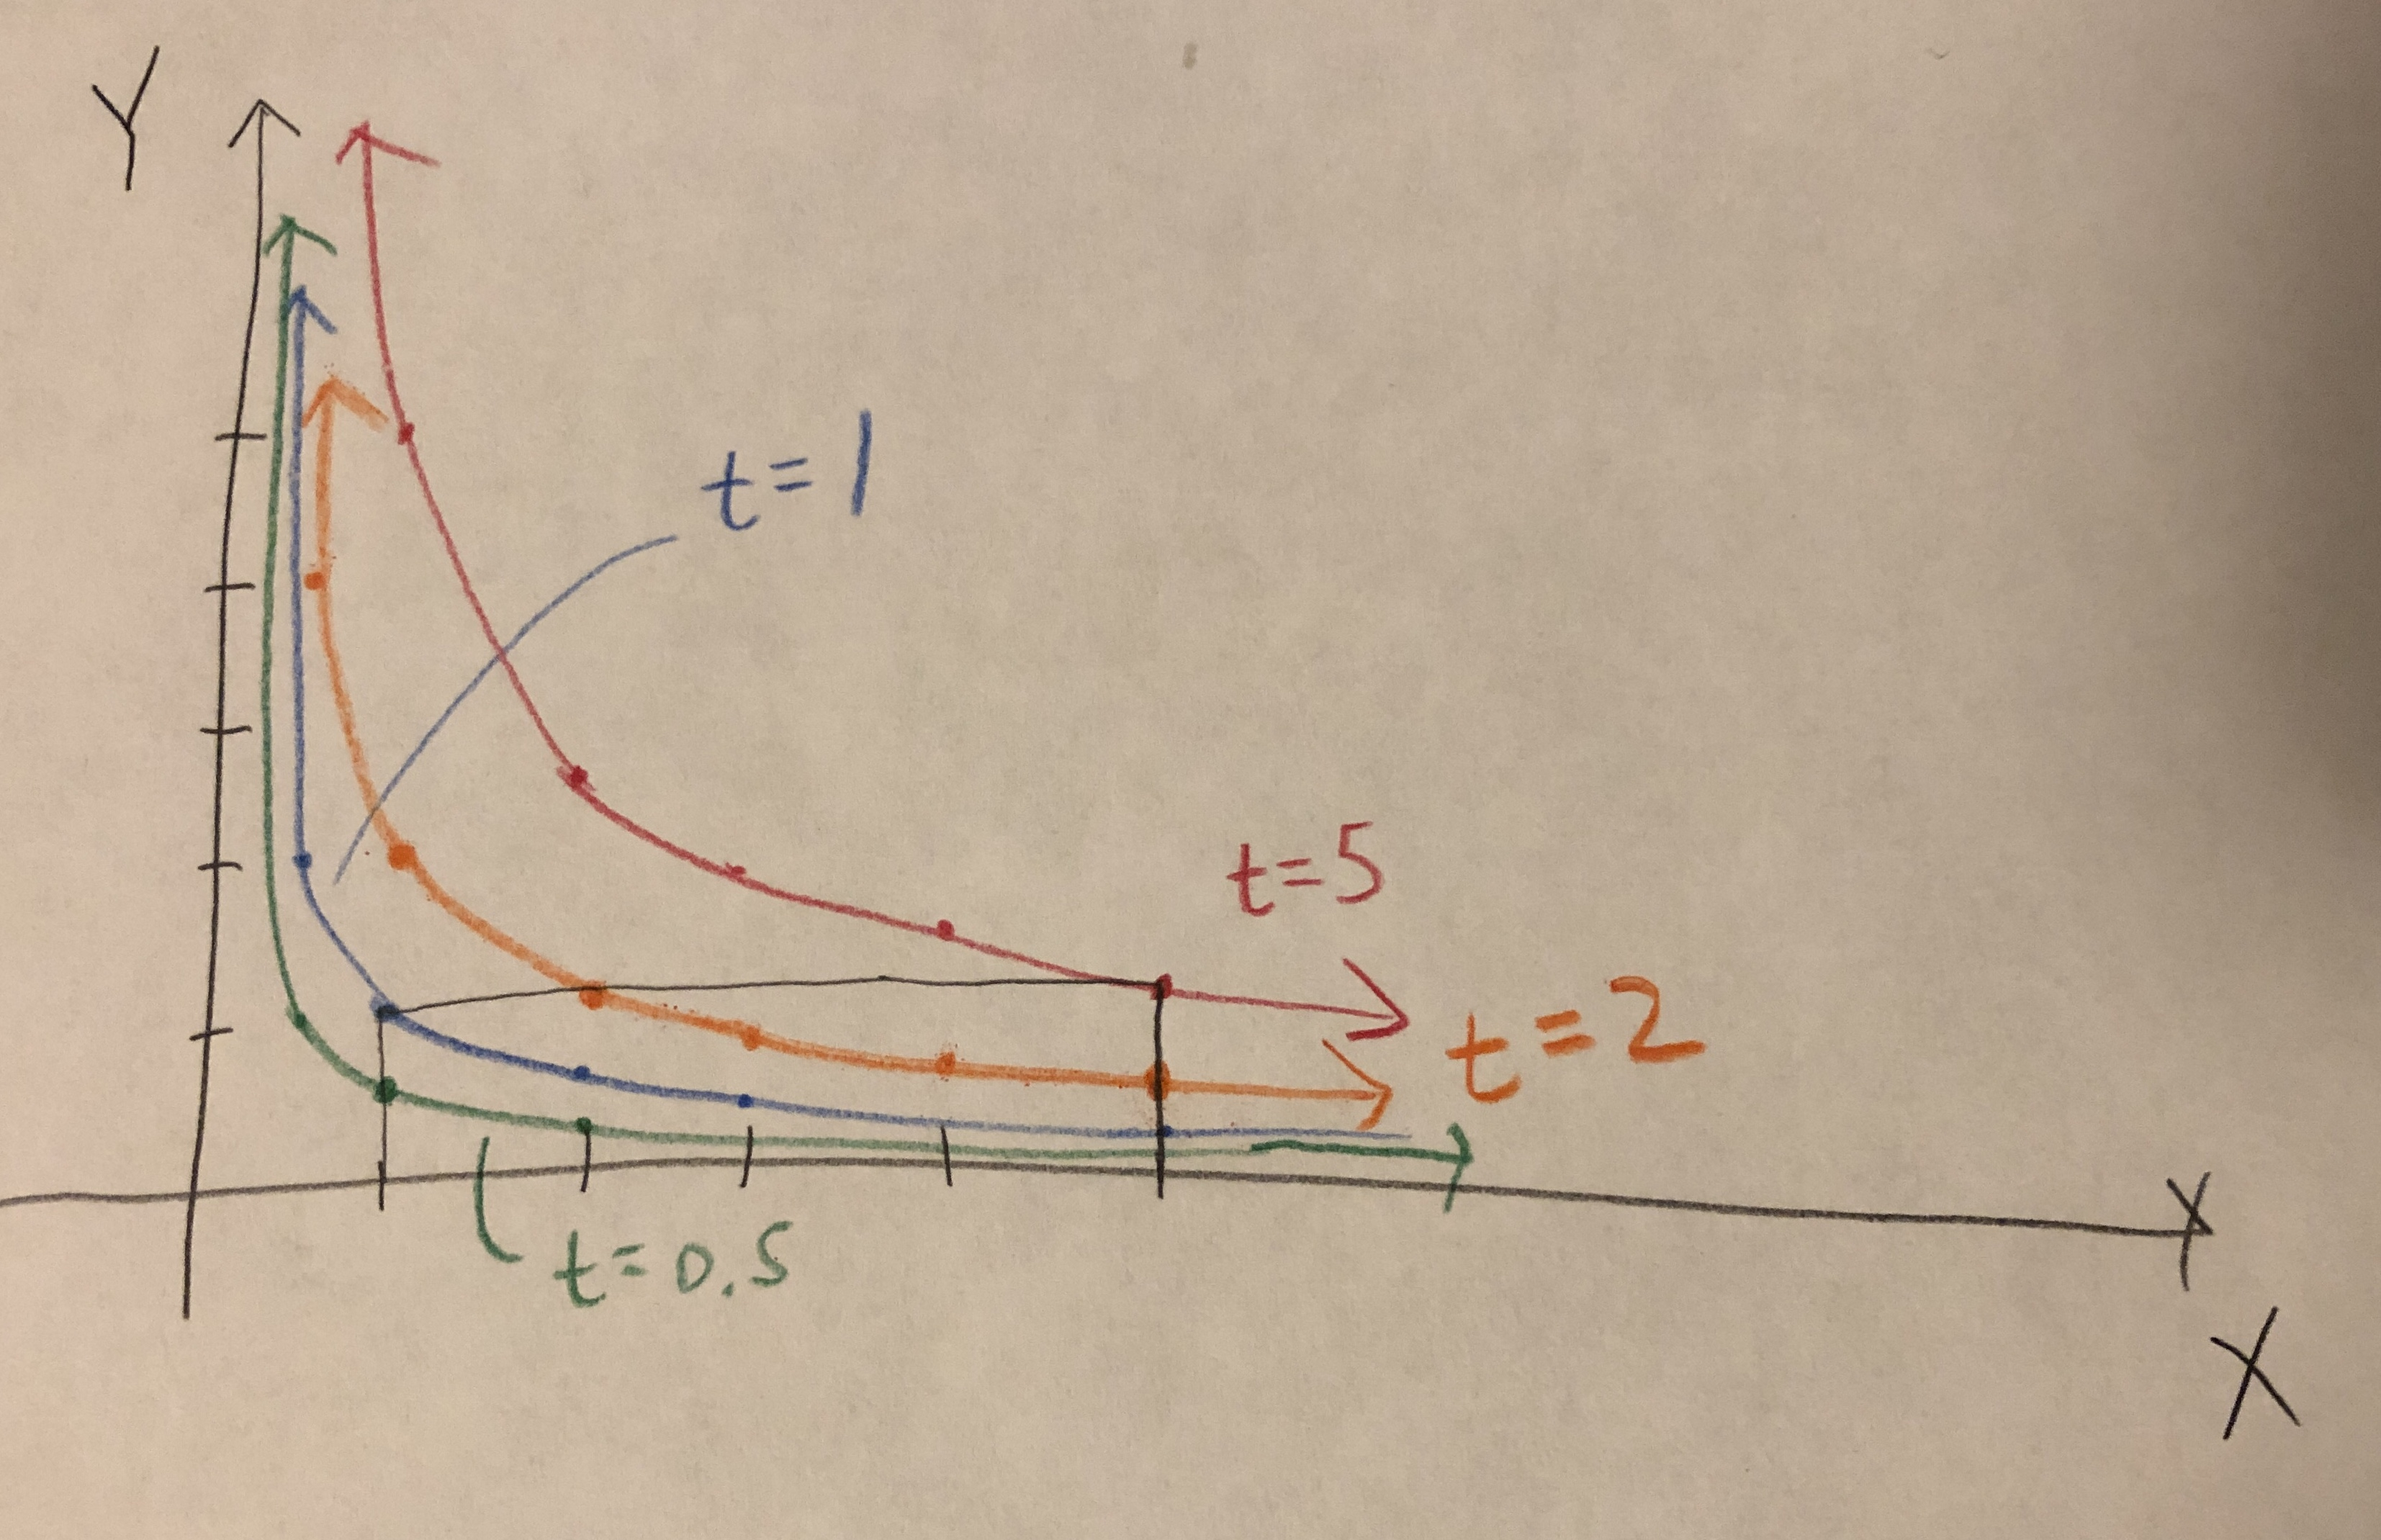
\includegraphics[width=0.8\textwidth]{prob_505a_midterm_1a}
    \end{center}
%\end{figure}

Now since both \(X\) and \(Y\) are distributed uniformly, for a given \(t\), \( \Pr(Y \leq tX^{-1})\) is the area under the curve and in the rectangle, weighted by \(1/4\) since the rectangle has total area 4 but total probability 1. It is clear that the four regimes we need to consider are (1) \(t < 0\), (2) \(0 \leq t < 1\), (3) \(1 \leq t < 5\), and (4) \(t \geq 5\). 

\begin{enumerate}[(1)]

\item \(t < 0\): The curve lies below the rectangle, so there is no area below the curve and in the rectangle. Therefore \( \boxed{\Pr(Y \leq tX^{-1} \mid t < 0) = 0}\). (This is also clear since \(tX^{-1}\) would be a negative number and \(Y\) is nonnegative.)

\item \(0 \leq t < 1\): Integrating the relevant area, we have

\[
\Pr(Y \leq tX^{-1} \mid 0 \leq t < 1) = \frac{1}{4} \int_1^5 \frac{t}{x} dx = \frac{t}{4} \big[\log(x) \big]_1^5 = \boxed{\frac{t}{4} \log(5)}
\]

\item \(1 \leq t < 5\): In this case, the area is a rectangle of height 1 and width \(t-1\) plus the area under the curve from \(t\) to 5.

\[
\Pr(Y \leq tX^{-1} \mid 1 \leq t < 5) = \frac{1}{4} \bigg( 1 \cdot (t-1) +  \int_t^5 \frac{t}{x} dx \bigg)  = \frac{1}{4} \bigg(t -1 + t\big[\log(x) \big]_t^5 \bigg) = \boxed{\frac{1}{4} \big[t \big(1+\log(5/t) \big) - 1\big]}
\]

\item \(t \geq 5\): In this case, the entire rectangle lies below the curve. Therefore \(\boxed{\Pr(Y \leq tX^{-1} \mid t \geq 5) = 1}\).

\end{enumerate}

So we have

\[
F_{XY}(t) = \begin{cases}
0 & t <0 \\
\frac{t}{4} \log(5) & 0 \leq t < 1 \\
\frac{1}{4} \big[t \big(1+\log(5/t) \big) - 1\big] & 1 \leq t < 5 \\
1 & t \geq 5
\end{cases}
\]

Finally, differentiating yields

\[
\boxed{
f_{XY}(t) = \begin{cases}
0 & t <0 \\
\frac{1}{4} \log(5) & 0 \leq t < 1 \\
\frac{1}{4} \log \bigg( \frac{5}{t} \bigg) & 1 \leq t < 5 \\
0 & t \geq 5
\end{cases}
}
\]

since

\[
\deriv{}{t} \bigg( \frac{1}{4} \big[t \big(1+\log(5/t) \big) - 1\big]  \bigg) = \frac{1}{4} \bigg[1 + \log(5/t)  + t\bigg( \frac{1}{5/t} \cdot -5 \cdot t^{-2}  \bigg) \bigg] = \frac{1}{4} \bigg[1 + \log(5/t)  + t\bigg( t\cdot -1 \cdot t^{-2}  \bigg) \bigg] 
\]

\[
= \frac{1}{4} \log \bigg( \frac{5}{t} \bigg)
\]

% 1(b)
\item \textbf{Only part included on midterm.} We will proceed in a similar way as part (a). Observe that

\[
F_{X/Y}(t) = \Pr\bigg(\frac{X}{Y} \leq t\bigg) = \Pr(Y \geq X/t)
\]

Plotting the density function of \(X/Y\) along with plots of \(F_{X/Y}(t)\) as a function of \(X\) for various values of \(t\), we have the following:


\begin{center}
    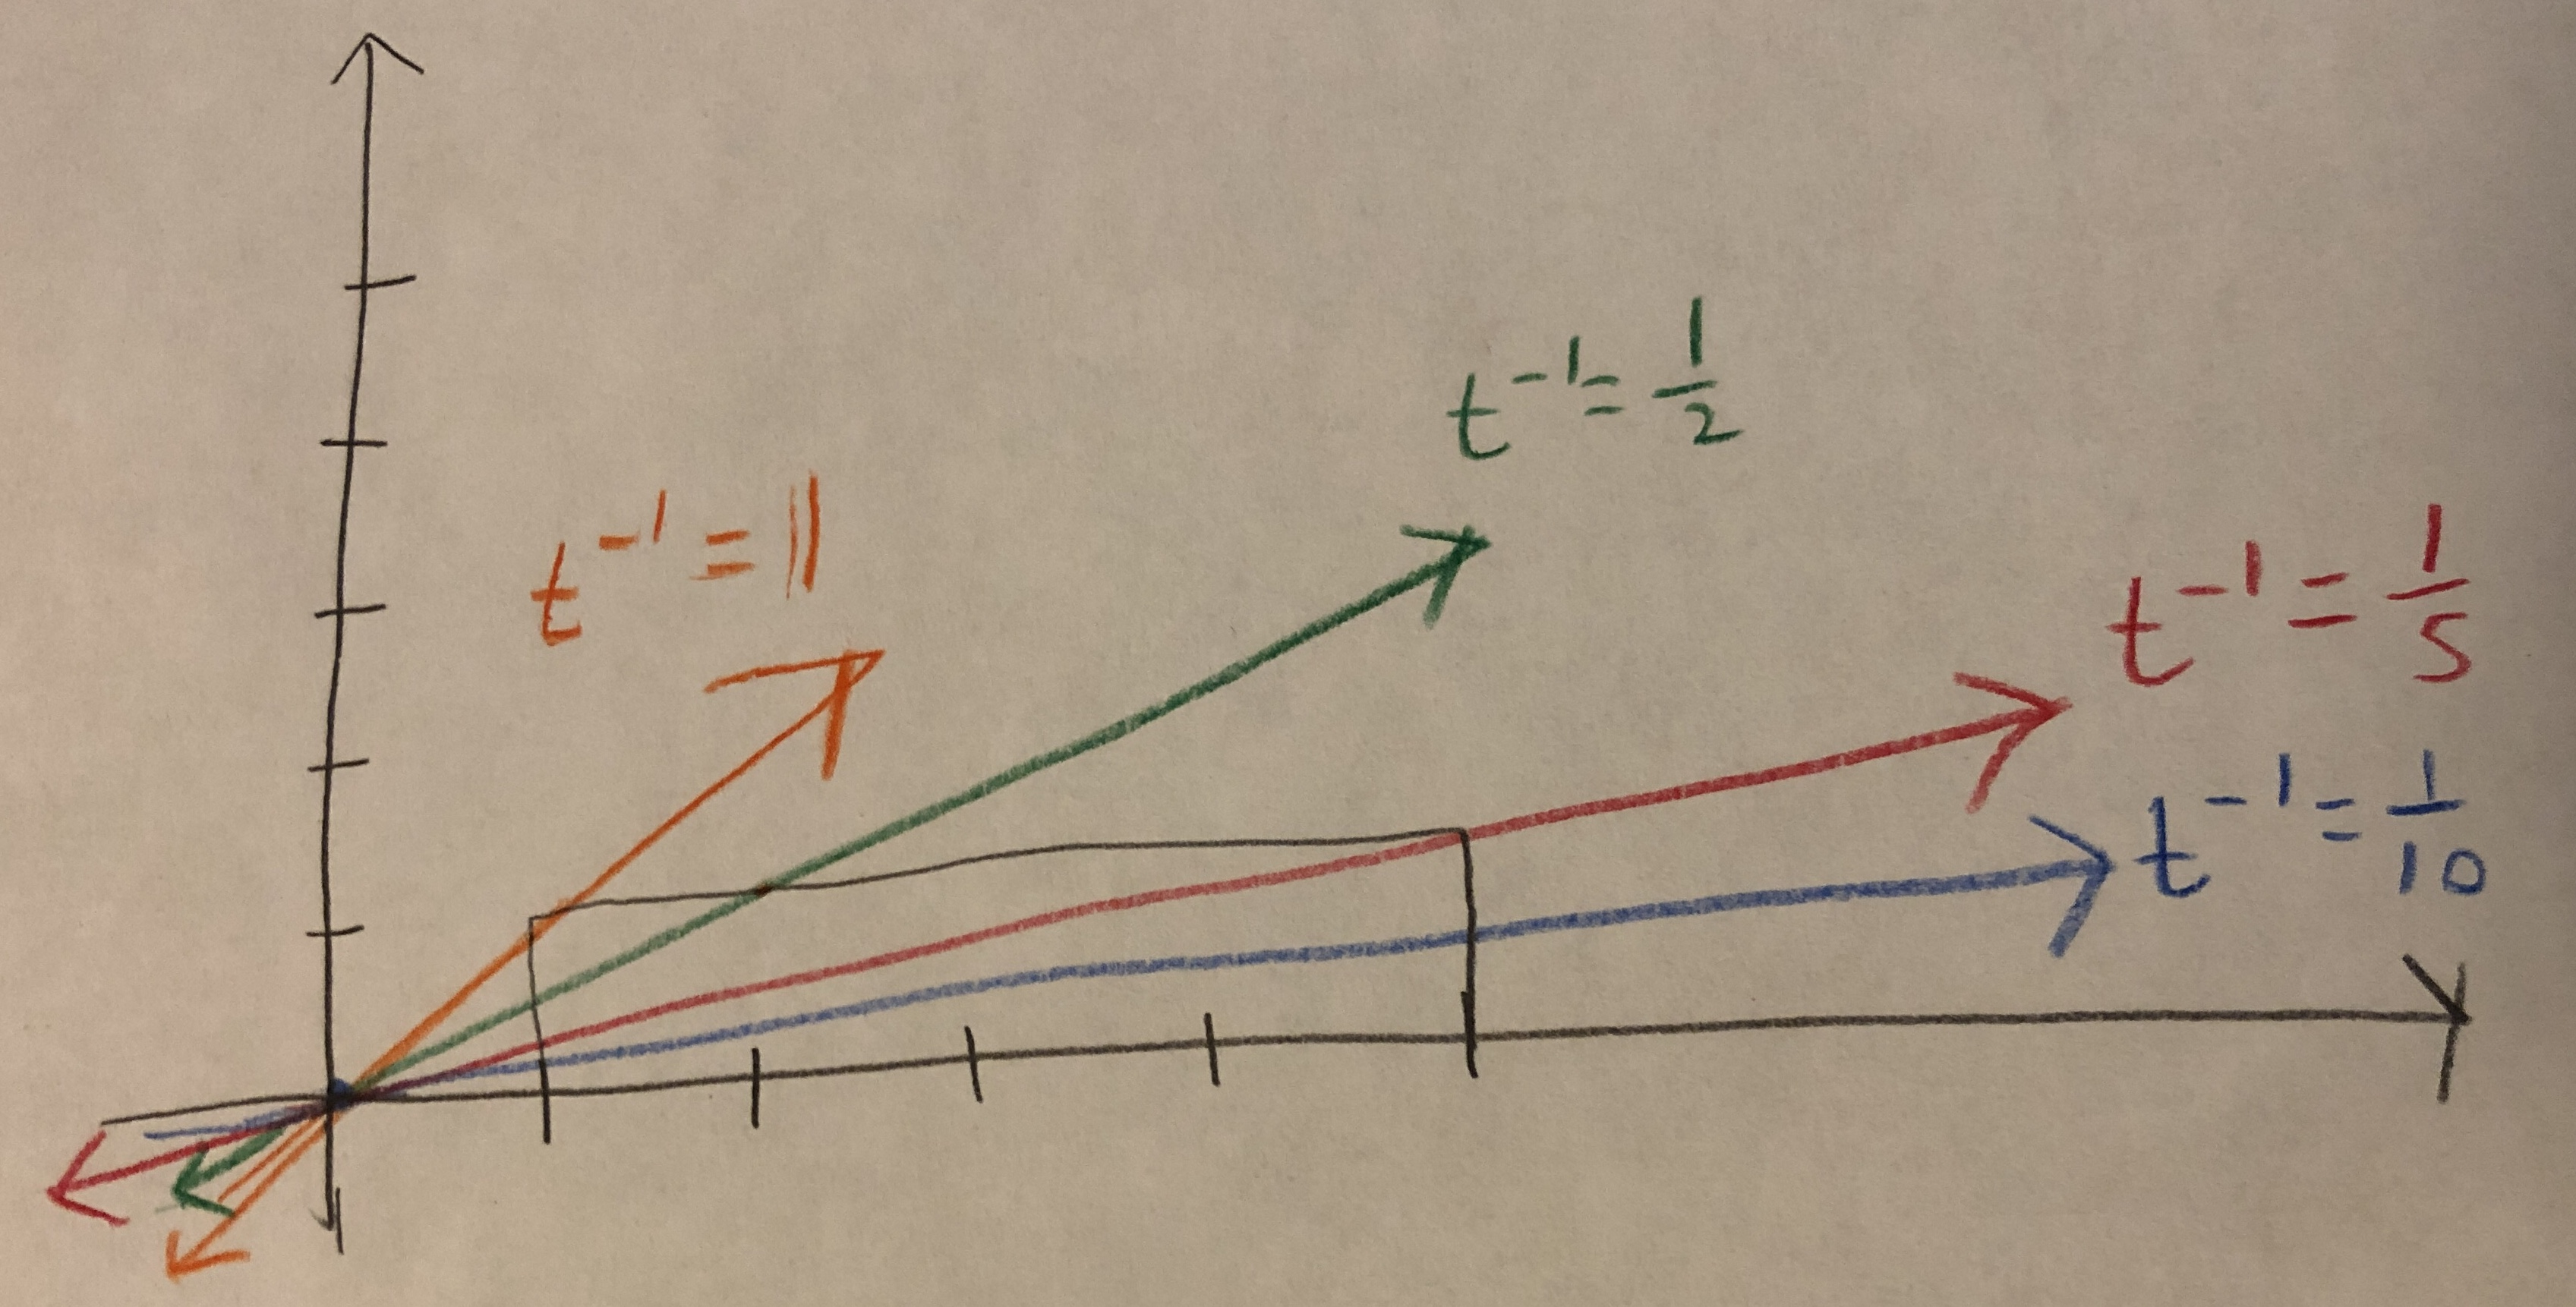
\includegraphics[width=0.8\textwidth]{prob_505a_midterm_1b}
    \end{center}


Now since both \(X\) and \(Y\) are distributed uniformly, for a given \(t\), \( \Pr(Y \geq X/t)\) is the area above the curve and in the rectangle, weighted by \(1/4\) since the rectangle has total area 4 but total probability 1. It is clear that the three regimes we need to consider are (1) \(t^{-1} \geq 1 \iff  t \leq 1\), (2) \(1/5 \leq t^{-1} < 1 \iff 1 < t \leq 5\), and (3) \(0 < t^{-1} < 1/5 \iff t > 5\). 

\begin{enumerate}[(1)]

\item \(t \leq 1\): The curve lies above the rectangle, so there is no area above the curve and in the rectangle. Therefore \( \Pr(Y \geq X/t \mid t \leq 1) = 0\). (This is also clear since \(X/t\) would have to be greater than 1 and \(Y\) is less than or equal to 1.)

\item \(1 < t \leq 5\): The relevant area is the triangle above the green line in the rectangle. Note that it intersects the vertical line at \(Y = 1/t\) and the horizontal line at \(X = t\).

\[
\Pr(Y \geq X/t \mid 1 < t \leq 5) = \frac{1}{4} \cdot \frac{1}{2}\bigg(1 - \frac{1}{t} \bigg)(t - 1) = \frac{1}{8} \bigg(t - 1 - 1 + \frac{1}{t} \bigg) = \frac{1}{8} \bigg(t -2  + \frac{1}{t} \bigg) 
\]

\item \(t > 5\): In this case, the area is a trapezoid above the blue line and in the rectangle. Note that the blue line intersects the left vertical line at \(Y = 1/t\) and the right vertical line at \(Y = 5/t\).

\[
\Pr(Y \geq X/t \mid t > 5) = \frac{1}{4} \cdot  \frac{1}{2} \cdot \bigg(1 - \frac{1}{t} + 1 - \frac{5}{t} \bigg) \cdot 4 = \frac{1}{2} \cdot \bigg(2 - \frac{6}{t} \bigg)= 1 - \frac{3}{t}
\]


\end{enumerate}

So we have

\[
\boxed{
F_{XY}(t) = \begin{cases}
0 & t \leq 1 \\
\frac{1}{8} \bigg(t -2  + \frac{1}{t} \bigg) & 1 < t \leq 5 \\
1 - \frac{3}{t} & t > 5
\end{cases}
}
\]

% 1(c)
\item The characteristic function for a uniform distribution on \([a, b]\) is 

\[
\frac{2}{(b-a)t} \sin \bigg( \frac{1}{2} (b-a)t \bigg) \exp \bigg(i(a+b) \frac{t}{2} \bigg).
\]

Using the fact that \(X \indep Y \implies \phi_{X + Y}(t) = \phi_X(t) \phi_Y(t)\), we have

\[
\phi_{X + Y}(t) = \phi_X(t) \phi_Y(t) = \frac{2}{(5-1)t} \sin \bigg( \frac{1}{2} (5-1)t \bigg) \exp \bigg(i(5+1) \frac{t}{2} \bigg)\cdot \frac{2}{t} \sin \bigg( \frac{1}{2} t \bigg) \exp \bigg(i \frac{t}{2} \bigg)
\]

\[
= \frac{1}{2t} \sin ( 2t ) \exp (3it) \cdot \frac{2}{t} \sin \bigg( \frac{1}{2} t \bigg) \exp \bigg(i \frac{t}{2} \bigg) = \boxed{ \frac{1}{t^2} \exp \bigg( \frac{7}{2}it \bigg)\cdot \sin ( 2t ) \sin \bigg( \frac{1}{2} t \bigg)}
\]

% 1(d)
\item The moment-generating function for a uniform distribution on \([a, b]\) is 

\[
M_X(t) = \E(\exp(tX)) = \int_a^b \frac{1}{b-a} \cdot \exp(tx) dx = \frac{1}{b-a} \bigg[ \frac{1}{t} \exp(tx) \bigg]_a^b =  \frac{1}{(b-a)t} \big[ \exp(bt) - \exp(at) \big]
\]

Therefore the moment-generating function for \(X\) is \(t^{-1} \big[ \exp(t) - 1\big]\). Note that
\[
\Pr(Y \leq y) = \Pr(- \log(X) \leq y) = \Pr( \log(X) \geq -y)  = \Pr(X \geq e^{-y}) = \int_{\exp(-y)}^\infty dt = \int_{\exp(-y)}^1 dt
\]

Substituting \(t = e^{-u}\) (so that we have \(u = -\log(t)\), \(dt = -e^{-u} du\), we have

\[
\Pr(Y \leq y) =  -\int_{y}^{0}  e^{-u} du = \big[e^{-u} \big]_y^0 = 1 - e^{- y}
\]
which is the cdf for an exponential distribution with mean 1. Therefore \(Y = - \log(X) \sim \operatorname{Exponential}(1)\), so

\[
M_Y(t) = \frac{1}{1- t}
\]

Using the fact that if \(X\) and \(Y\) are independent then \(M_{X +Y}(t) = M_X(t) M_Y(t)\), we have

\[
M_{X +Y}(t) = M_X(t) M_Y(t) = \frac{\exp(t) - 1}{t} \cdot \frac{1}{1- t} = \boxed{\frac{\exp(t) - 1}{t - t^2}  }
\]

\end{enumerate}


%%%%%%%%%%%%% Midterm question 5 %%%%%%%%%%%%
\item \textbf{Fall 2016 Problem 2.} Let \(X\) and \(Y\) be i.i.d. exponential with mean 1. Show that for every \(t > 0\) the events \(\{\omega: \min\{X,Y\} > t\}\) and \(\{\omega: X < Y \}\) are independent.

\textbf{Solution.} Note that \(\min\{X,Y\} > t \iff X > t \cap Y > t\). 

\begin{itemize}

\item \(\Pr(\min\{X, Y\} > t) = \Pr(X > t \cap Y > t) = \Pr(X>t) \Pr(Y > t)\)

\[
= \int_t^\infty e^{-x}dx\int_t^\infty e^{-y}dy = -e^{-x} \big|_t^\infty -e^{-y} \big|_t^\infty = \boxed{e^{-2t}}
\]

\item \(\Pr(X < Y)\): Note that in Figure \ref{prob.fig.midterm2.p5}, the region that satisfies this condition is region \(G_1\) plus \(G_2\) (note that \(X\) and \(Y\) are nonnegative). Therefore we can find this probability by integrating the joint pdf over that region.

\begin{figure}\label{prob.fig.midterm2.p5}
  \caption{Diagram for Fall 2016 Problem 2.}
  \centering
    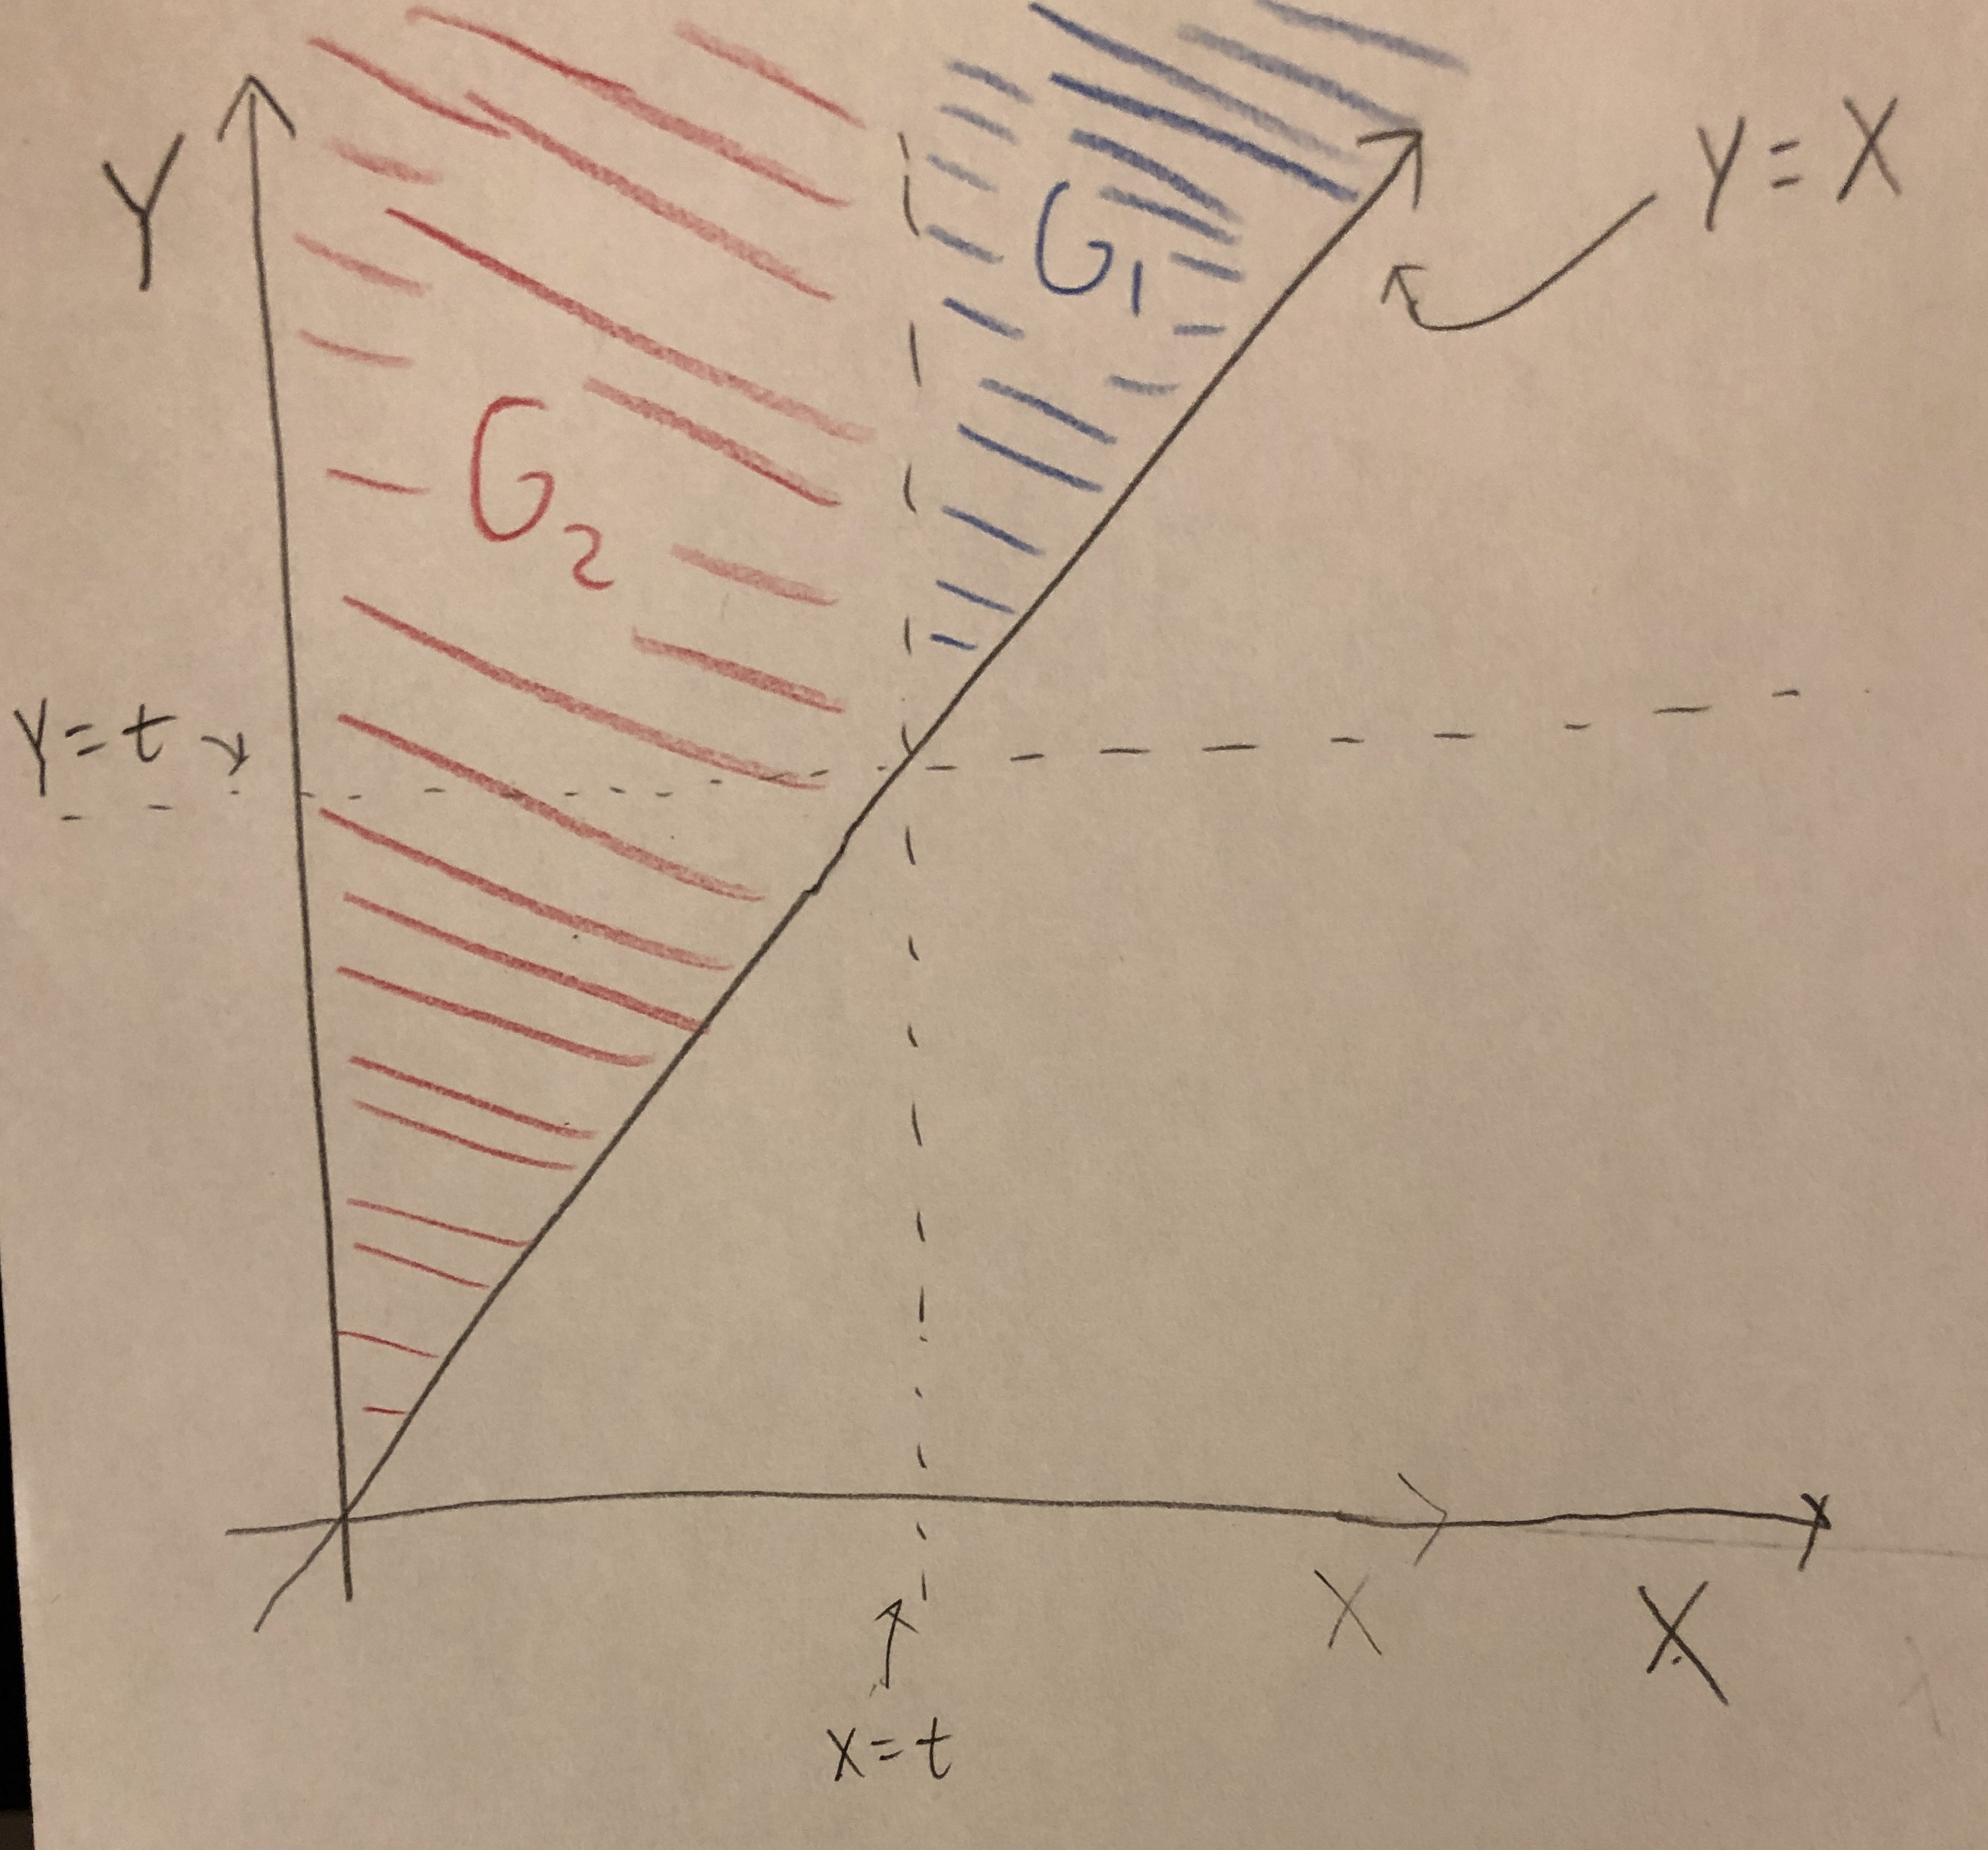
\includegraphics[width=0.7\textwidth]{prob_midterm2_p5}
\end{figure}

\[
\Pr(X < Y) = \underset{\{G_1 + G_2\}}{\int \int} f_{X,Y}(x,y) dx dy 
\]

Note that the joint pdf is the probability of the marginal pdfs since \(X\) and \(Y\) are independent.

\[
= \int_0^\infty \int_x^\infty e^{-x-y} dydx = \int_0^\infty e^{-x} \int_x^\infty e^{-y} dy dx 
\]

\[
 \int_x^\infty e^{-y} dy  = -e^{-y} \big|_x^\infty = e^{-x}
\]

\[
\implies \Pr(X < Y) = \int_0^\infty e^{-2x} dx = -\frac{1}{2} e^{-2x} \big|_0^\infty = \boxed{\frac{1}{2}}
\]



\item \(\Pr(X < Y \cap \min \{X, Y\} > t) \): Note that in Figure \ref{prob.fig.midterm2.p5}, the region that satisfies this condition is region \(G_1\). Therefore we can find this probability by integrating the joint pdf over that region.

\[
\Pr(X < Y \cap \min \{X, Y\} > t) = \underset{G_1}{\int \int} f_{X,Y}(x,y) dx dy = \int_t^\infty \int_t^y e^{-x-y} dxdy = \int_t^\infty e^{-y} \int_t^y e^{-x} dx dy
\]


\[
 \int_t^y e^{-x} dx = -e^{-x} \big|_t^y= -e^{-y} + e^{-t}
\]

\[
\implies \Pr(X < Y \cap \min \{X, Y\} > t) = \int_t^\infty e^{-y}\big(-e^{-y} + e^{-t} \big) dy =  \int_t^\infty \big( e^{-t-y} - e^{-2y}\big)dy
\]

\[
= \frac{1}{2}e^{-2y} -e^{-t}e^{-y} \big|_t^\infty = - \frac{1}{2}e^{-2t} - e^{-2t} = \boxed{\frac{1}{2}e^{-2t}}
\]

\end{itemize}

Note that

\[
\Pr(X < Y \cap \min \{X, Y\} > t)  = \frac{1}{2} \cdot e^{-2t} = \Pr(X < Y ) \Pr(\min \{X, Y\} > t)
\]

Therefore the events \(\{\omega: \min\{X,Y\} > t\}\) and \(\{\omega: X < Y \}\) are independent for every \(t > 0\).

%%%%%%%%% Final Earthquake Question %%%%%%%%%%%%%%

\item In a certain area, earthquakes happen at a frequency of one every four days. What is the probability that more than 100 earthquakes will occur in this area in one year (365 days)?

\textbf{Solution.} We can think of this as a Poisson process (see section \ref{stoch.pois.proc.sec}) with \(\lambda = 1/4\). Then there are two ways to obtain the answer: we can either examine the number of earthquakes in a 365 day period \(N(365)\) and find the probability that \(N(365) >100\), or we can examine the number of days until the 101st earthquake \(T_{101}\) and find the probability that \(T_{101} < 365\).

\begin{enumerate}[(i)]

% Poisson Approximation to earthquake problem
\item \textbf{Number of earthquakes in 365 days:} Let \(N(t)\) be the number of earthquakes that occur in \(t\) days after the start of this process. By Theorem \ref{stoch.pois.proc.thm.6.8.2}, \(N(t) \sim \operatorname{Poisson}(t \cdot 1/4)\). Then

\[
\Pr(N(t) > 100 )= \sum_{j=101}^\infty \frac{(365 \cdot 1/4)^j \exp(-365 \cdot 1/4)}{j!} 
\]

To obtain an answer for this, we can use the normal approximation to a Poisson distribution (Proposition \ref{prob.poisson.to.normal}):

\[
N(t) \sim \mathcal{N}(t/4, t/4) \implies \Pr(N(365) > 100) \approx \Pr \bigg(\mathcal{N}(0,1) > \frac{100.5 - 365/4}{\sqrt{365/4}} \bigg)
\]

\[
= \Pr \bigg(\mathcal{N}(0,1) > \frac{100.5 - 91.25}{\sqrt{91.25}} \bigg) \approx  \Pr \bigg(\mathcal{N}(0,1) > \frac{9.25}{9.1} \bigg)  \approx \boxed{0.1664}
\]

% Gamma Approximation to earthquake problem
\item \textbf{Number of days before 100th earthquake:} Let \(T_n\) be the number of days until the \(n\)th earthquake happens. By Corollary \ref{stoch.pois.proc.inter.cor}, \(T_n \sim \operatorname{Gamma}(n, 4)\). Then

\[
\Pr(T_{101} < 365 )= \int_{0}^{365} \frac{1}{\Gamma(101, 4)} x^{101 - 1} e^{-x/4} dx
\]

To obtain an answer for this, we can use the normal approximation to a Gamma distribution (Proposition \ref{prob.gamma.to.normal}):

\[
T_n \sim \mathcal{N}(404, 1616) \implies \Pr(T_{101} < 365) \approx \Pr \bigg(\mathcal{N}(0,1) < \frac{365 - 404}{\sqrt{1616}} \bigg) \approx \Pr \bigg(\mathcal{N}(0,1) < \frac{-40}{40} \bigg) 
\]

\[
=  \Pr \big(\mathcal{N}(0,1) < -1 \big)   \approx \boxed{0.1660}
\]

\end{enumerate}

\end{enumerate}
%
%
%
%
%
%
%
%
%
%
%%%%%%%%% More Problems From Homework
\subsubsection{More Problems From Homework}

%%%%%%%%%%% HW 5 P 7 %%%%%%%%%%%%%%

\textbf{Homework 5 Problem 4.}

Let \(X_1, X_2, \ldots\) be i.i.d. having moment-generating functions \(M_X = M_X(t), t \in (-\infty, \infty)\). Let \(N\) be an integer-valued random variable with moment-generating function \(M_N = M_N(t), t \in (-\infty, \infty)\). Assume that \(N\) is independent of all \(X_k\) and define \(S = \sum_{k=1}^N X_k\). Confirm that the random variable \(S\) has the moment-generating function \(M_S = M_S(t)\) defined for all \(t \in (-\infty, \infty)\) and 

\[
M_S(t) = M_N \big(M_X(t) \big)
\]

Then use the result to derive the formulae

%\[
%\E(S) = \mu_N \mu_X, \Var(S) = \sigma_N^2 \mu_X^2 + \mu_N \sigma_X^2
%\]
\[
\E(S) = \mu_N \mu_X, \Var(S) = (\sigma_N^2  -\mu_N)\mu_X^2 + \mu_N \sigma_X^2
\]

where \(\mu_N = \E(N)\), \(\mu_X = \E(X_1)\), \(\sigma_N^2 = \Var(N)\), and \(\sigma_X^2 = \Var(X_1)\). How will the above computations change if we use the characteristic function \(\phi_X\) instead of the moment-generating function \(M_X\)? 

\textbf{Solution.}

\[
M_S(t) = \E(e^{tS}) = \E[ \E(e^{tS} \mid N)] =\sum_{n=0}^\infty \E(e^{tS} \mid N = n) \Pr(N = n) =\sum_{n=0}^\infty \E(e^{t(X_1 + X_2 + \ldots + X_n)} \mid N = n) \Pr(N = n)
\]

\[
=\sum_{n=0}^\infty \E(e^{tX_1} e^{tX_2}\cdots e^{t X_n} ) \Pr(N = n)
\]

By independence of the \(X_i\) we have

\[
=\sum_{n=0}^\infty \E(e^{tX_1}) \E( e^{tX_2})\cdots \E( e^{t X_n}) \Pr(N = n)
\]

which, since the \(X_i\) are i.i.d., can be written as

\[
=\sum_{n=0}^\infty \E(e^{tX_1})^n \Pr(N = n) =\sum_{n=0}^\infty (M_X(t))^n \Pr(N = n)
\]

But since \(G_N(s) = \E(s^N) = \sum_{n=0}^\infty s^n \Pr(N = n)\), this can be written as

\[
M_S(t) = G_N(M_X(t))
\]

as desired. Note that

\[
M_S'(t) = G_N' \big( M_X(t) \big) M_X'(t)
\]

\[
M_S''(t) = G_N'' \big( M_X(t) \big) (M_X'(t))^2 + G_N' \big( M_X(t) \big) M_X''(t)
\]

So we have

\begin{itemize}

\item \(\E(S) = M_S'(0) =G_N' \big( M_X(0) \big) M_X'(0) = G_N'(1) \E(X_1) = \E(N) \E(X_1) = \mu_N \mu_X\)

\item \(\Var(S) =  \E(S^2) - \E(S)^2 = M_S''(0) - (M_S'(0))^2  \)

\[
= G_N'' \big( M_X(0) \big) (M_X'(0))^2 + G_N' \big( M_X(0) \big) M_X''(0) - \mu_N^2 \mu_X^2  = G_N'' \big( 1 \big) \E(X_1)^2 + G_N' \big( 1 \big) \Var(X_1) - \mu_N^2 \mu_X^2
\]

\[
= \E[N(N-1)] \E(X_1)^2 + \E(N) \Var(X_1) - \mu_N^2 \mu_X^2 = \E[N^2-N] \E(X_1)^2 + \E(N) \Var(X_1) - \mu_N^2 \mu_X^2
\]

\[
= [\E(N^2) - \E(N)^2 + \E(N)^2 - \E(N)] \E(X_1)^2 + \E(N) \Var(X_1) - \mu_N^2 \mu_X^2 = 
\]

\[
= [\Var(N) + \E(N)^2 - \E(N)] \E(X_1)^2 + \E(N) \Var(X_1) - \mu_N^2 \mu_X^2 = (\sigma_N^2 + \mu_N^2 -\mu_N)\mu_X^2 + \mu_N \sigma_X^2 - \mu_N^2 \mu_X^2
\]

\[
= \boxed{ (\sigma_N^2  -\mu_N)\mu_X^2 + \mu_N \sigma_X^2}
\]

\end{itemize}

To use the characteristic function \(\phi_X\) instead of the moment generating function \(M_X\), we would do the following:

\[
\phi_S(t) = \E(e^{itS}) = \E[ \E(e^{itS} \mid N)] =\sum_{n=0}^\infty \E(e^{itS} \mid N = n) \Pr(N = n) =\sum_{n=0}^\infty \E(e^{it(X_1 + X_2 + \ldots + X_n)} \mid N = n) \Pr(N = n)
\]

\[
=\sum_{n=0}^\infty \E(e^{itX_1} e^{tX_2}\cdots e^{it X_n} ) \Pr(N = n)
\]

By independence of the \(X_i\) we have

\[
=\sum_{n=0}^\infty \E(e^{itX_1}) \E( e^{itX_2})\cdots \E( e^{it X_n}) \Pr(N = n)
\]

which, since the \(X_i\) are i.i.d., can be written as

\[
=\sum_{n=0}^\infty \E(e^{itX_1})^n \Pr(N = n) =\sum_{n=0}^\infty (\phi_X(t))^n \Pr(N = n)
\]

But since \(G_N(s) = \E(s^N) = \sum_{n=0}^\infty s^n \Pr(N = n)\), this can be written as

\[
\phi_S(t) = G_N(\phi_X(t))
\]

%%%%%%%%%%% HW 5 P 7 %%%%%%%%%%%%%%

\textbf{Homework 5 Problem 7.}

\begin{enumerate}[(a)]

\item Let \(X_1, X_2, \ldots, X_n\) be independent with mean zero and finite third moment. Prove that 

\[
\E(X_1 + \ldots + X_n)^3 = \E X_1^3 + \ldots + \E X_n^3
\]

%\item Let \(X_1, \ldots, X_n\) be exponential with mean one. Prove that the random variables \(\max_{1 \leq k \leq } X_k\) and \(\sum_{k=1}^n X_k/k\) have the same distribution.

\end{enumerate}

\textbf{Solution.}

\begin{enumerate}[(a)]

% 7a
\item Let \(\E(\exp(it_iX_i) = \phi_{X_i}(t_i)\). Let \(S_n = \sum_{i=1}^n X_i\). Then by independence the characteristic function for \(S_n\) is

\[
\E(\exp(itS_n)) = \phi_{S_n}(t) = \prod_{i=1}^n \phi_{X_i}(t)
\]

Then 

\[
\E(X_1 + X_2 + \ldots + X_n)^3 = \E(S_n^3) = \phi_{S_n}^{(3)} (0)
\]

\[
= \sum_{i=1}^n \phi_{X_i}^{(3)}(0) \cdot \bigg( \prod_{j \in \{1, \ldots, n\}, j \neq i}\phi_{X_j}(0) \bigg) + C \bigg[ \sum_{i=1}^n \cdot \bigg( \sum_{j \in \{1, \ldots, n\}, j \neq i} \phi_{X_i}^{(2)} (0) \phi_{X_j}^{(1)}(0) \bigg)  \cdot \bigg( \prod_{k \in \{1, \ldots, n\}, k \neq i, j} \phi_{X_k}(0) \bigg) \bigg]
\]

where \(C\) is some coefficient resulting from the multinomial expansion of \(S_n\) after repeated differentiation product rules. But because \(\E(X_i) = 0\), \(\phi_{X_i}^{(1)} (0) = 0 \ \forall i\), so the second term goes to 0. Therefore we have

\[
\E(X_1 + X_2 + \ldots + X_n)^3  = \sum_{i=1}^n \phi_{X_i}^{(3)}(0) \cdot \bigg( \prod_{j \in \{1, \ldots, n\}, j \neq i}\phi_{X_j}(0) \bigg) = \sum_{i=1}^n \E(X_i^3) \cdot 1^{n-1} = \sum_{i=1}^n \E(X_i^3)
\]

as desired.

%% 7b
%\item 
%
%\[
%\phi_{X_i}(t) = \frac{\lambda}{\lambda - it} = \frac{1}{1 - it}
%\]
%
%An exponential distribution is itself a gamma distribution with parameters \((\lambda, 1)\). Let \(Y = \max_k \{X_k\}\). Then by independence,
%
%\[
%\Pr(Y \leq y) = \Pr(X_1 \leq y \cap X_2 \leq y \cap \cdots \cap X_n \leq y) = \Pr(X_1 \leq y) \cdot \Pr(X_2 \leq y) \cdot \ldots \cdot \Pr(X_n \leq y)
%\]
%
%Using independence, we have
%
%\[
%\phi_{Y}(t) = \prod_{i=1}^k  \frac{1}{1 - it}
%\]
%
%Let \(Z = \sum_{k=1}^n X_k/k\). By independence,
%
%\[
%\phi_{Z}(t) = \prod_{k=1}^n (\phi_{X_i}(t/k)) = \prod_{k=1}^n \frac{1}{1 - it/k}
%\]

%which is the characteristic function for a gamma distribution with parameters \((1, n)\). 


%\[
%\phi_{S_n}(t) = (\phi_{X_i}(t))^n = \bigg(  \frac{1}{1 - it} \bigg)^n
%\]
%Since the product of independent gamma distributions is gamma (Proposition \ref{prob.gammasum}), \(Y \sim \operatorname{Gamma}(1, n)\). 

%Therefore \(Y\) and \(S_n\) have the same distribution.

\end{enumerate}


%%%%%%%%%%% HW 6 P 10 %%%%%%%%%%%%%%

\textbf{Homework 6 Problem 10.}

\begin{enumerate}[(a)]

\item For \(p \in (0, 1)\), let \(x(p)\) be the smallest number of people so that there is a better than \(100 \cdot p \%\) chance to have at least two born on the same day. Find an approximate expression for \(x(p)\), and sketch the graph of the function \(x = x(p)\).

\item Repeat part (a) when you want at least three people to share a birthday.

\end{enumerate}

\textbf{Solution.} 

\begin{enumerate}[(a)]

% 10a
\item Let \(f(x)\) be the probability of no matches in birthdays in a group of \(x\) people; that is, 

\[
f(x) = \frac{365 \cdot 364 \cdot 363 \cdots (365 - x + 1)}{365^x} = \frac{1}{365^x} \cdot \frac{365!}{(365 - x)!} = \bigg( 1 - \frac{1}{365} \bigg) \bigg(1 - \frac{2}{365} \bigg) \cdots \bigg( 1 - \frac{x-1}{365}\bigg) 
\]

Using the first order Taylor approximation \(\exp(-k/x) \approx 1 - k/x\), we have

\[
f(x) = \bigg( 1 - \frac{1}{365} \bigg) \bigg(1 - \frac{2}{365} \bigg) \cdots \bigg( 1 - \frac{x-1}{365}\bigg)  \approx \exp(-1/365) \exp(-2/365) \cdots \exp(-(x-1)/365) 
\]

\[
= e^{-(x^2 - x)/(2\cdot 365)}
\]

We want the probability of a match to be at least \(p\); that is, \(f(x) \leq 1 - p\). Setting this equal to \(q = 1 - p\), we have

\[
e^{-(x^2 - x)/(2\cdot 365)} = q \iff -\frac{x^2 - x}{730} = \log(q) \iff x^2 - x + 730 \log(q) = 0 
\]

\[
\implies x = 0.5 + \sqrt{1/4 + 730 \log(1/q)} \approx \boxed{ \sqrt{2 \cdot 365 \log(1/q)}}
\]

where we discard the negative root because we have to have a nonnegative number of people, and we don't worry about the decimals since this is an approximation and we have to round up to the nearest whole person anyway.

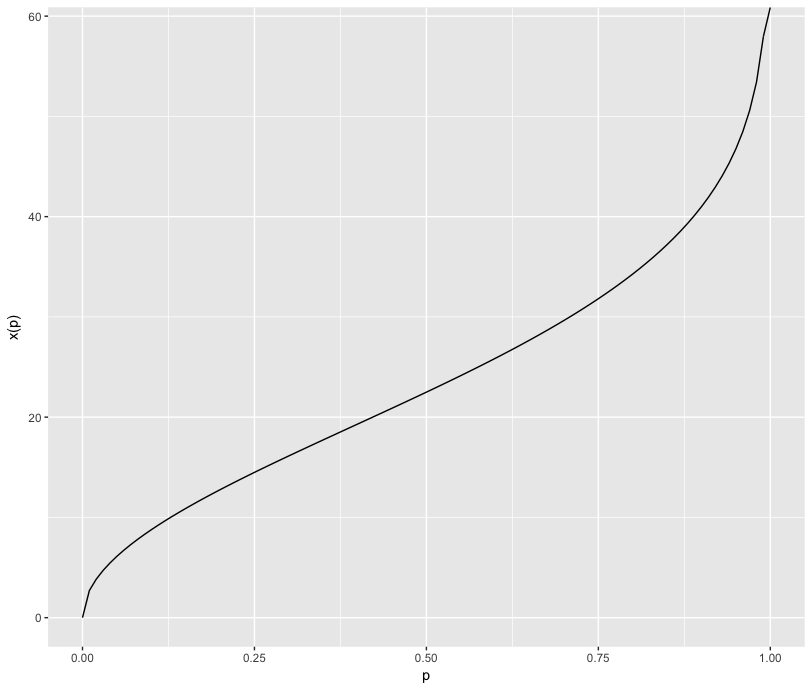
\includegraphics[scale=0.4]{prob_hw6p10a}

%We want the probability of a match to be at least \(p\); that is, \(f(x) \leq 1 - p\). Using Stirling's Formula, we have
%
%\[
%f(x) \approx  \frac{1}{365^x} \cdot \frac{365^{365} \exp(-365) \sqrt{2 \pi \cdot 365} }{(365-x)^{365-x} \exp(x-365) \sqrt{2 \pi \cdot (365-x)} } =\frac{365^{365-x} \exp(-x) \sqrt{365} }{(365-x)^{365-x} \sqrt{ 365-x }}
%\]
%
%\[
%=\frac{365^{365.5-x} \exp(-x) }{(365-x)^{365.5-x} } = \bigg( \frac{365}{365 -x} \bigg)^{365.5 - x} \cdot e^{-x}
%\]



% 10b
\item For a group of three people, the Poisson approximation (see Section \ref{prob.poisson.paradigm}) is more convenient. The number of groups of 3 people in a room of \(x\) people is \(\binom{x}{3}\). For a group of three people, the probability that all three have the same birthday is \(1 \cdot 1/365 \cdot 1/365 = 365^{-2}\). Therefore we can think of the number of matches of three people as distributed Poisson with expectation \(\binom{x}{3} \cdot 365^{-2}\). Then we have the probability of at least one ``success" (triplet with three matched birthdays) is

\[
1 - \frac{\exp(-\lambda) \lambda^0}{0!} = 1 - \exp \bigg(-\binom{x}{3} \cdot 365^{-2} \bigg)
\]

We set this equal to \(p\) and solve:

\[
p = 1 - \exp \bigg(-\binom{x}{3} \cdot 365^{-2} \bigg) \iff -\binom{x}{3} \cdot 365^{-2}  = \log(1-p) \iff \frac{x!}{(x-3)!3!} = 365^2 \cdot \log \bigg(\frac{1}{1-p} \bigg)
\]

\[
\iff x(x-1)(x-2) = 6 \cdot 365^2 \cdot \log \bigg(\frac{1}{1-p} \bigg) \iff (x^2-x)(x-2) =  x^3 - 3x^2 + 2x = 6 \cdot 365^2 \cdot \log \bigg(\frac{1}{1-p} \bigg) 
\]

This has a unique real solution, but it is hard to find.

\end{enumerate}


%%%%%%%%%%%%% Another one 

\begin{exercise}

Let \(X, Y, Z\) be independent uniform on (0, 1). Compute the cdfs of \(XY\), \(X/Y\), and \(XY/Z\). 

\end{exercise}

\begin{solution}

% \textbf{solution online: https://stats.stackexchange.com/questions/185683/distribution-of-ratio-between-two-independent-uniform-random-variables/185709}

%https://stats.stackexchange.com/questions/185683/distribution-of-ratio-between-two-independent-uniform-random-variables/185709#185709

Using the information from part (a), and the fact that \(f_X(x) = 1\) (for \(x \in [0, 1]\)) and likewise for \(f_Y(y)\):

\begin{itemize}

% Product
\item \(XY\):

\[
F_{XY}(z) = \int_0^\infty f_X(x) \int_{-\infty}^{z/x} f_Y(y) dy dx - \int_{-\infty}^0 f_X(x) \int_{\infty}^ {z/x} f_Y(y) dy dx
\]

\[
= \int_0^1  \big[ (z/x) \boldsymbol{1}_{\{0 < z/x \leq 1\}} + \boldsymbol{1}_{\{z/x > 1\}} \big] dx = \int_0^1  \big[ (z/x) \boldsymbol{1}_{\{z \leq x\}} + \boldsymbol{1}_{\{z > x\}} \big] dx = \int_0^z dx + \int_z^1 (z/x) dx
\]

\[
=z + z \log(x) \big|_z^1 = z + z \log(1) - z \log(z) = z (1 - \log(z))
\]

\[
\implies \boxed{ F_{XY}(z) =  \begin{cases} 
     0   &  z \leq 0 \\
     z (1 - \log(z)) & 0 < z \leq 1 \\
   1 & z > 1\end{cases}}
\]

% quotient
\item \(X/Y\):

\[
F_{X/Y}(z) =\int_0^\infty f_Y(y) \int_{-\infty}^{zy} f_X(x) dx dy - \int_{-\infty}^0 f_Y(y) \int_{\infty}^ {zy} f_X(x) dx dy
\]

\[
= \int_0^1  \big[ zy \boldsymbol{1}_{\{0 < zy \leq 1\}} + \boldsymbol{1}_{\{zy > 1\}} \big] dy = \int_0^1  \big[ zy \boldsymbol{1}_{\{y >0 \cap y \leq 1/z\}} + \boldsymbol{1}_{\{y > 1/z\}} \big] dy = \int_0^{1/z}zy \cdot dy + \int_{1/z}^1 dy
\]

\[
=\frac{zy^2}{2} \bigg|_0^{1/z}+ (1 - 1/z) = \frac{z}{2z^2} + 1 - \frac{2}{2z} = 1 - \frac{1}{2z}
\]

\[
\implies  F_{XY}(z) =  \begin{cases} 
     0   & z \leq 0 \\
     1 - \frac{1}{2z} & 0 < 1/z \leq 1 
     \end{cases}
\]

\[
=  \boxed{ \begin{cases} 
     0   & z \leq 0 \\
     z/2   & 0 < z \leq 1 \\
     1 - \frac{1}{2z} & z > 1
     \end{cases}}
\]

% Third thing
\item \(XY/Z\): Consider this the cdf of the quotient of \(W = XY\) and \(Z\).

\[
F_U(u)=\int_0^\infty f_Z(z) \int_{-\infty}^{uz} f_W(w) dw dz - \int_{-\infty}^0 f_Z(z) \int_{\infty}^ {uz} f_W(w) dw dz
\]

\[
=\int_0^1  \int_{0}^{uz} - \log(w)  \boldsymbol{1}_{\{0 < uz \leq 1\}} dw dz  =\int_0^1   - \big[ w \log(w) - w \big]_0^{uz} \boldsymbol{1}_{\{0 < z \leq 1/u\}}  dz  
\]

\[
=\int_0^{1/u} uz  \big[1  - \log(uz)  \big] dz = \frac{u}{4}z^2\big( 3 - 2 \log(uz) \big) \bigg|_0^{1/u}  = \frac{u}{4u^2}\big( 3 - 2 \log(1) \big) - 0 = \frac{3}{4u}
\]

\[
\implies \boxed{ F_{XY/Z}(u) =  \begin{cases} 
     0   & u \leq 0 \\
     \frac{3}{4u} & 0 < u \leq 3/4 \\
     1 & u > 3/4
     \end{cases}}
\]

\end{itemize}

\end{solution}


%
%
%
%
%
%
%
%

%\end{document}



